	
\documentclass[12pt,envcountsame,envcountchap]{svmono}
	
\usepackage[utf8]{inputenc}
\usepackage[T1]{fontenc} % high quality pdf
\usepackage{ucs} % unicode for mac os x
\usepackage{geometry} % Flexible and complete interface to document dimensions.
\geometry{a4paper}
\usepackage{graphics}
\usepackage{caption}
\usepackage{amsmath}
\usepackage{amsfonts}
\usepackage{epstopdf} % eps to pdf
\usepackage{rotating} % rotate stuff
\usepackage{lmodern} %Type1-font for non-english texts and characters
\usepackage{graphicx}        % standard LaTeX graphics tool when including figure files
\usepackage{multicol}        % used for the two-column index
\usepackage[bottom]{footmisc}% places footnotes at page bottom, etc.
\usepackage{url}
\linespread{1.2}
\usepackage{color}
\usepackage{array}
\usepackage[toc,page]{appendix}
\usepackage[acronym]{glossaries}
\usepackage{glossaries}
\usepackage{listings}
\usepackage{longtable}
\usepackage{subcaption}
\usepackage{etoolbox}% http://ctan.org/pkg/etoolbox
\usepackage{algorithm}
\usepackage{algorithmic}

\usepackage[rgb]{xcolor}
\definecolor{Highlight}{rgb}{0.84,0.47,0.10} 
\usepackage{chronology}
\usepackage{pgfgantt}

\captionsetup{compatibility=false,figurename=Figure}

\interfootnotelinepenalty=10000
%%%%%%%%%%%%%%%%%%%%%%%%%%%%%%%%%%%%%%%%%%%%%%%%%%%%%%%%

%% Use of Times New Roman font
\usefont{T1}{ptm}{m}{n}
\selectfont

\loadglsentries{001-acronyms} 	% Load list of acronyms
\makeglossaries
\glsaddall

\DeclareMathOperator*{\argmax}{arg\,max}

\renewcommand*{\glspostdescription}{}				% remove the "." at the end of the glossary description
\renewcommand{\lstlistlistingname}{List of Code Listings}		% changes the "Listing" title to "Code Listings"
\renewcommand{\lstlistingname}{Code Listing}			% changes "Listing X.Y" to "Code Listing X.Y." in text

\newcommand{\specialcell}[2][c]{						% Cell that allows break line 
  \begin{tabular}[#1]{@{}l@{}}#2\end{tabular}}
  
  
%%%% Specify table width with Left, Right or Center content of the table cell
\newcolumntype{L}[1]{>{\raggedright\let\newline\\\arraybackslash\hspace{0pt}}m{#1}}
\newcolumntype{C}[1]{>{\centering\let\newline\\\arraybackslash\hspace{0pt}}m{#1}}
\newcolumntype{R}[1]{>{\raggedleft\let\newline\\\arraybackslash\hspace{0pt}}m{#1}}

%%% Tab command
\newcommand{\tab}[1]{\hspace{.2\textwidth}\rlap{#1}}


%%% Formating listign for algorithmic entries
\renewcommand{\algorithmicrequire}{\textbf{Input:}}
\renewcommand{\algorithmicensure}{\textbf{Output:}}
\usepackage{bera}% optional: just to have a nice mono-spaced font
\usepackage{listings}
\usepackage{xcolor}

\colorlet{punct}{red!60!black}
\definecolor{background}{HTML}{EEEEEE}
\definecolor{delim}{RGB}{20,105,176}
\colorlet{numb}{magenta!60!black}

\lstdefinelanguage{json}{
    basicstyle=\normalfont\ttfamily,
    numbers=left,
    numberstyle=\scriptsize,
    stepnumber=1,
    numbersep=8pt,
    showstringspaces=false,
    breaklines=true,
    frame=lines,
    backgroundcolor=\color{background},
    literate=
     *{0}{{{\color{numb}0}}}{1}
      {1}{{{\color{numb}1}}}{1}
      {2}{{{\color{numb}2}}}{1}
      {3}{{{\color{numb}3}}}{1}
      {4}{{{\color{numb}4}}}{1}
      {5}{{{\color{numb}5}}}{1}
      {6}{{{\color{numb}6}}}{1}
      {7}{{{\color{numb}7}}}{1}
      {8}{{{\color{numb}8}}}{1}
      {9}{{{\color{numb}9}}}{1}
      {:}{{{\color{punct}{:}}}}{1}
      {,}{{{\color{punct}{,}}}}{1}
      {\{}{{{\color{delim}{\{}}}}{1}
      {\}}{{{\color{delim}{\}}}}}{1}
      {[}{{{\color{delim}{[}}}}{1}
      {]}{{{\color{delim}{]}}}}{1},
}


\begin{document}
\frontmatter 				%%%%%%%%%%%%%%%%%%%%%%%%%%%%%%%%%%%%%%%%%%%%%%%%%%%
\pagenumbering{roman}  
\begin{titlepage}
	\thispagestyle{empty}
	\begin{center}
		
\includegraphics[width=0.3\textwidth,natwidth=720,natheight=434]{./images/isellogo.png} \\[0.5cm]
		{\Large \textbf{INSTITUTO SUPERIOR DE ENGENHARIA DE LISBOA}} \\[0.5cm]
		{\Large \textbf{Área Departamental de Engenharia de \\Eletrónica e Telecomunica\c cões e de Computadores}} \\[0.8cm]		
		
\includegraphics[width=0.2\textwidth,natwidth=300,natheight=300]{./images/timetable.jpg} \\[0.8cm]
		\fontsize{18pt}{10pt}\selectfont
		{\textbf{Examination Timetabling Automation using Hybrid Meta-heuristics}} \\[0.8cm]
		\fontsize{16pt}{10pt}\selectfont
		%%%%%%%%%%%%%%%%%%%%%
		Miguel de Brito e Nunes\\[0.2cm]
		\fontsize{14pt}{10pt}\selectfont
		(Licenciado em Engenharia Informática e de Computadores)\\[0.8cm]
		\fontsize{12pt}{10pt}\selectfont
		%%%%%%%%%%%%%%%%%%%%%
		{Trabalho de projeto realizado para obten\c cão do grau\\de Mestre em Engenharia Informática e de Computadores} \\[0.8cm]
		\fontsize{16pt}{10pt}\selectfont
		Relatório Provisório
		\vfill
		\begin{tabbing}
		   \fontsize{12pt}{10pt}\selectfont
		   Orientadores: \\
		   \fontsize{11pt}{10pt}\selectfont
		   \hspace{1.1cm}Doutor Artur Jorge Ferreira \\
		   \fontsize{11pt}{10pt}\selectfont
		   \hspace{1.1cm}Mestre Nuno Miguel da Costa de Sousa Leite \\
		\end{tabbing}
		%\begin{tabbing}
		   %\fontsize{12pt}{10pt}\selectfont
		   %Júri: \\
		   %\fontsize{11pt}{10pt}\selectfont
		   %\hspace{1.1cm}Presidente: Mestre Fernando Manuel Gomes de Sousa \\
		   %\fontsize{11pt}{10pt}\selectfont
		   %\hspace{1.1cm}Vogais: \\
		   %\fontsize{11pt}{10pt}\selectfont
		   %\hspace{2.2cm}Mestre Artur Jorge Ferreira \\
		   %\fontsize{11pt}{10pt}\selectfont
		   %\hspace{2.2cm}Doutor Luís Filipe Graça Morgado\\
		   %\fontsize{11pt}{10pt}\selectfont
		   %\hspace{2.2cm}Mestre Luís Manuel da Costa Assunção\\
		%\end{tabbing}
		
		\fontsize{10pt}{10pt}\selectfont
		\textbf{Setembro, 2015}
	\end{center}

	\newpage
	\thispagestyle{empty}
	\cleardoublepage
	\newpage
	\thispagestyle{empty}
	
	\begin{center}
		
\includegraphics[width=0.3\textwidth,natwidth=720,natheight=434]{./images/isellogo.png} \\[0.5cm]
		{\Large \textbf{INSTITUTO SUPERIOR DE ENGENHARIA DE LISBOA}} \\[0.5cm]
		{\Large \textbf{Área Departamental de Engenharia de \\Eletrónica e Telecomunica\c cões e de Computadores}} \\[0.8cm]		
		
\includegraphics[width=0.2\textwidth,natwidth=300,natheight=300]{./images/timetable.jpg} \\[0.8cm]
		\fontsize{18pt}{10pt}\selectfont
		{\textbf{Examination Timetabling Automation using Hybrid Meta-heuristics}} \\[0.8cm]
		\fontsize{16pt}{10pt}\selectfont
		%%%%%%%%%%%%%%%%%%%%%
		Miguel de Brito e Nunes\\[0.2cm]
		\fontsize{14pt}{10pt}\selectfont
		(Licenciado em Engenharia Informática e de Computadores)\\[0.8cm]
		\fontsize{12pt}{10pt}\selectfont
		%%%%%%%%%%%%%%%%%%%%%
		{Trabalho de projeto realizado para obten\c cão do grau\\de Mestre em Engenharia Informática e de Computadores} \\[0.8cm]
		\fontsize{16pt}{10pt}\selectfont
		Relatório Provisório
		\vfill
		\begin{tabbing}
		   \fontsize{12pt}{10pt}\selectfont
		   Orientadores: \\
		   \fontsize{11pt}{10pt}\selectfont
		   \hspace{1.1cm}Doutor Artur Jorge Ferreira \\
		   \fontsize{11pt}{10pt}\selectfont
		   \hspace{1.1cm}Mestre Nuno Miguel da Costa de Sousa Leite \\
		\end{tabbing}
		%\begin{tabbing}
		   %\fontsize{12pt}{10pt}\selectfont
		   %Júri: \\
		   %\fontsize{11pt}{10pt}\selectfont
		   %\hspace{1.1cm}Presidente: Mestre Fernando Manuel Gomes de Sousa \\
		   %\fontsize{11pt}{10pt}\selectfont
		   %\hspace{1.1cm}Vogais: \\
		   %\fontsize{11pt}{10pt}\selectfont
		   %\hspace{2.2cm}Mestre Artur Jorge Ferreira \\
		   %\fontsize{11pt}{10pt}\selectfont
		   %\hspace{2.2cm}Doutor Luís Filipe Graça Morgado\\
		   %\fontsize{11pt}{10pt}\selectfont
		   %\hspace{2.2cm}Mestre Luís Manuel da Costa Assunção\\
		%\end{tabbing}
		
		\fontsize{10pt}{10pt}\selectfont
		\textbf{Setembro, 2015}
	\end{center}


	
\end{titlepage}


%\chapter*{Acknowledgments}
\addcontentsline{toc}{chapter}{Acknowledgments} 
I would like to express my gratitude to my supervisors Artur Ferreira and Nuno Leite, whose understanding, advices and orientation considerably increased my knowledge and overall quality of the developed project. I sincerely appreciate their assistance during the writing of the document in cause.\\
\\
I would also like to thank my mother and father, Tetyana and Valery, for supporting my decisions during my entire life, which have helped to become the person I am. A heartfelt thanks goes out to my girlfriend Carina, for all your love, support and motivation that you have given.\\
\\
Last, but not least, I would like to thank the Instituto Superior de Engenharia de Lisboa, which have been one of my main occupations for the past 5 years, and had prepared me for the IT Engineering world.

\chapter*{Resumo}
\addcontentsline{toc}{chapter}{Resumo} 
Nos últimos anos, com a proliferação de dispositivos móveis, tais como \textit{smartphones}, as pessoas estão em constante troca de informação. Por exemplo, no contexto de visitas turísticas, as pessoas têm sempre o \textit{smartphone} presente, o que lhes possibilita a consulta da informação sobre o ponto turístico escolhido. Quando se visita um determinado local, a aplicação de guia turístico recomenda informações úteis para o utilizador. Estas recomendações são baseadas na localização atual do utilizador, nas suas preferências e visitas anteriores, possibilitando ainda que seja fornecida a opinião do mesmo sobre cada visita.\\
\\
Neste relatório, abordamos o desenvolvimento da aplicação móvel e a correspondente aplicação \textit{Web}, denominada GuideMe, para consulta, divulgação e recomendação de locais turísticos. A aplicação móvel foi desenvolvida para a plataforma iOS, seguindo o conceito de \textit{Universal Application}, suportando os dispositivos iPhone, iPad e iPod Touch. O serviço na sua totalidade, oferece um conjunto de funcionalidades que melhoram a experiência do utilizador durante as visitas dos locais turísticos. O foco principal da aplicação móvel, é o de apresentar os locais turísticos na vizinhança da posição atual do utilizador. A informação sobre a localização atual é representada sob a forma de coordenadas geográficas (latitude e longitude), obtidos pelo dispositivo móvel através do equipamento Global Positioning System (GPS) ou através da triangulação de antenas WiFi. Os utilizadores também têm acesso a opções de filtragem únicas aquando da pesquisa dos locais turísticos. A pesquisa pode-se basear na sua disponibilidade para a visita, condições meteorológicas do local e altura preferida do dia (dia ou noite). Cada utilizador pode consultar os pontos turísticos, marca-los como visitados ou por visitar. Posteriormente, o sistema irá usar esta informação para calcular as recomendações dos locais que não foram previamente visitados pelo utilizador.\\
\\
A infra-estrutura que suporta o serviço GuideMe implementa o próprio sistema de recomendação, que tem como objetivo analisar as visitas de cada utilizador e construir listas de recomendação baseando-se nos gostos mútuos entre os utilizadores. As recomendações produzidas são adequadas ao gosto do utilizador em causa. Com o sucesso do sistema de recomendação da Amazon, este tema tem sido o alvo do estudo e contribuição constante nos últimos anos. Através da literatura analisada, teve-se a oportunidade de estudar as diversas metodologias e algoritmos que compõem os sistemas de recomendação atuais. Analisamos as vantagens e desvantagens das seguintes abordagens e metodologias: Filtragem Baseada em Conteúdo (FBC); Filtragem Colaborativa baseada em Itens (FCBI); Filtragem Colaborativa baseada em Utilizadores (FCBU); Sistemas Híbridos. A literatura justifica que os sistemas mais robustos e de maior qualidade são baseados em abordagens híbridas. Na sua vertente simples, um sistema híbrido é composto pela junção do FBC com FCBI ou FCBU, que minimiza os pontos fracos de cada um dos sistemas.\\
\\
Apesar da eficiência e da qualidade dos sistemas híbridos, devido à sua elevada complexidade de implementação, a abordagem escolhida para este projeto é a FCBI. Realizamos o estudo e a avaliação estatística dos diversos fatores (desempenho, tempo de execução e a dimensão de dados) que nos possibilitaram concluir que o algoritmo Slope One é o mais adequado para o sistema de recomendação em questão. A computação das recomendações é realizada periodicamente, agendada pelo \textit{Cron job} para as 3:00 da manhã, em cada dia. O serviço seleciona um conjunto de utilizadores com as novas visitas e atualiza a sua lista de recomendações.\\
\\
O serviço GuideMe foi implementado com uma arquitetura de 3 camadas, composta pela camada de dados, camada lógica de negócio e camada de apresentação. A primeira é responsável por armazenar a informação num modelo relacional MySQL. Qualquer operação sobre o modelo de dados é realizada através da camada de acesso a dados, implementada com recurso à \textit{framework} Hibernate. Na camada de negócio posiciona-se a componente de sistema de recomendação e a RESTful API. A API expõe um conjunto de \textit{endpoints} a serem consumidos pelas aplicações clientes, é responsável pela sua segurança, autenticação, formato de dados, entre outros. O serviço de recomendação encontra-se implementado sob a forma de uma biblioteca, enquanto que a API RESTful é implementada com recurso à \textit{Play Framework} como uma aplicação \textit{Web}. Ambas as componentes acedem aos dados usando a mesma camada de acesso a dados.\\
\\
A estabilidade do serviço foi avaliada através de testes de carga. Estes ajudaram a detectar os pontos fracos do sistema, implicando melhorias a nível de estabilidade e robustez do serviços desenvolvidos.\\
\\
A aplicação móvel e a aplicação Web, utilizam os mesmos \textit{endpoints} da API RESTful para consulta, publicação e edição dos dados. Suportam a autenticação através dos serviços sociais comuns para a atualidade, nomeadamente Facebook e Twitter. Ambas as aplicações suportam o conceito de internacionalização. Atualmente encontram-se em Inglês e Português, mas a infra-estrutura implementada possibilita uma fácil adição de novos idiomas. A internacionalização constituiu um desafio no desenho da arquitetura do sistema, é uma funcionalidade que teve de ser integrada desde o modelo relacional, até à camada de acesso a dados, API RESTful e as respetivas aplicações Web e móvel.\\
\\
A aplicação Web implementa um subconjunto de funcionalidades da aplicação móvel, esta foi desenvolvida com o objetivo de provar o correto funcionamento da RESTful API demonstrando que várias aplicações clientes conseguem consumir a mesma fonte de informação. Atualmente a interface do \textit{backoffice} é implementada pela aplicação móvel que pode ser apenas acedida por utilizadores com privilégios especiais. Em modo de administração é possível realizar operações tais como: editar a informação de um local; adicionar novos locais; consultar a informação reportada pelos utilizadores sobre os dados incorrectos de um local; e visualizar os erros das diferentes componentes do serviço. No futuro, pretende-se com que a aplicação Web tenha o mesmo conjunto de funcionalidades da aplicação móvel. Foi o que diz respeito ao \textit{backoffice}, de modo a facilitar a gestão do sistema em algumas situações.\\
\\
As aplicações desenvolvidas providenciam uma interface agradável e de simples utilização. Foi conduzida uma avaliação de usabilidade da aplicação móvel, que nos possibilitou identificar o público alvo, as suas preferências e a opinião que obtiveram ao utilizar a aplicação GuideMe. Na análise realizada, a avaliação geral foi positiva e a maioria das pessoas mostrou interesse em utilizar a aplicação no futuro.\\
\\
É expectável que a solução atual seja posta em prática e que contribua de forma positiva para o aumento de turismo nos locais menos conhecidos.

\section*{Palavras Chave}
GuideMe; Guia Turístico; Aplicação Móvel; Aplicação Web; Sistema de Recomendação; iOS; iPhone; iPad; REST

\chapter*{Abstract}
\addcontentsline{toc}{chapter}{Abstract} 
In the past few years, with the proliferation of mobile devices such as smartphones, people are experiencing frequent communication and information exchange. For instance, in the context of tourist visits, it is often the case that each person carries out a smartphone, to consult information about a chosen point of interest. When one visits a given location, a suitable tourist guide application will recommend useful information to the tourist, based on its current location, preferences, past visits, further allowing the user to provide feedback about each visit.\\
\\
In this report, we address the development of a mobile application and the corresponding Web application, named GuideMe, for consultation, publication, and recommendation of touristic locations. Users are offered features that improve their experience when they visit some touristic location. Each user may consult places of touristic interest, receive suggestions of previously unseen touristic places according to past users recommendations, and to perform its own recommendations. The GuideMe service offers a set of search filters, based on several criteria (such as the distance between user and point of interest location and the user’s available time, among others) to facilitate the exploration of new locations. The key novelties of GuideMe, as compared to previous approaches, lies in the use of a recommendation process and the social interaction between users.\\
\\
The evaluation of the different recommendation algorithms has contributed to the quality of the implemented recommender system. The load tests have helped to detect some weak spots and improve overall the stability and robustness of the developed service.

\section*{Keywords}
GuideMe; Tourist Guide; Mobile Application; Web Application; Recommender System; iOS; iPhone; iPad; REST


%%% The followinf 3 commands will force page number to 
%%% appear on every page after the cover pages
\makeatletter
\let\ps@empty\ps@plain
\makeatother

\pagestyle{plain} 
\setcounter{tocdepth}{3}
\tableofcontents
\listoffigures	
\addcontentsline{toc}{chapter}{List of Figures} 
\listoftables
\addcontentsline{toc}{chapter}{List of Tables}
\lstlistoflistings
\addcontentsline{toc}{chapter}{List of Code Listings}

\printglossary[type=\acronymtype, nonumberlist, title=List of Acronyms, style=listwithwidth]
\addcontentsline{toc}{chapter}{List of Acronyms}

\mainmatter 					%%%%%%%%%%%%%%%%%%%%%%%%%%%%%%%%%%%%%%%%%%%%%%%%%%
\pagenumbering{arabic}

\setcounter{secnumdepth}{3}
\chapter{Introduction}
\label{introduction}
\thispagestyle{plain}

Many people believe that AI (Artificial Intelligence) was created to imitate human behavior and the way humans think and act. Even though people are not wrong, AI was also created to solve problems that humans are unable to solve, or to solve them in a shorter amount of time, with a better solution. Humans may take days to find a solution, or may not find a solution at all that fits their needs. Search algorithms may deliver a very good solution in minutes, hours or days, depending on how much time the human is willing to use in order to get a better solution. \\
\\
%%%%%%%%%%%%%%%
A concrete example is the creation of timetables. Timetables can be used for educational purposes, sports scheduling, transportation timetabling, among other applications. The timetabling problem consists in scheduling a set of events (e.g., exams, people, trains) to a specified set of time slots, while respecting a predefined set of rules. These rules are called constraints in the timetabling subject, making harder to achieve a solution for the problem. In some cases the search space is so limited by the constraints that one is forced to "relax" them in order to find a solution. \\
\\
%%%%%%%%%%%%%%%
Solutions can be divided in multiple types, like \textit{feasible solutions}, \textit{non feasible solutions}, \textit{optimal solutions} or \textit{sub-optimal solution}. A feasible solution is a solution that solves all the mandatory problem constraints, in contrary to non feasible solutions. An optimal solution is the best feasible solution possible considering the problem and its optimal solution value. It's possible for a problem to have multiple optimal solutions. For last, non-optimal solutions are feasible solutions that can't reach the optimal solution value and so are not as good compared to an optimal solutions.\\
\\
%%%%%%%%%%%%%%%
The process of creating a timetable requires that the final solution follows a set of constraints. These can be divided in two groups: \textit{hard constraints} and \textit{soft constraints}. Hard constraints are a set of rules which must be followed in order to get a feasible solution. On the other hand, soft constraints represent the views of the different interested parties (e.g. institution, students, nurses, train operators) in the produced timetable. The satisfaction of these type of constraints is not mandatory as is the case of the hard constraints. In the timetabling problem, the goal is usually to optimize a function comprehending a weighted combination of the different soft constraints, while satisfying the set of hard constraints. \\
\\
%%%%%%%%%%%%%%%
The goal of the present project is to create an examination timetable generator using the ITC 2007 (International Timetabling Competition) specification. The solutions will be validated using a validator developed for this purpose in order to assess the quality of the solution. It is also required that the developed prototype may work with two exam epochs which can be considered an extension to the ITC-2007 formulation. In the end an (optional) Graphical User Interface will be created in order to allow the user to edit the current solution to fit the users needs and and to allow the optimization of the edited solution. The generator will be tested using data from ITC-2007 and some actual data from six different programs lectured at ISEL.
%%%%%%%%%%%%%%%
\section{Examination timetabling: State of the Art}
\label{sec:sota}
In this Section, we review the state of the art of problem at hand. We start by describing why timetabling is a rather complex problem, some possible approaches on trying to solve the problem and some of the solutions already taken, specifically for ITC 2007 data.
\\
%%%%%%%%%%%%%%%%%%%%
\subsection{Timetabling Problem}
%%%%%%%%%%%%%%%%%%%%
Timetabling is a subject that has been a target of research for about 50 years. Its problem may be formulated as a search or optimization problem [REF: 1999 Schaerf]. As a search problem, the goal consist on finding a solution (feasible solution) that satisfies all the hard constraints, while ignoring the soft constraints. On the contrary, posing the timetabling problem as an optimization problem, one wants to find the best solution possible with time constraints. That is, one seeks to minimize (considering a minimization problem) the violations of soft constraints while satisfying the hard
constraints. Typically, the optimization is done after using a search procedure for finding an initial feasible solution.
\\
%%%%%%%%%%%%%%%
The basic examination timetabling problem, where only the clash hard constraint is observed, reduces to the graph coloring problem [REF: Jensen, Tommy R.; Toft, Bjarne (1995), Graph Coloring Problems, John Wiley and Sons]. This is a well studied hard problem. Deciding whether a solution exists in the Graph Coloring problem is a NP-complete problem [ref. Arora and Barak book titled "Computational Complexity"]. Considering the graph coloring as an optimization problem, it is proven that the task of finding the optimal solution is a NP-Hard problem [ref. Arora and Barak book titled "Computational Complexity"]. Graph Coloring problems are explained further in ~\ref{subsection:graphcoloring}
\\
%%%%%%%%%%%%%%%%%%%%
\subsection{Existing approaches}
\label{subsection:ExistingAppr}
%%%%%%%%%%%%%%%%%%%%
Timetabling solution approaches are usually divided in the following categories [REF: survey R. Qu]: \textit{exact algorithms} (Branch-and-Bound, Dynamic Programming), \textit{graph based sequential techniques} (Saturation degree, Colour degree, Largest degree), \textit{local search based techniques} (Tabu Search, Simulated Annealing (SA), \textit{population based algorithms} (Evolutionary Algorithms, Memetic algorithms, Ant algorithms, Artificial immune algorithms), \textit{Multi-criteria techniques}, \textit{Hyper-heuristics}, \textit{Decomposition/clustering techniques} and \textit{hybrid algorithms}, which combine features of several algorithms, comprise the state-of-the-art. Due to its complexity, approaching the examination timetabling problem using exact method approaches can only be done for small size instances. Real problem instances found in practice are usually of large size, making the use of exact methods impracticable. Heuristic solution algorithms have usually employed to solve this problem.

Real problem instances are usually solved by using both Heuristics and Meta-heuristics algorithms. Heuristic algorithms are problem-dependent, meaning that these are adapted to a specific problem in which take advantage of its details. Heuristics are used to generate a feasible solution, focusing on solving all hard constraints only. Meta-heuristics on the other hand are problem-independent. These are used to, given the feasible solution obtained using heuristic algorithms, generate a better solution focusing on solving as many soft constraints as possible.\\
\\
Most of the Meta-heuristic algorithms used belong to one of the three categories: One-Stage algorithms, Two-Stage algorithms and Algorithms that allow relaxations. [REF: 2008 - Rhydian Lewis]. 
\begin{itemize}
  \item The One-Stage algorithm is used to get an initial optimal solution, which the goal is to satisfy both hard and soft constraints at the same time. Approaches using this stage are not very common because it's hard to get proper solutions in a reasonable amount of time trying to satisfy both types of constraints at the same time;
  \item The Two-Stage algorithms are the most used types of approaches because is is divided in two phases (the reason for "Two-Stage" name). The first phase consists in all soft constraints being "discarded" and focus only on solving hard constraints to obtain a feasible solution. The next phase is an attempt to find the best solution, trying to solve the highest number of soft constraints possible given the solution of the first phase.
\end{itemize}

\subsubsection{Exact methods}
\label{subsection:exactmethods}
Some approaches may use \textit{exact methods} which may be viewed as tree algorithms and can be proved that it can find the optimal solution (global optimal). Exact methods search for solutions in the whole search space, and they divide the global problem into simpler problems in order to find the solution. This is not always used because these methods require a lot of computing time and they rarely produce results in a reasonable time in complex problems. Some approaches use some of these exact methods, namely: Constraint Programming Based Technique, Integer Linear Programming.\\

\paragraph{Constraint Programming Based Technique}
The Constraint Programming Based Technique (CPBT) allows direct programming with constraints which gives ease and flexibility in solving problems like timetabling. Two important features about this technique are backtracking and logical variables that facilitate searching for an optimal solution at the expense of time. Constraint programming is different from other types of programming, as in these types it is specified the steps that need to be executed, but in constraint programming it is specified the properties (hard constraints) of the solution or properties that should not be in the solution. [REF: 2009 - Qu Burke)]\\

\paragraph{Integer Linear Programming}
The Integer Linear Programming (ILP) is a mathematical programming technique in which the optimization problem to be solved must be formulated as an Integer Linear Problem, that is, the objective function and the constraints must be linear, and all problem variables are integer valued. If there are some variables that are continuous and other are integer, then the problem is called Mixed-Integer Linear Programming (MILP). Schaerf [REF: 1999 - Schaerf] surveys some approaches using the MILP technique to school, course, and examination timetabling.

\subsubsection{Graph Coloring}
\label{subsection:graphcoloring}
The usual approaches start with using heuristics of Graph Coloring to get an initial solution that in most cases is a local optimum. Graph Coloring itself is not an heuristic or meta-heuristic but a method that designates a problem and its variants.\\

\paragraph{Graph Coloring Problems}
The Graph Coloring (GC) algorithm is divided in two main sub-types, which are \textit{vertex coloring} and \textit{edge coloring}.
\begin{itemize}
  \item The vertex coloring algorithm's main goal is to, given a number of vertices and edges, color the vertexes so that no adjacent vertices have the same color. In this algorithm, it's best to find a solution with the lowest number of colors as possible. In examination timetable problem, a basic approach could be to represent the exams as vertices and the hard constraints as edges (considering this is search algorithm, it is good to use optimization algorithms to deal with soft constraints) so that exams with the same color, can be assign to the same timeslot. After coloring, it proceeds to assign the exams into timeslots considering the colors of the solution. [REF: 2009 - Qu Burke]
  \item The edge coloring algorithm's main goal is equivalent to the vertex coloring algorithm, but this one is about coloring edges, so that no adjacent edges have the same color. As vertex's algorithm, the least colors possible, the better the solution is.
\end{itemize}

Graph Coloring heuristics like Saturation Degree Ordering are very commonly used to get the initial solutions. Others like First Fit, Degree Based Ordering, Largest Degree Ordering, Incident Degree Ordering are also heuristic techniques for coloring graphs.\\

\paragraph{Saturation Degree Ordering}
The Saturation Degree Ordering heuristic colors the vertices with more constraints first. The coloring method is as follows: while choosing a vertice to color, the ones with higher saturation degree will be colored first. The saturation degree of one vertice is the number of differently colored vertices adjacent to this vertice or, in another words, the number of different colors of all adjacent vertices. In the case of a tie, the highest saturation vertice with higher number of adjacent vertices is chosen.

\subsubsection{Meta-heuristics}
Meta-heuristics, as mentioned above, usually provide good solutions for optimization problems. In timetabling problems, meta-heuristic algorithms are used to optimize the feasible solutions provided by heuristics, like the GC. Meta-heuristics are divided in two main sub-types, which are \textit{Single-solution meta-heuristics} and \textit{Population-based meta-heuristics}.[REF:El-Ghazali Talbi - METAHEURISTICS - From Design to Implementation]\\

\paragraph{Population-based meta-heuristics}
Population-based meta-heuristics' main goal is to modify and optimize multiple candidate solutions, maintaining the search focused in the whole space. This type of meta-heuristic is therefore exploration oriented. Some examples of this type are \textit{particle swarm}, \textit{evolutionary algorithms}, \textit{genetic algorithms}.[REF:El-Ghazali Talbi - METAHEURISTICS - From Design to Implementation].\\

\paragraph{Single-solution meta-heuristics}
Single-solution meta-heuristics' main goal is to modify and optimize one single solution, maintaining the search focused in local regions. This type of meta-heuristic is therefore exploitation oriented. Some examples of this type are \textit{SA}, \textit{local search}, \textit{neighborhood search}, \textit{guided local search}[REF:El-Ghazali Talbi - METAHEURISTICS - From Design to Implementation]. \\
\\
The common types of algorithms and how they are organized, are displayed in Figure ~\ref{fig:TypesAlgorithms}

\begin{figure}[h!]
 \centering
   
\includegraphics{./images/types_of_algorithms.png}
   \caption{Types of algorithms adapted from [REF:El-Ghazali Talbi - METAHEURISTICS - From Design to Implementation].}
   \label{fig:TypesAlgorithms}
\end{figure}

The Figure ~\ref{fig:TypesAlgorithms} represents the organization of Optimization methods. These methods are divided into \textit{Exact methods} and \textit{Approximate methods}. Exact methods and Heuristic algorithms are explained above in this topic.

\subsubsection{ITC 2007 Examination timetabling problem: some approaches}
\label{subsection:ApprITC2007}

I will briefly describe some techniques used in ITC 2007 - Examination timetabling track, as detailed explanations about these techniques are properly presented in the articles which are referenced below.
\\
The ITC 2007 Examination timetabling problem is divided in 3 tracks, which are \textit{Examination timetabling}, \textit{Post Enrolment based Course Timetabling} and \textit{Curriculum based Course Timetabling}. The main focus will be the first track - Examination Timetabling.
\\
This problem comprises 12 instances of different degree of complexity. Through the available website, competitors could submit  their solutions for the given benchmark instances. Submitted solutions are evaluated in the following form. First, it is checked if the solution is feasible and a so-called distance to feasibility is computed. If it is feasible, the solution is further evaluated based on the fitness function, which measures the soft constraints penalty. Then, competitors' solutions are ranked based on the distance to feasibility and solution's fitness value. The competitor with lower distance to feasibility value is the winner. In the case of a tie, the competitor's lowest solution fitness value wins. A solution is considered deemed acceptable if the value of distance to feasibility is zero, and so followed all the hard constraints. In order to have an acceptable solution, this must be feasible and so it is required to follow the following set of hard constraints:
\begin{itemize}
	\item No student must be elected to be present in more than one exam at the same time;
	\item The number of students in a class must not exceed the room's limit capacity;
	\item Exam's length must not surpass the length of the assigned timeslot;
	\item Exams ordering hard constraints must be followed - E.g. $Exam_1$ must be scheduled after $Exam_2$;
	\item Room assignments hard constraints must be followed - E.g. 	$Exam_1$ must be scheduled in the $Room_1$.
\end{itemize}

It is also necessary to compute the fitness value of the solution and so consider the soft constraints that were not obeyed. The soft constraints are listed below:
\begin{itemize}
	\item Two exams in a row: A student should not be assigned to be in two directly adjacent exams (straight timeslots) in the same day;
	\item Two exams in a day: A student should not be assigned to be in two non-directly adjacent exams in the same day;
	\item Period spread: Reduce the number of times a student is assigned to be in two exams that are \textit{N} timeslots spread apart;
	\item Mixed durations: Reduce the number of exams with different durations that occur in a room and period;
	\item Larger exams constraints: Reduce the number of large exams that occur later in the timetable;
	\item Room penalty: Avoid assigning exams to rooms with penalty;
	\item Period penalty: Avoid assigning exams to periods with penalty.
\end{itemize}

To get a detailed explanation on how to compute the values of fitness and distance to feasibility based on the weight of each constraint, please check ITC 2007's website [REF: ITC site examevaluation] and Abdullah's survey (REF: 2013 - Abdullah - A hybrid self-adaptive bees algorithm for examination timetabling problems)\\
\\
The designation of the winners is divided in two parts. The first part consists on choosing 5 finalists considering the top 5 results provided by all the competitors, which ran the tests on the first 10 instances (not including the hidden ones) on their machines following a certain set of rules [REF:ITC2007 Background Techreportv2.pdf]. The second part involves the algorithms of these 5 finalists being compared using the competition organizer's machines and running in all 12 instances, including the hidden ones.\\
\\
The first part consists on comparing the results provided by the competitors (distance to feasibility and values of fitness) for each of the ten instances, ranking the competitors. While in the second part results were generated by running, for each instance, 10 times each the finalist's algorithm. In total were generated 50 solutions for each of the 12 instances. Each of the 50 solutions were ranked based on the results generated (50 to 1). Considering each algorithm has 10 ranks, the rank of the finalist, for that instance, is given by comparing the average of those ranks generated for their algorithm. The lower the average, the better the rank is.\\
\\
The finalists are ranked based their rankings on the instances. For full details on the rankings system, please consult [REF:http://www.cs.qub.ac.uk/itc2007/winner/ITC2007 Background Techreportv2.pdf].\\
\\
In this thesis, I'll be reviewing some of the winners approaches. The winners list of the ITC 2007 competition is as follows:
\begin{itemize}
	\item 1st Place: Tom\'{a}\v{s} M\"{u}ller
	\item 2nd Place: Christos Gogos
	\item 3rd Place:Mitsunori Atsuta, Koji Nonobe, and Toshihide Ibaraki
	\item 4th Place: Geoffrey De Smet
	\item 5th Place: Nelishia Pillay
\end{itemize}

\paragraph{Tom\'{a}\v{s} M\"{u}ller's approach:}

Tom\'{a}\v{s} M\"{u}ller's approach [REF: 2009 - Thomas Muller - ITC2007 solver description a hybrid approach] was actually used to solve all three problems established by the ITC 2007 competition. He was able to win two of them and be finalist on the third. For solving the problems, he opted for an hybrid approach, organized in a two-phase algorithm..\\
\\
In the first phase, Tom\'{a}\v{s} used Iterative Forward Search (IFS) algorithm [REF: Muller 2005] to obtain feasible solutions and Conflict-based Statistics (Muller et al. 2004) to prevent IFS from looping. The timetabling problems solved were specified as constraint satisfaction problems, where events (exams, courses) are represented by variables. The variables' values are the possible pairs (time slot, room) that don't cause violations in the hard constraints. For each iteration there's an attempt to sign a value to an unassigned variable. If it violates hard constraints, the conflicting variables are unassigned. The variable chosen in each iteration is randomized or parameterized to, for example, assign the most difficult assignable exam first. The Conflict-based Statistics was used to memorize some previously passed conflicts and avoid repeating those for each iteration.\\
\\
The second phase consists in using multiple optimization algorithms. These algorithms are applied using this order: HC [REF: Artificial Intelligence: A Modern Approach 2009 - Stuart Russell, Peter Norvig], Great Deluge (GD) [REF: Dueck 1993] and optionally SA [REF: Kirkpatrick et al. 1983].\\
\\
HC is used to optimize the first phase solution, resulting on a solution stuck at a local optimum. To leave local optimum area, GD is used in order to try and result in a better solution. For last, SA is used in a loop, keeping the temperature limit unchanged. After not getting a better solution for a limited time, the temperature is reheated (temperature limit gets higher) and HC phase is used again forming a loop in these 3 optimization algorithms.\\
\\
\paragraph{Christos Gogos' approach:}

Gogos was able to reach second place in Examination Timetabling track, right after Muller. Gogos' approach is very different compared to Muller's. His approach, like Muller's, was divided in two phases named \textit{Construction Phase} and \textit{Improvement Phase}, in which the first is used do construct a feasible solution and the second improves the solution found in the first phase, using local search algorithms.\\
\\
In the first phase, is starts using a Pre-processing stage. This stage deals with hidden dependencies, which means it adds dependencies to the problem that weren't there at the beginning but they exist and makes sense in the problem itself. For example, one hidden dependency may be one exam $E_1$ having an ordering constraint with exam $E_2$ stating that $E_2$ must be scheduled after exam $E_1$ and exam $E_3$ must be scheduled after exam $E_2$. So a dependency/constraint must be added so exam $E_3$ must be scheduled after exam $E_1$ as well. The key idea is that this pre-process method will be very helpful in the further stages when trying to find solutions.\\
\\
After the pre-processing stage, a construction stage takes place. This method is used to create a complete timetable. In this stage, multiple solutions are attempted considering the available time in which only the best solution is passed to the next phase. The solution is constructed by constantly setting an exam and a room to a period until a feasible solution is found.\\
\\
In the second phase, HC is used. This algorithm is used to generate neighbor solutions, accepting only better solutions compared to the current one, until reaching a local optimum. It is considered local optimum when HC cannot generate a better solution in a number of tries or time limit.\\
\\
The next stage consists in utilizing SA to get out of local maximum. Simulated Annealing stops when it cannot generate better solutions after the specified period of time.\\
\\
After SA, an Integer Programming (IP) formulation that uses Branch and Bound (BB) is used in a set of sub-problems. This stage is called "IP Sub-Problems Stage". This simply examines all periods trying to discover some possible improvements that can be done, for instance, swapping a room with high penalty with a room with no penalty or having lower penalty that is not currently being used.\\
\\
The last stage is the Shaking Stage. This method "shakes" the current best solution in order to get equally good solutions and pass it to SA stage. This method is not used if the problem we're solving only has one room or the cost of each room is zero. Two heuristics are used in this stage. The first creates neighbor solutions but a solution is only accepted if the new solution is equally good and the room arrangement is better (total cost of room assignment is lower) as compared to the current best solution. The second heuristic reschedule a set of exams presented on the previous solution. These are first removed from the timetable and then scheduled using the same techniques used in the construction stage. This heuristic will probably generate a worse solution but it is accepted and used next on the SA stage.\\
\\
Tabu Search (TS) [REF: Talbi - METAHEURISTICS - From Design to Implementation] is also used in this approach, even though it's not used as a standalone method. This one is used along with HC and SA algorithms to prevent them from looping and creating the same results. TS avoids the creation of equal neighbor solutions by not letting the same period be selected for swapping after this being selected once. This period can only be selected again after a certain number of swaps on other periods.\\
\\


%%%%%%%%%%%%%%%%%%%%%%%%%%%%%%%%%%%%%%%%%%

\iffalse
Another tourist guide application with some interesting features is the GuidePal Offline City Guides~\cite{GuidePalWeb}\cite{GuidePaliPhone}. It allows users to download varied content for different cities and to consult information regarding restaurants, coffee shops, places to visit, and other attractions. Two screenshots of this application are illustrated on Figure~\ref{fig:guidePalIphoneScreenshots}.\\
\\
\begin{figure}
        \centering
        \begin{subfigure}[b]{0.25\textwidth}
                \centering
                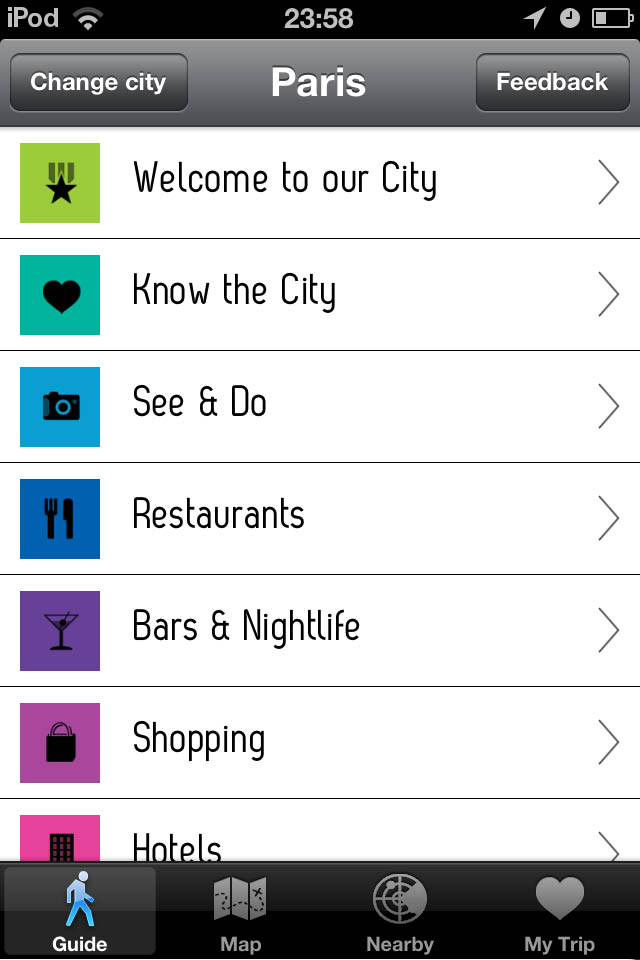
\includegraphics[height=7.5cm]{./images/screenshots/screenshot_guidepal_1.jpg}
                \caption{Category selection for filtering the locations.}
                \label{fig:guidePalCategorySelection}
        \end{subfigure}%
        \quad\quad\quad\quad\quad
        \begin{subfigure}[b]{0.25\textwidth}
                \centering
                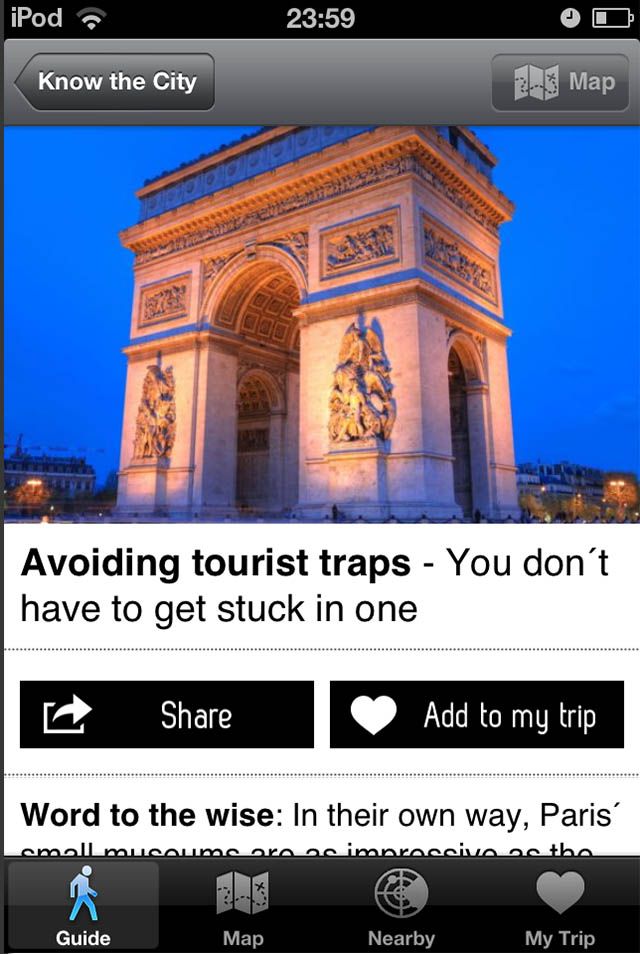
\includegraphics[height=7.5cm]{./images/screenshots/screenshot_guidepal_2.jpg}
                \caption{Detailed information about touristic location.}
                \label{fig:guidePalDetailedInformation}
        \end{subfigure}
        \caption{GuidePal~\cite{GuidePalWeb}\cite{GuidePaliPhone} iPhone application screenshots.}
        \label{fig:guidePalIphoneScreenshots}
\end{figure}
\\
In order to list the existing points of interest, the user selects the desired city and category as illustrated by  Figure~\ref{fig:guidePalIphoneScreenshots}~(\subref{fig:guidePalCategorySelection}). After selecting the intended category, a description for the point of interest is presented; Figure~\ref{fig:guidePalIphoneScreenshots}~(\subref{fig:guidePalDetailedInformation}) shows the selection of the "Know the City" category.\\
\\
This application also have some augmented reality features, providing users with the possibility to map the real world (captured by the camera of the device) with the touristic attractions in real time. When the camera points to the direction where touristic locations are available near by, those are presented above the image. By selecting any of the presented locations, the user is redirected to the detail page similar to one illustrated on Figure~\ref{fig:guidePalIphoneScreenshots}~(\subref{fig:guidePalDetailedInformation}).
%%%%%%%%
\subsection{mTrip}
mTrip~\cite{mTrip} travel guide service is mainly used for big cities such as Paris, Berlin,  Madrid, and others. It is available as a separate application for each one of the major cities (for both iPhone and Android) and allows people to consult information regarding points of interest without an Internet connection. Figure~\ref{fig:mtripScreenshots} presents some screenshots of this application. \\
\\
Users can plan an itinerary or create guides for the cities by providing the detailed information on the touristic attractions they plan to visit. After specifying the dates for the trip, each user can manually compose his itinerary or allow mTrip to automatically generate an itinerary for the trip. When the automatic mode is chosen, one must indicate preferences for the attractions to be visited, as shown on Figure~\ref{fig:mtripScreenshots}~(\subref{fig:mTripPreferencesCustomization}). A list of points of interest is presented when the user selects a specific category, similar to those shown on Figure~\ref{fig:mtripScreenshots}~(\subref{fig:mTripTouisticLocations}).
\\
%%%%%%%%%%%%%%%%%
\begin{figure}
        \centering
        \begin{subfigure}[b]{0.25\textwidth}
                \centering
                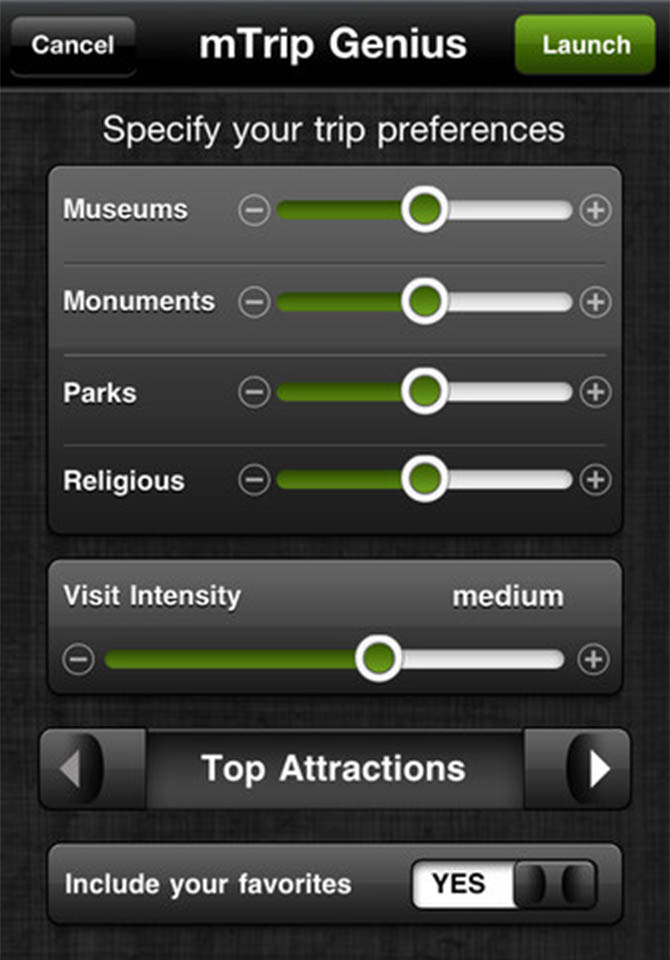
\includegraphics[height=7.5cm]{./images/screenshots/screenshot_mtrip_1.jpg}
                \caption{Customization of the itinerary.}
                \label{fig:mTripPreferencesCustomization}
        \end{subfigure}%
        \quad\quad\quad\quad\quad\quad
        \begin{subfigure}[b]{0.25\textwidth}
                \centering
                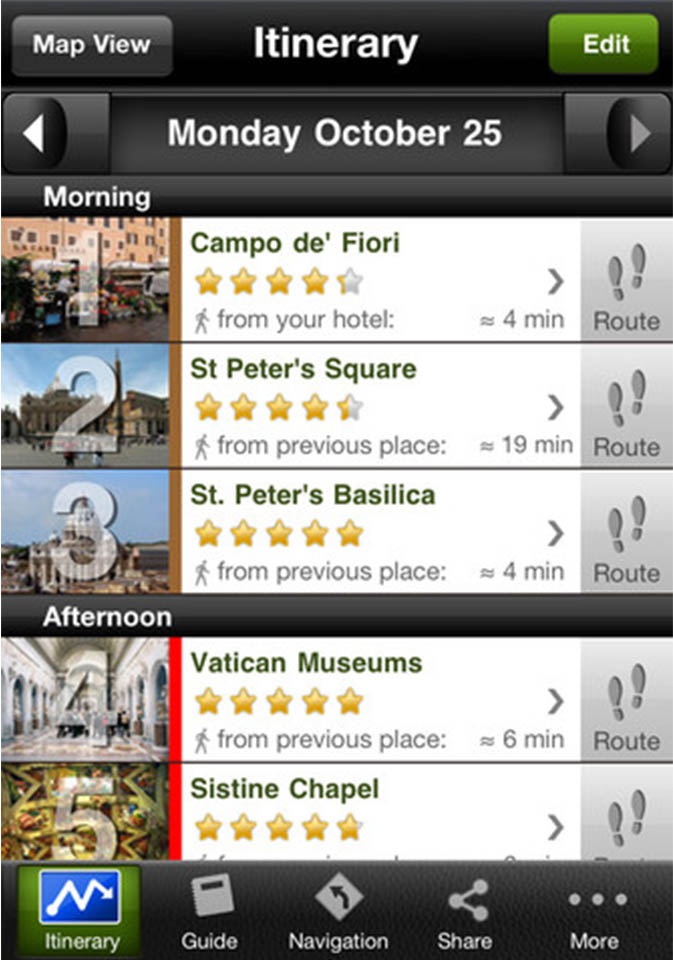
\includegraphics[height=7.5cm]{./images/screenshots/screenshot_mtrip_2.jpg}
                \caption{List of the touristic locations.}
                \label{fig:mTripTouisticLocations}
        \end{subfigure}
        \caption{mTrip iPhone application screenshots.}
        \label{fig:mtripScreenshots}
\end{figure}
\\
%%%%%%%%%%%%%%%%%
Each point of interest is accompanied by a description, a photo, opening hour, prices, as well as the comments and ratings from other travellers. The application provides an augmented reality tool that allows to preview of the points of interest around the user's current location.
%%%%%%%%
\subsection{Triposo}
Triposo~\cite{triposo} shares similar concepts with the mTrip application. However, it includes much more countries as well as smaller cities. When one picks the country to visit, the download of information regarding the points of interest for that country starts immediately, allowing to consult this information later in offline mode. Some major cities require additional downloads due to the large amount of the points of interest and touristic attractions. For big cities, users have access to special information regarding the city guide about all sights, a list of restaurants and extended nightlife options. The application also offers a travel dashboard with currency converter, weather, and useful native language phrases. Triposo uses freely available content from different sources, such as Wikipedia~\cite{wikipedia}, Wikitravel~\cite{wikitravel}, World66~\cite{world66}, among others.\\
\\
As it is shown by the screenshot on Figure~\ref{fig:triposoScreenshots}~(\subref{fig:triposoSuggestedPointsOfInterest}), a set of suggested points of interest for Lisbon is presented along with the main navigation items. Figure~\ref{fig:triposoScreenshots}~(\subref{fig:triposoWeahtherTime}) shows the current weather and current time for Porto as well as the spelling of some Portuguese words.\\
%%%%%%%%%%
\begin{figure}
        \centering
        \begin{subfigure}[b]{0.25\textwidth}
                \centering
                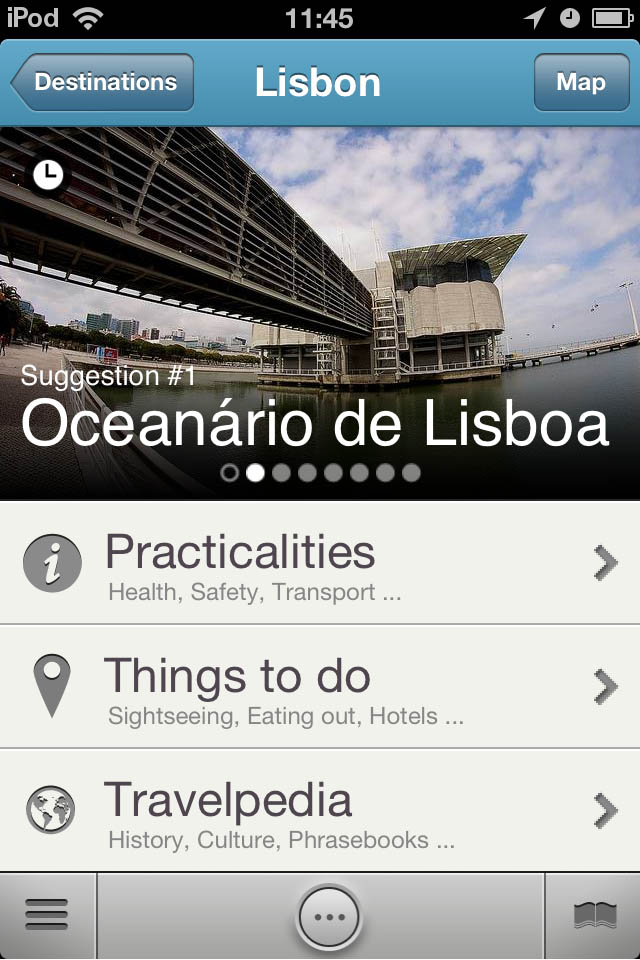
\includegraphics[height=7.5cm]{./images/screenshots/screenshot_triposo_1.jpg}
                \caption{Suggested points of interest.}
                \label{fig:triposoSuggestedPointsOfInterest}
        \end{subfigure}%
        \quad\quad\quad\quad\quad
        \begin{subfigure}[b]{0.25\textwidth}
                \centering
                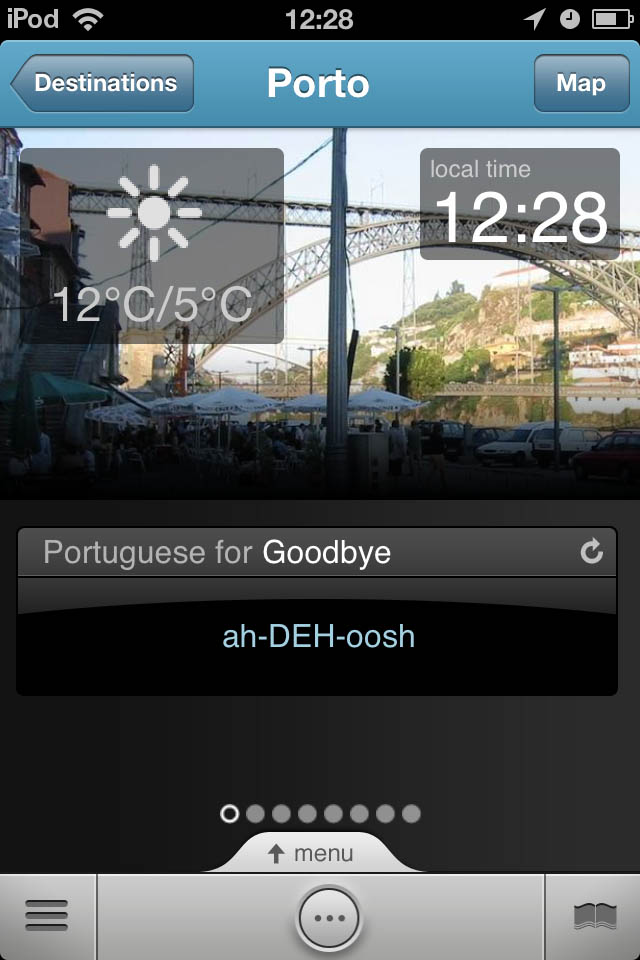
\includegraphics[height=7.5cm]{./images/screenshots/screenshot_triposo_2.jpg}
                \caption{Shortcuts and useful information.}
                \label{fig:triposoWeahtherTime}
        \end{subfigure}%
        \caption{Triposo iPhone application screenshots.}
        \label{fig:triposoScreenshots}
\end{figure}


%%%%%%%%%%
\subsection{Foursquare}
Foursquare is a service that allows registered users to "check-in\footnote{Check-in refers to the user's action for posting his current location at a venue.}" at their current location. It is composed by both web and mobile applications for iPhone, Android and Blackberry. Users with special permission have the possibility to contribute with new locations, such as coffee shops, restaurants, sights, among others. The service was created in 2009 and in March of 2011 a new version with a recommendation engine~\cite{foursqureRecommendationEngine} was developed, for suggesting places that users might like, based on their past actions.\\
\\
In 2013 an updated version of the service was launched, where users can consult the sights nearby their current location. The map view with the recommended sights nearby users current location is shown on Figure~\ref{fig:4SqureScreenshots}~(\subref{fig:4squre2}). An example of the touristic location details is shown on Figure~\ref{fig:4SqureScreenshots}~(\subref{fig:4squre3}) where user can have the preview of the location, save it to favourites, perform the check in, among others.\\
\\
\begin{figure}
        \centering
        \begin{subfigure}[b]{0.25\textwidth}
                \centering
                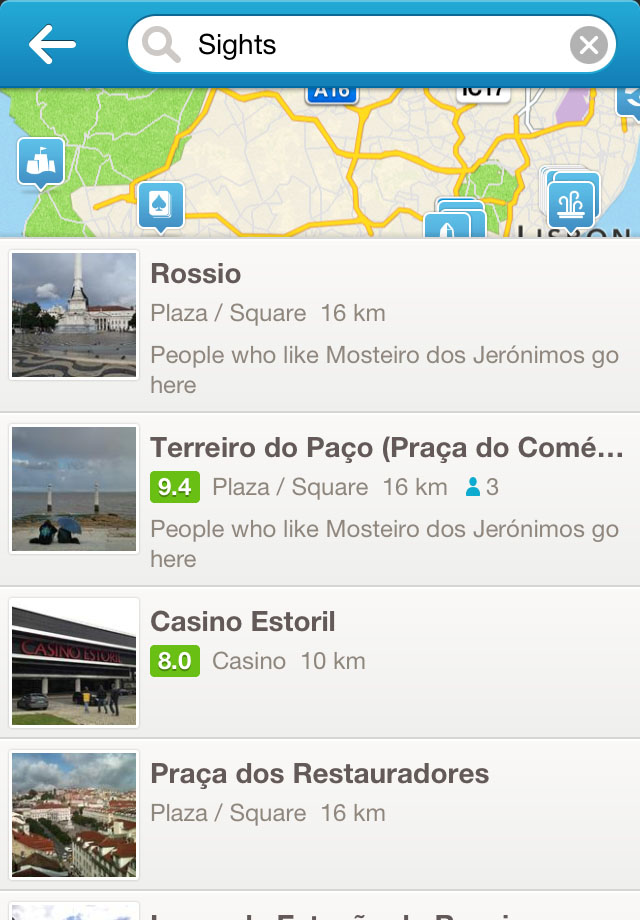
\includegraphics[height=7cm]{./images/screenshots/screenshot_foursqure_1.jpg}
                \caption{Map view with sights nearby user's location.}
                \label{fig:4squre2}
        \end{subfigure}%
        \quad\quad\quad\quad\quad
        \begin{subfigure}[b]{0.25\textwidth}
                \centering
                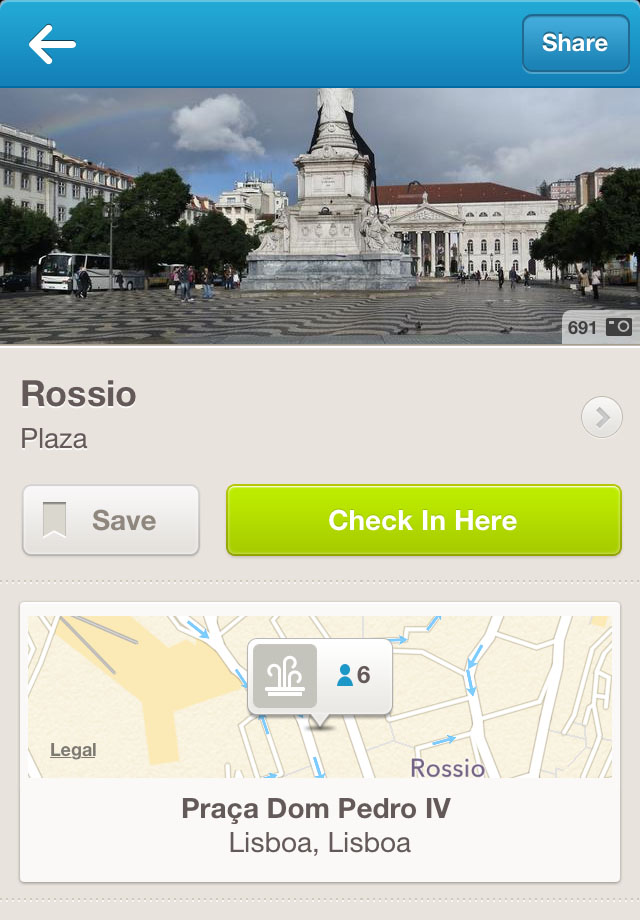
\includegraphics[height=7cm]{./images/screenshots/screenshot_foursqure_2.jpg}
                \caption{Details of the Touristic location.}
                \label{fig:4squre3}
        \end{subfigure}%
        \caption{Foursquare iPhone application screenshots.}
        \label{fig:4SqureScreenshots}
\end{figure}
\\
All these applications are modern solutions for tourist guides. The Foursquare service was created in 2009, the mTrip and TouristEye in 2010, whereas the Triposo and GuidePal have been published in 2011. 
\newpage

\section{Proposed Solution}
\label{sec:ftbd}
This Section introduces the simplified service architecture as well as the employed technologies used during the development of the system components. The system is mainly composed by the~\gls{rest}~\cite{RestWebber} service with a data access layer which exposes a set of endpoints\footnote{In \gls{soa}, an endpoint is the entry point to a service.} accessible by the client applications. Client applications are available as Web-based and Mobile (for iOS~\cite{ios} platforms iPhone and iPad). Figure~\ref{fig:introductioArchitecture} shows the proposed service architecture.\\
\\
\begin{figure}[h!]
 \centering
   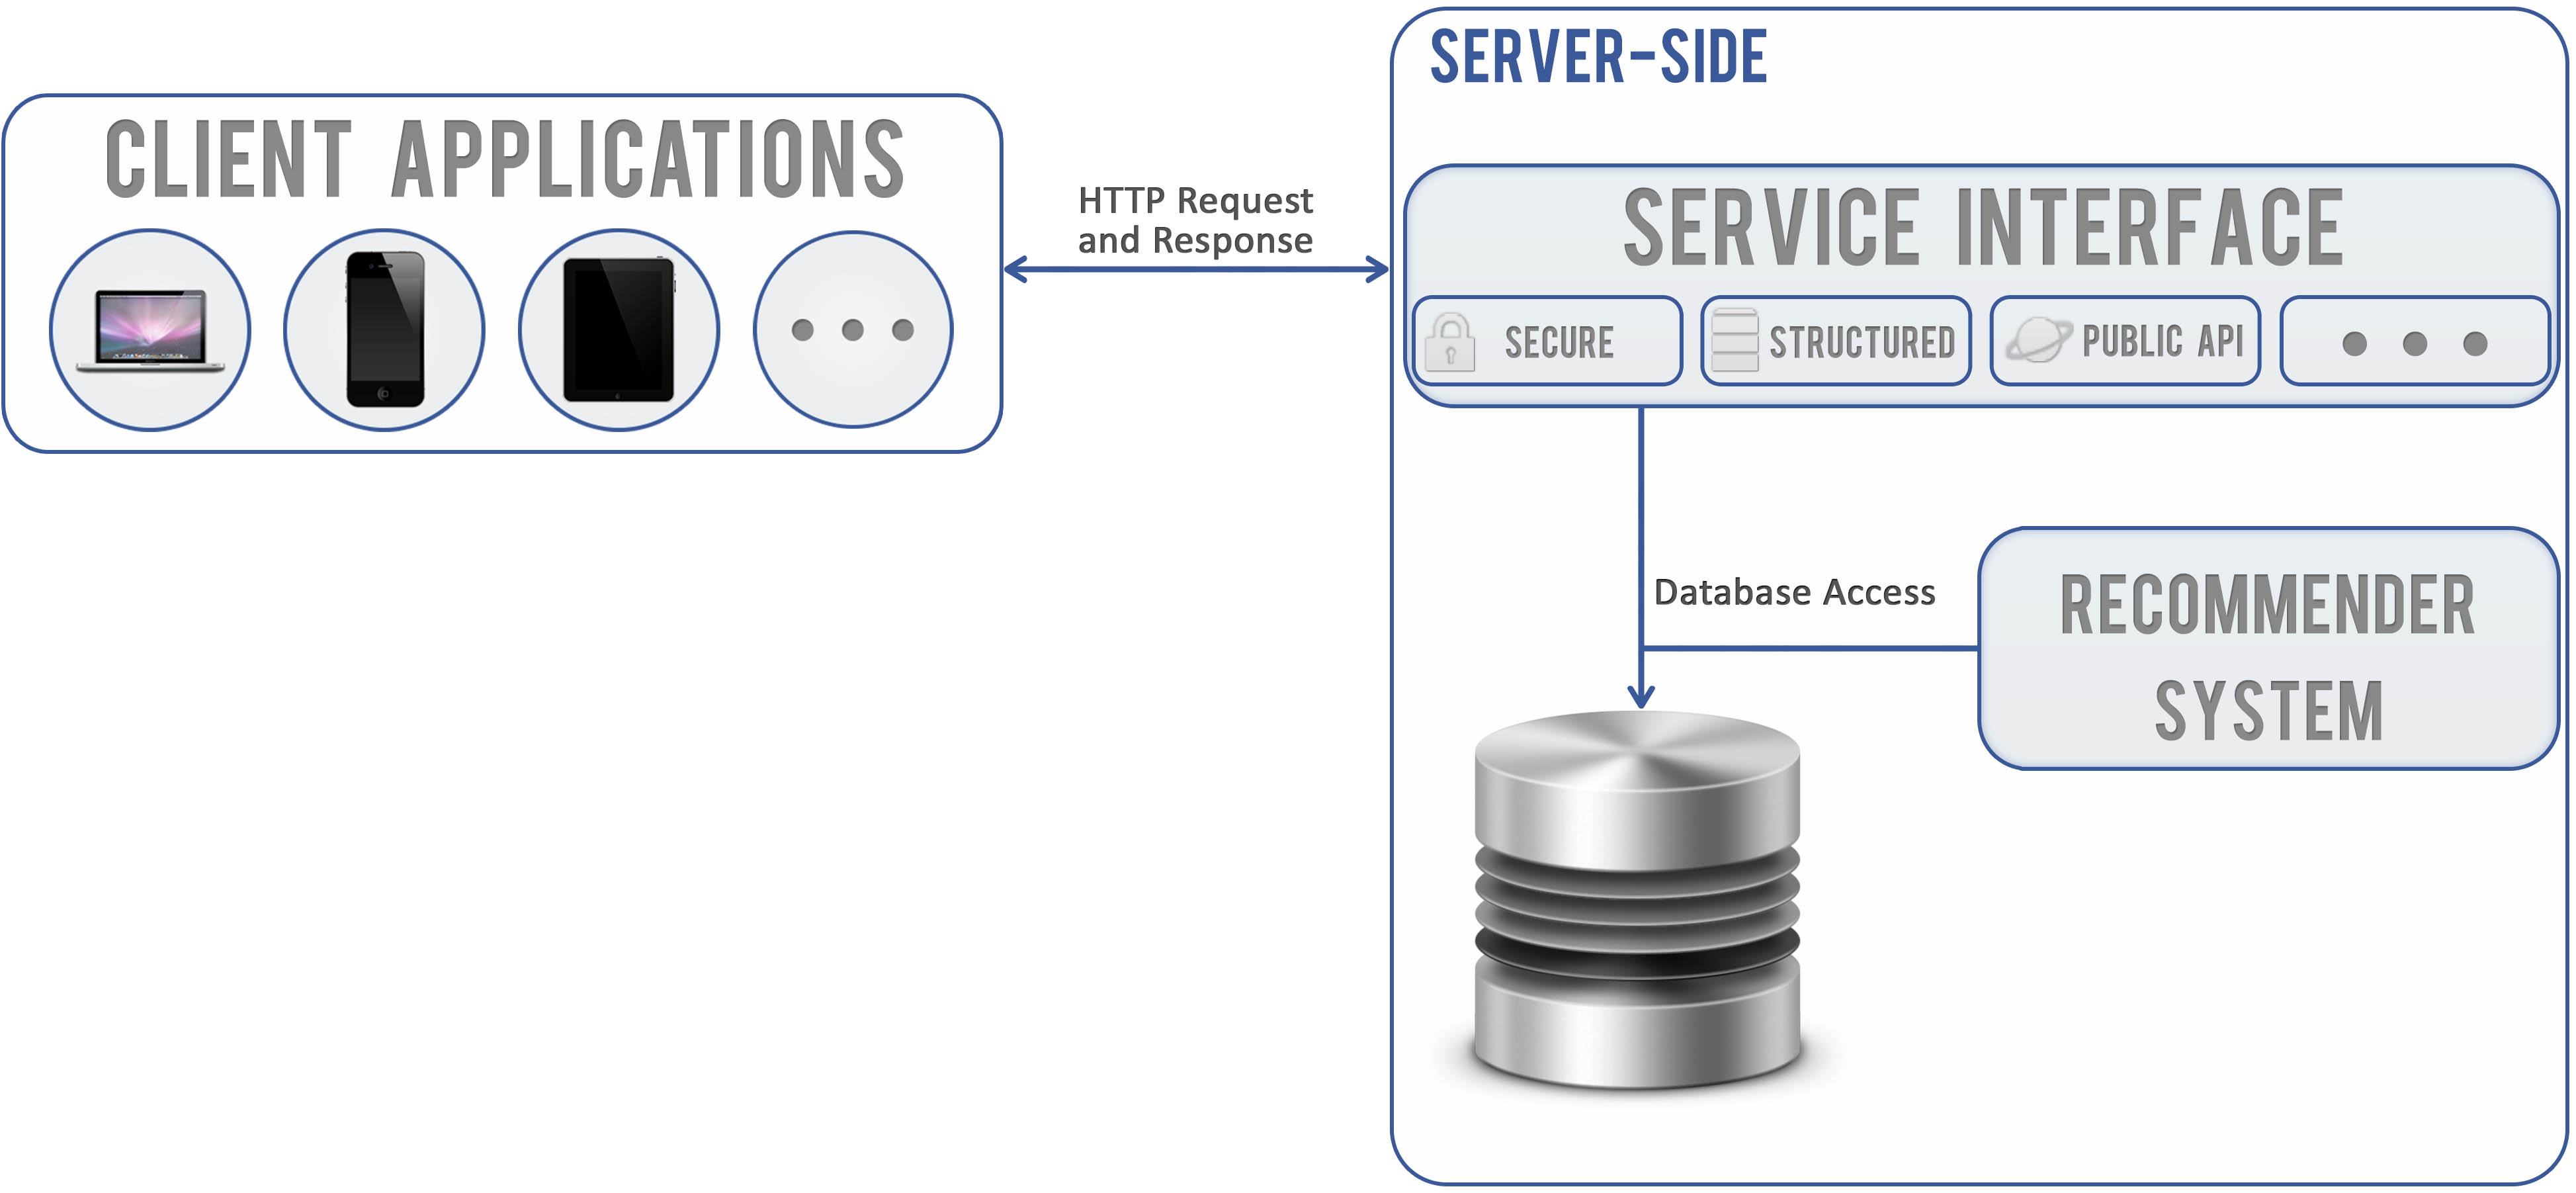
\includegraphics[width=14.8 cm]{./images/diagrams/diagram_introduction_architecture.jpg}
   \caption{Generic service architecture.}
   \label{fig:introductioArchitecture}
\end{figure}\\
\\
The service is divided into four main layers, with the following roles:
\begin{itemize}
 \item The Database layer stores information regarding points of interest, user data, among other types of data.
 \item The Service Interface is responsible for communicating with the Database layer. It makes all accesses transparent to the end client applications. This layer is mainly responsible for the data security and integrity, delivery of information in structured format, among others.
 \item The Recommender System is responsible for finding new points of interest based on the user's past actions, and to recommend these to the user. This service uses data from the database layer in order to compute recommendations.
 \item Client Applications make \gls{http} requests in order to access data from the public \gls{api}, provided by the Service Interface layer.
\end{itemize}

\subsection{Tools and Technologies}
\label{subsec:ttbuipd}
This Subsection introduces the technologies and tools used to achieve the goals of this project. We begin by describing a set of technologies related to databases, data model, and the \gls{rest} service. Then, the Web related technologies are discussed and finally we address the mobile applications.\\
\\
%%%%
For information storage, we use the MySQL~\cite{MySqlOrcale} relational database, which uses the \gls{sql} for accessing and manipulating databases. In order to facilitate the service development process, a pre-populated database was created with a few tens of points of interest.\\
\\
%%%%
The \gls{rest}~\gls{api} is developed in order to provide a single data source for client applications, including those already developed within this project and others that may appear in the future. The \gls{api} is implemented using the Java environment and Play~Framework~\cite{playFramework}.\\
\\
The Web application implementation is focused in technologies for user interface definition and structuring such as~\gls{html5}~\cite{html5},~\gls{css3}~\cite{css3} and also the JavaScript~\cite{javaScript} technology to enrich user's interactivity. The server side of the web application was developed using the Play Framework. Twitter Bootstrap~\cite{twitterBootstrap} framework was used to generate the layout with desired dynamic content, thus providing an user friendly platform.\\
\\
%\marginpar{} %%%
In the past few years, mobile devices have been used and widespread with great success, starting with Apple's iPhone launch and later with the iPad~\cite{iPadSanchez}. Both devices share the same operating system named iOS that offers a development platform for object-oriented applications. Those are written in Objective-C~\cite{ObjectiveC}\footnote{The Objective-C is a computer programming language based on C and Smalltalk. It is designed to leverage the C language with full object-oriented programming capability, through the mechanism of message passing. When in Objective-C one sends a message, its target is resolved at runtime and then it interprets the message with the receiving object~\cite{ObjectiveC}~\cite{objectiveCBook}.} using the iOS SDK (Software Development Kit). In the course of this project the targeted applications were designed taking into consideration advanced aspects of the iOS platform such as sharing code between iPhone and iPad, by means of an Universal Application~\cite{UniversalApps}.\\
\\
%\marginpar{} %%%
The development of these applications was carried out using the \gls{ide} Xcode~\cite{Xcode}.

\subsection{Core Features}
\label{subsec:cf}
This Subsection contains a description of the core features provided by the service, which are presented in Table~\ref{tab:coreFeatures}.\\
\\
\newpage
\begin{center}
    \begin{longtable}{ | p{3.5cm} | p{11.1cm} |}
    \caption{Core features of the GuideMe service.}
    \label{tab:coreFeatures}
	\\
    \hline
    \textbf{Feature Name} & \textbf{Description}\\ \hline
    \hline
    \specialcell[t]{Internationalization\\support} & 
    The aim of the project is to support points of interest of Portugal, but its architecture is designed in order to easily be expanded and to support other countries. Multilingual support is implemented for the database, REST API and application levels. \\ 
    \hline
    
    Filtering options &
    The following features are supported:
	\begin{itemize}
	\item lookup for points of interest nearby the user's current location;
	\item filtering of the locations based on the following characteristics:
	\begin{itemize}
		\item specific attraction;
		\item user's current location, by using the geographic coordinates retrieved from the mobile device;
		\item time that the user can spend;
		\item time of day of the visit;
		\item preferred weather conditions.
	\end{itemize}
	\item places that can be visited under given weather conditions such as rainy or sunny days, among others. It requires integration with the \gls{wwo} meteorology~\gls{api}, in order to advise or not the visit to the chosen user location;
	\item filtering by the maximum distance to the point of interest, based on the user's current location and mobility.
	\end{itemize}
    \\ 
    \hline
    
    \specialcell[t]{Wanted and\\already seen} &
	Users have the possibility to create a list of locations that they intend to visit as well as access the history of already visited locations. \\ 
    \hline

	\specialcell[t]{Social component} &
    	The following features are supported:
	\begin{itemize}
	\item Integration with social networks in order to encourage users to share visits with their friends;
	\item Based on the visits and mutual preferences between various users, the system recommends new places to visit that users may like. The recommendations are produced by the recommender system, using Collaborative Filtering (CF)~\cite{ibCollabrativeVSGK}\cite{AmazonRecommendGLBSJY}\cite{recommSystemPMVS} algorithms. The proposed solution is further explained in Section~\ref{sec:ocft};
	\item The service implements the social component by itself, providing the concept of the \emph{Following} and \emph{Follower} in order to establish friendship between users. Users are notified about certain actions performed by their friends.
	\end{itemize}
    \\ 
    \hline
    
    Notification system &
    Users can receive push notifications on their iOS device when someone has started to follow them. These notifications are carried out using the~\gls{apns}~\cite{apns}.\\
\hline
    
   	Login and sign up &
    Authentication and sign up through the most popular social network services, such as Facebook~\cite{FacebookLogin} and Twitter~\cite{TwitterLogin}. \\
    \hline
    
   	Back office &
    The iOS applications implements a back office system where privileged users can create or edit an existing location. They have permission to consult log information of the different service components, to analyse and correct information regarding the touristic location that were reported by other users.\\
\hline

   	Near by  &
    Preview of the sights, near by user's geographic locations. The use-case of this feature is illustrated on Figure~\ref{fig:useCaseFilterByLocation}.\\
\hline

   	Recommended touristic locations  &
	The service performs recommendation of the touristic locations to users, based on their past visits. The detailed illustration of this scenario is shown on Figure~\ref{fig:useCaseRecommendationLocation}.\\
\hline
    \end{longtable}
\end{center}
%%%%%%%%%%%%%%%%%%%%
The use-case illustrated on Figure~\ref{fig:useCaseFilterByLocation} consists in providing the user with information regarding the sights near by his/her current location.\\
%%%%%%%%%%%%%%%%%%%%
\begin{figure}[h!]
 \centering
   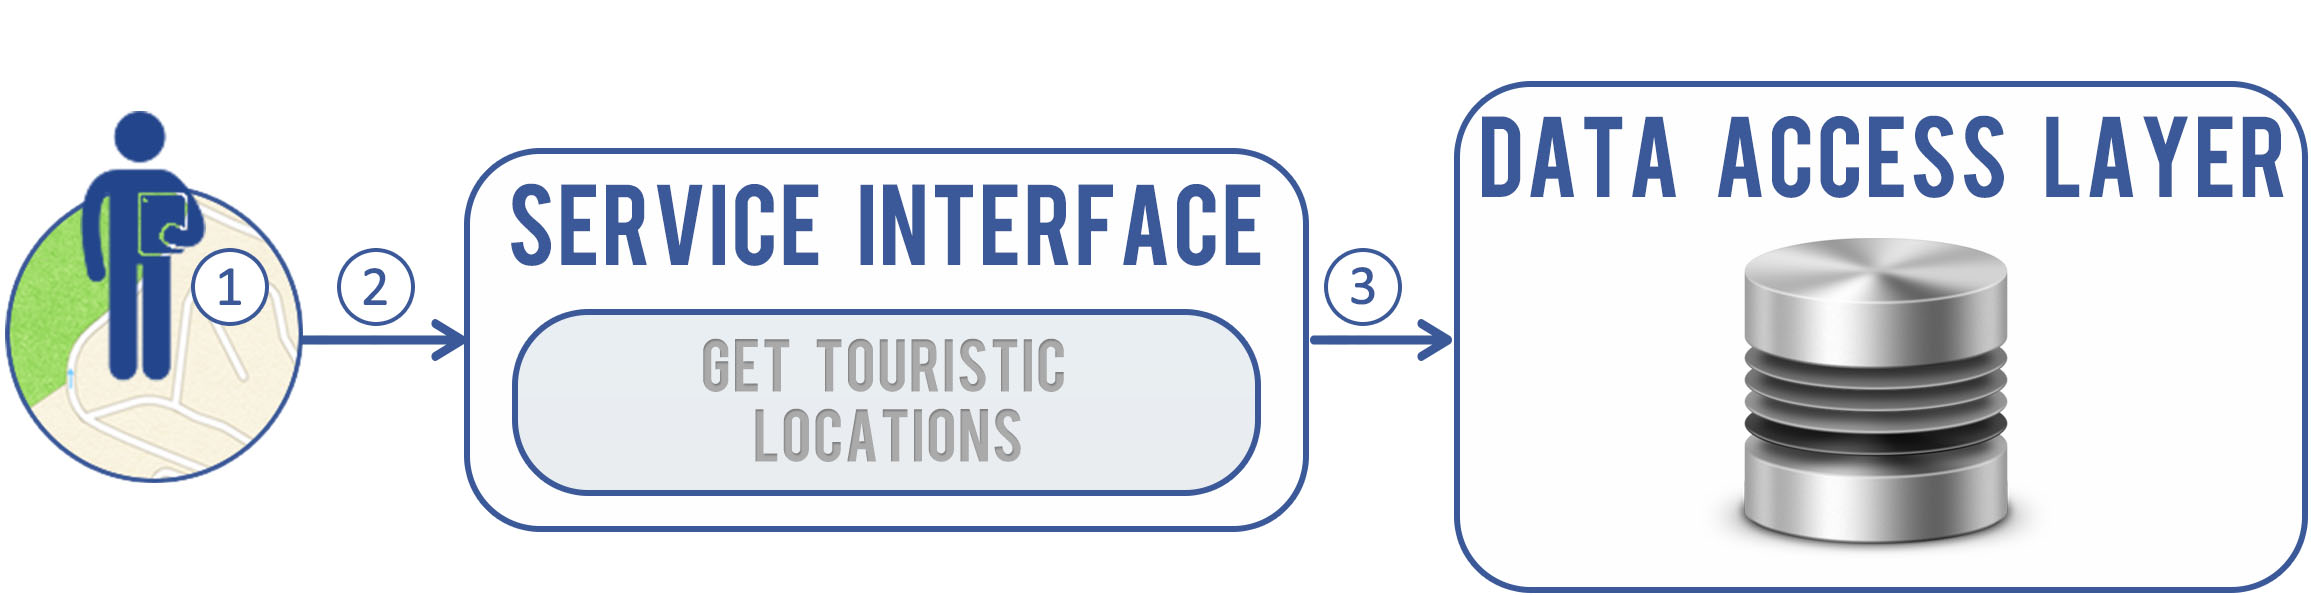
\includegraphics[width=13.0 cm]{./images/diagrams/diagram_usecase_users_location.jpg}
   \caption{Use-case of the near by feature.}
   \label{fig:useCaseFilterByLocation}
\end{figure}\\
%%%%%%%%%%%%%%%%%%%%
Each step is detailed as follows:
\begin{enumerate}
\item The geographic coordinates of user's current location, are obtained through the ~\gls{gps} of the mobile device.
\item Through the service interface, users make the requests to obtain the touristic locations passing the previously obtained geographic coordinates.
\item The service interface interacts with the Data Access Layer (DAL) in order to list the touristic locations. The distance is calculated between each sight and the submitted geographic coordinates, providing the results sorted in ascending order of distance.
\end{enumerate}
%%%%%%%%%%%%%%%%%%%%
The recommender system is one of the most important features of the developed service. The summarised process of the recommendation system is illustrated on Figure~\ref{fig:useCaseRecommendationLocation}.\\
%%%%%%%%%%%%%%%%%%%%
\begin{figure}[h!]
 \centering
   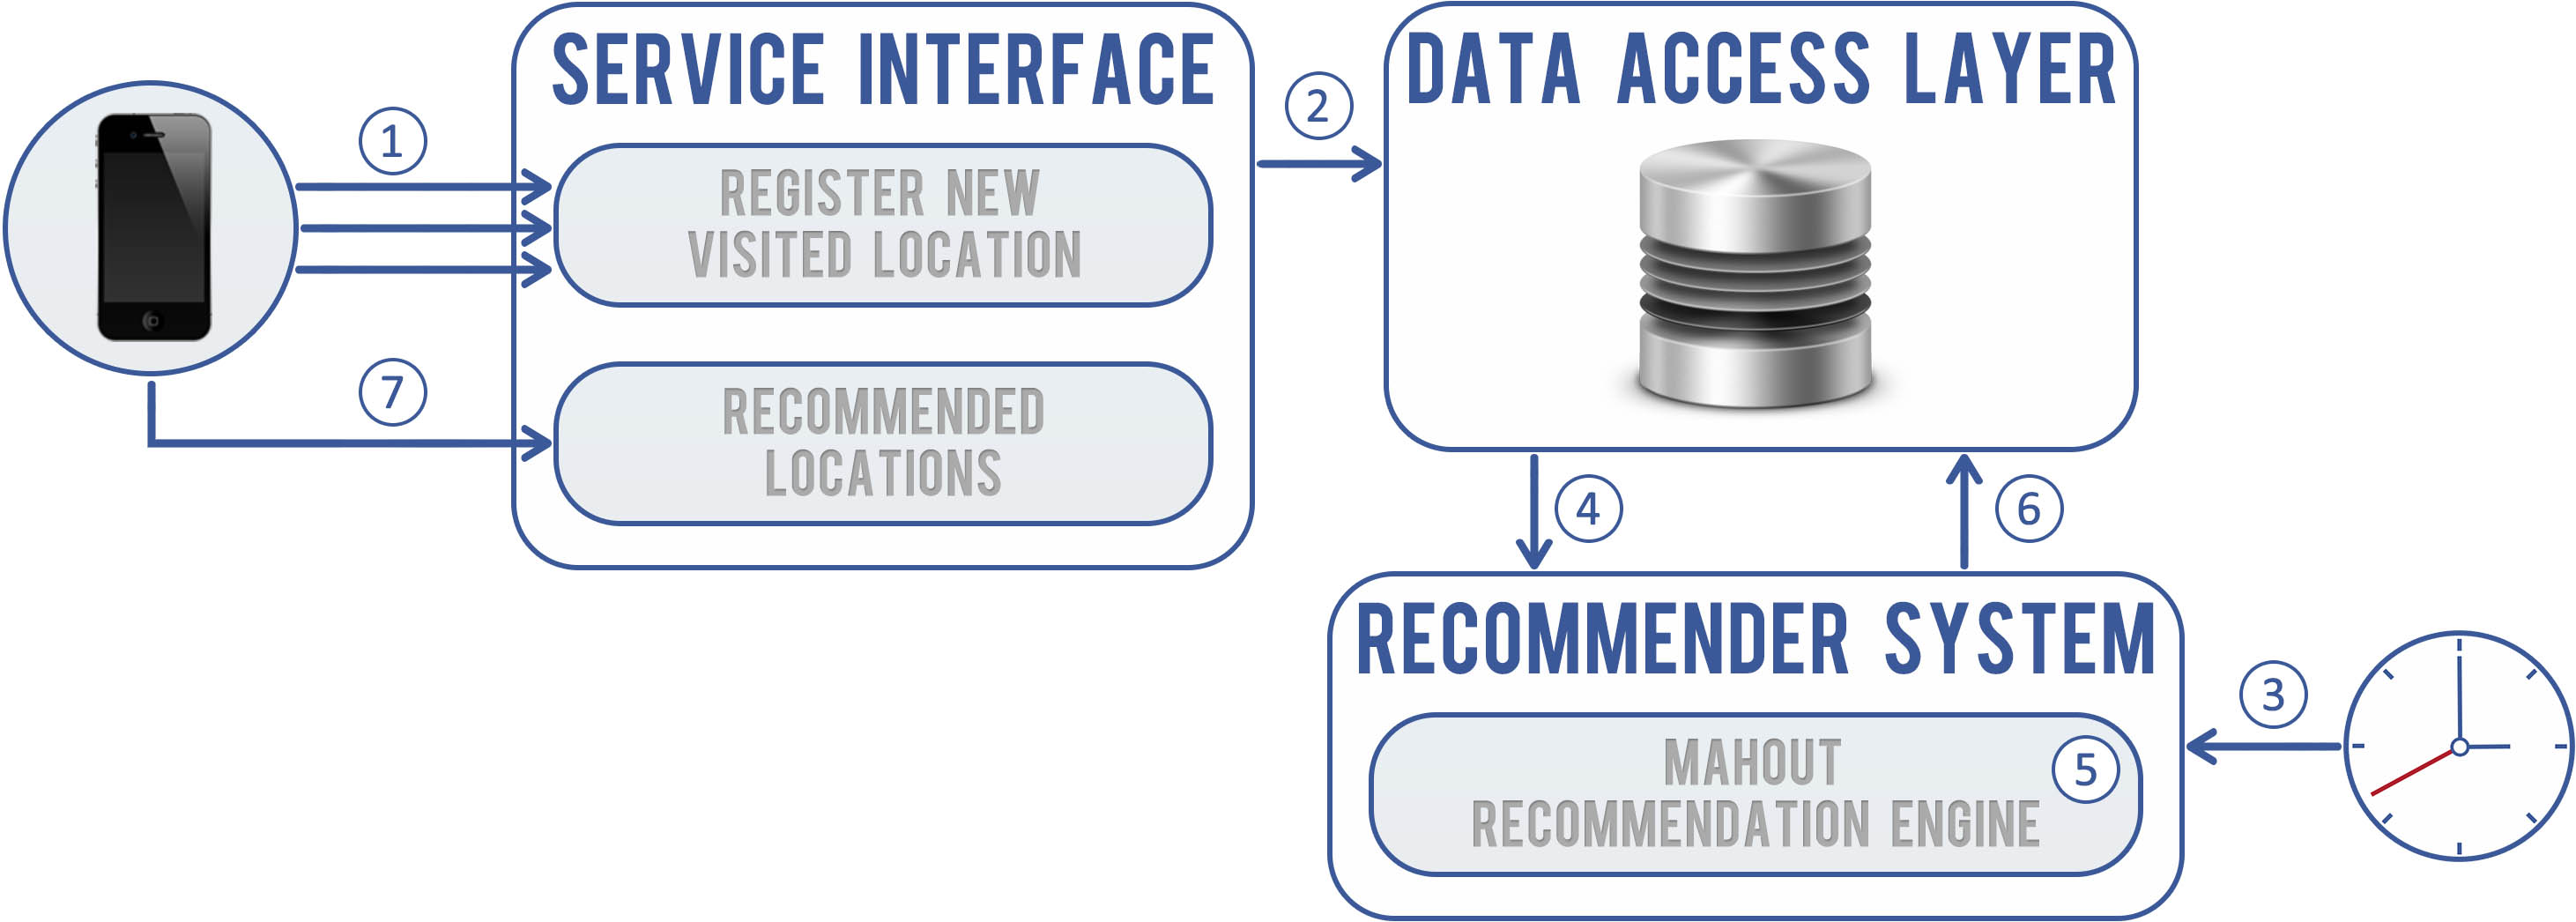
\includegraphics[width=13.0 cm]{./images/diagrams/diagram_usecase_recommender_system.jpg}
   \caption{The recommendation process.}
   \label{fig:useCaseRecommendationLocation}
\end{figure}\\
The full process of the recommendation system is as follows:
\begin{enumerate}
\item Through the service interface, the user marks new locations as visited.
\item Using the implemented DAL, the information is stored into the database.
\item The Cron Job\footnote{Cron is a time-based job scheduler in Unix-like computer operating systems.}~\cite{cronTab} is triggered everyday at 3:00 A.M., performing the recommendation process.
\item The recommender system obtains users eligible for the new recommendations.
\item For each user, the recommender system computes a set of locations previously unseen by the user.
\item Through the DAL, the recommender service removes previous recommendations and populates the database with the new information.
\item Later, the user obtains a list of recommendations through the service interface.
\end{enumerate}
%%%%%%%%%%%%%%%%%%%%
When comparing the GuideMe service with similar applications reviewed in Section~\ref{sec:sota}, it offers:
\begin{itemize}
	\item filters of unique kind that allow searching for points of interest;
	\item a friendly and usable interface for both Web and mobile applications;
	\item integration with algorithms and services that minimize human interaction during the approval process of newly inserted locations.
\end{itemize}

\section{Report Organization}
\label{sec:reportOrganization}
The remainder of this report is organized as follows. In Chapter~\ref{theory}, we introduce the background concepts and terminology of the recommender system and different collaborative filtering techniques. Chapter~\ref{implementation} approaches the proposed solution by detailing: the chosen service architecture, the integration with the~\gls{apns} service, the analysis of different frameworks for the implementation of the~\gls{dal}, and the~\gls{rest}~\gls{api}. Chapter~\ref{implementation} also includes prototypes that were initially designed before the development of the client applications.\\
\\
In Chapter~\ref{developed-work}, we describe all the developments that were made for making this project a reality. In detail, this Chapter describes the implementation aspects of the database models for both Service and Log databases, structure of the the~\gls{rest}~\gls{api} endpoints, different characteristics of the implemented recommender system, and push notification provider. We introduce the main features, as also some implementation details of the web and iOS applications. Chapter~\ref{chapter:expRsults} is devoted to the experimental results, which have guided the implementations in the correct direction. This Chapter reflects an analysis of the different recommendation system algorithms and load tests.\\
\\
We end the document with the Chapter~\ref{conclusions} by detailing the core aspects of the project and the fulfilled objectives. In order to make the service more usable and robust, as future work we present some points that should be improved in terms of security and functionalities.

\section{Our Contribution}
\label{sec:ourContribution}
We've recently submitted an article~\cite{guideMeArticle} to the 2013 Conference on Electronics, Telecommunications and Computers (CETC 2013), where we describe the main parts of this work. We believe that the developed project contribute to the evolution of tourist guide services, and promotes the effective integration of recommendation systems as a tool to easily find new interesting places to visit.
\fi

\chapter{State-of-the-Art}
\label{stateofart}
\thispagestyle{plain}

In this section, we review the state-of-the-art of the problem at hand. We start by describing why timetabling is a rather complex problem, some possible approaches to solve it and some of the existing solutions, specifically for the \gls{itc2007} benchmarks.\\

\section{Timetabling Problem}

When solving timetabling problems, it is possible to generate one of multiple types of solutions which are: \textit{feasible}, \textit{non feasible}, \textit{optimal} or \textit{sub-optimal}. A feasible solution solves all the mandatory constraints, unlike non feasible solutions. An optimal solution is the best possible feasible solution given the problem constraints. A problem may have multiple optimal solutions. Lastly, non-optimal solutions are feasible solutions that have sub-optimal values.\\
\\
Timetabling automation is a subject that has been a target of research for about 50 years. The timetabling problem may be formulated as a search or an optimization problem \cite{Schaerf1999}. As a search problem, the goal consists on finding a feasible solution that satisfies all the hard constraints, while ignoring the soft constraints. By posing the timetabling problem as an optimization problem, one seeks to minimize the violations of soft constraints while satisfying the hard constraints. Typically, the optimization is done after the use of a search procedure for finding an initial feasible solution.\\
\\
The basic examination timetabling problem, where only the \textit{clash} hard constraint is observed, reduces to the graph coloring problem~\cite{Jensen2001}, which is a well studied problem. The clash hard constraint specifies that no conflicting exams should be scheduled at the same time slot. Deciding whether a solution exists in the graph coloring problem, is a NP-complete \cite{Arora2009} problem \cite{Qu2009}. Considering the graph coloring as an optimization problem, it is proven that the task of finding the optimal solution is also a NP-Hard \cite{Arora2009} problem \cite{Qu2009}. Graph Coloring problems are explained further in Section \ref{section:existingappr}
\\
%%%%%%%%%%%%%%%%%%%%
\section{Existing Approaches}
\label{section:existingappr}
%%%%%%%%%%%%%%%%%%%%
\begin{figure}[t!]
 \centering
   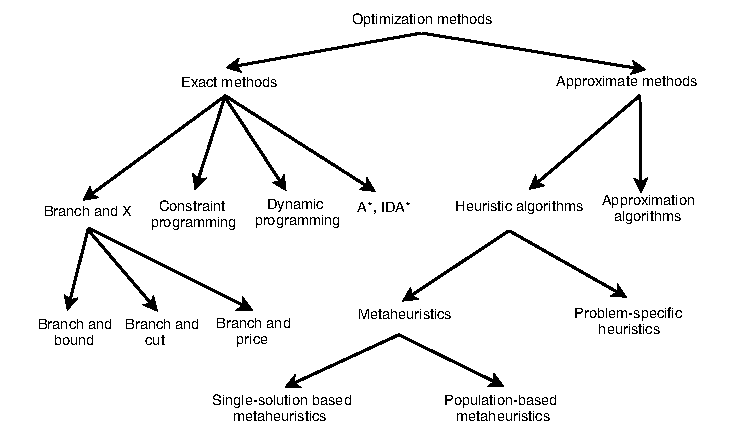
\includegraphics[width=1\textwidth,natwidth=1317,natheight=814]{./images/typesOfAlgorithms.pdf}
   \caption{Optimization methods: taxonomy and organization (adapted from \cite{Talbi2009}).}
   \label{fig:TypesAlgorithms}
\end{figure}

Figure~\ref{fig:TypesAlgorithms} depicts a taxonomy for the known optimization methods. These methods are divided into \textit{Exact methods} and \textit{Approximate methods}.\\
\\
Timetabling solution approaches are usually divided into the following categories~\cite{Qu2009}: \textit{exact algorithms} (Branch-and-Bound, Constraint Programming), \textit{graph based sequential techniques}, \textit{Single-solution based meta-heuristics} (Tabu Search, Simulated Annealing, Great Deluge), \textit{population based algorithms} (Evolutionary Algorithms, Memetic algorithms, Ant Colony algorithms, Artificial immune algorithms), \textit{Multi-criteria techniques}, \textit{Hyper-heuristics}, and \textit{Decomposition/clustering techniques}. Hybrid algorithms, which combine features of several algorithms, comprise the state-of-the-art. Due to its complexity, approaching the examination timetabling problem using exact method approaches can only be done for small size instances. Real problem instances found in practice are usually of large size, making the use of exact methods impracticable. Heuristic solution algorithms have been usually employed to solve this problem.\\
\\
Real problem instances are usually solved by applying algorithms which use both \textit{heuristics} and \textit{meta-heuristics}. Heuristic algorithms are problem-dependent, meaning that these are adapted to a specific problem in which one can take advantage of its details. Heuristics are usually used to obtain a solution (feasible or not). For example, graph-coloring heuristics are used to obtain solutions for a given timetable problem instance. Usually only the hard constraints are considered in this phase. Meta-heuristics, on the other hand, are problem-independent, and are used to optimize any type problem. In these, one usually consider both hard and soft requirements.\\
\\
Most of the existing meta-heuristic algorithms belong to one of the following three categories: One-Stage algorithms, Two-Stage algorithms and algorithms that allow relaxations~\cite{Lewis2007}. The One-Stage algorithm is used to get a solution, which the goal is to satisfy both hard and soft constraints at the same time. The Two-Stage algorithms are the most used types of approaches. This category is divided in two phases: the first phase consists in not considering the soft constraints and focusing on solving hard constraints to obtain a feasible solution; the second phase is an attempt to find the best solution, trying to solve the largest number of soft constraints as possible, given the solution of the first phase. Algorithms that allow relaxation can weaken some constraints in order to solve the \textit{relaxed problem}, while considering the satisfaction of the original constraints that were weakened, on a later stage of the algorithm.

\subsection{Exact methods}
\label{subsection:exactmethods}
Approximation algorithms like heuristics and meta-heuristics proceed to enumerate partially the search space and, for that reason, they can't guarantee finding the optimal solution. Exact approaches perform an implicit enumeration of the search space and thus guarantee that the encountered solution is optimal. A negative aspect is the time taken to find the solution. If the decision problem is very difficult (e.g., NP-Complete), in practical scenarios, given large size problem instances, it may not be possible to use this approach due to the long execution time.\\

\subsubsection{Constraint-Programming Based Technique}
The gls{cpbt} allows direct programming with constraints which gives ease and flexibility in solving problems like timetabling. Two important features about this technique are the use of backtracking and logical variables. Constraint programming is different from other types of programming, as in these types it is specified the steps that need to be executed, but in constraint programming only the properties (hard constraints) of the solution, or the properties that should not be in the solution, are specified \cite{Qu2009}.\\

\subsubsection{Integer Programming}
The \gls{ip} is a mathematical programming technique in which the optimization problem to be solved must be formulated as an Integer Problem. If the objective function and the constraints must be linear, and all problem variables are integer valued, then the \gls{ip} problem is termed \gls{ilp}. In the presence of both integer and continuous variables, then the problem is called \gls{milp}. Schaerf~\cite{Schaerf1999} surveys some approaches using the \gls{milp} technique to school, course, and examination timetabling.\\

\subsection{Graph Coloring Based Techniques}
\label{subsection:graphcoloring}
As mentioned previously, timetabling problems can be reduced to a graph coloring problem. Considering this relation between the two problems, several authors used two-phased algorithms in which graph coloring heuristics are applied in the first phase, to obtain an initial feasible solution.\\

\subsubsection{Graph Coloring Problem}
The \gls{gc} problem consists in assigning colors to an element type of a graph which must follow certain constraints. The simplest sub-type is the \textit{vertex coloring}, which the main goal is to, given a number of vertices and edges, color the vertices so that no adjacent vertices have the same color. In this case the goal is to find a solution with the lowest number of colors as possible.\\
\\
The examination timetabling problem can be transformed into a graph coloring problem as follows. The exams corresponds to vertices and there exists an edge connecting each pair of conflicting exams (exams that have students in common). With this mapping only the clash hard constraint is take into consideration. Thus, soft constraints are ignored \cite{Qu2009}.\\
\\
Given the mapping between the \gls{gc} problem and the examination timetabling problem, \gls{gc} heuristics like \textit{Saturation Degree Ordering} are very commonly used to get the initial solutions. Others like \textit{First Fit} and other \textit{Degree Based Ordering} techniques (\textit{Largest Degree Ordering}, \textit{Incidence Degree Ordering}) are also heuristic techniques for coloring graphs~\cite{Carter1996}.

%\paragraph{Saturation Degree Ordering}
%The Saturation Degree Ordering heuristic colors the vertices with more constraints first. The coloring method is as follows: while choosing a vertice to color, the ones with higher saturation degree will be colored first. The saturation degree of one vertice is the number of differently colored vertices adjacent to this vertice or, in another words, the number of different colors of all adjacent vertices. In the case of a tie, the highest saturation vertice with higher number of adjacent vertices is chosen.

\subsection{Meta-heuristics}
\label{metaheuristics}
Meta-heuristics, as mentioned above, usually provide solutions for optimization problems. In timetabling problems, meta-heuristic algorithms are used to optimize the feasible solutions provided by heuristics, like the \gls{gc} heuristics. Meta-heuristics are divided in two main sub-types, which are \textit{Single-solution meta-heuristics} and \textit{Population-based meta-heuristics}~\cite{Talbi2009}.

\subsubsection{Single-solution meta-heuristics}
Single-solution meta-heuristics main goal is to modify and to optimize one single solution, maintaining the search focused on local regions. This type of meta-heuristic is therefore exploitation oriented. Some examples of this type are \textit{\gls{sa}}, \textit{Variable-Neighborhood Search}, \textit{\gls{ts}}, and \textit{Guided Local Search}~\cite{Talbi2009}. 

\subsubsection{Population-based meta-heuristics}
Population-based meta-heuristics main goal is to modify and to optimize multiple candidate solutions, maintaining the search focused in the whole space. This type of meta-heuristic is therefore exploration oriented. Some examples of this type are \textit{Particle Swarm}, \textit{Evolutionary Algorithms}, and \textit{Genetic Algorithms}~\cite{Talbi2009}.

\subsection{ITC2007 Examination timetabling problem: some approaches}
\label{subsection:ApprITC2007}

In this section, the five \gls{itc2007} - Examination timetabling track - finalists approaches are described. This timetabling problem comprises 12 instances of different degree of complexity. Through the available website, competitors could submit their solutions for the given benchmark instances. Submitted solutions were evaluated as follows. First, it is checked if the solution is feasible and a so-called distance to the feasibility is computed. If it is feasible, the solution is further evaluated based on the fitness function, which measures the soft constraints total penalty. Then, competitors' solutions are ranked based on the distance to feasibility and solution's fitness value. The method achieving the lower distance to feasibility value is the winner. In the case of a tie, the competitor's solution with the lowest fitness value wins. A solution is considered feasible if the value of distance to feasibility is zero. The set of hard constraints is the following:
\begin{itemize}
	\item no student must be elected to be present in more than one exam at the same time;
	\item the number of students in a class must not exceed the room's capacity;
	\item exam's length must not surpass the length of the assigned time slot;
	\item exams ordering hard constraints must be followed; e.g., $Exam_1$ must be scheduled after $Exam_2$;
	\item room assignments hard constraints must be followed; e.g., 	$Exam_1$ must be scheduled in $Room_1$.
\end{itemize}

It is also necessary to compute the fitness value of the solution which is calculated as an average sum of the soft constraints penalty. The soft constraints are listed below:
\begin{itemize}
	\item two exams in a row -- a student should not be assigned to be in two adjacent exams in the same day;
	\item two exams in a day -- a student should not be assigned to be in two non adjacent exams in the same day;
	\item period spread -- the number of times a student is assigned to be in two exams that are \textit{N} time slots apart should be minimized;
	\item mixed durations -- the number of exams with different durations that occur in the same room and period should be minimized;
	\item larger exams constraints - reduce the number of large exams that occur later in the timetable;
	\item room penalty -- avoid assigning exams to rooms with penalty;
	\item period penalty -- avoid assigning exams to periods with penalty.
\end{itemize}

To get a detailed explanation on how to compute the values of fitness and distance to feasibility based on the weight of each constraint, please check the \gls{itc2007} website~\cite{McCollum2007}.\\

%The finalists are ranked based their rankings on the instances. For full details on the rankings system, please consult~\cite{McCollum2007}.\\

We now review the \gls{itc2007}'s five winners approaches. The winners list of the \gls{itc2007} competition is as follows:
\begin{itemize}
	\item 1st Place - Tom\'{a}\v{s} M\"{u}ller
	\item 2nd Place - Christos Gogos
	\item 3rd Place - Mitsunori Atsuta, Koji Nonobe, and Toshihide Ibaraki
	\item 4th Place - Geoffrey De Smet
	\item 5th Place - Nelishia Pillay
\end{itemize}
We now briefly describe these approaches.\\
\\
Tom\'{a}\v{s} M\"{u}ller's approach \cite{Mueller2009} was actually used to solve all three problems established by the \gls{itc2007} competition. He was able to win two of them and to be finalist on the third. For solving the problems, he opted for an hybrid approach, organized in a two-phase algorithm. In the first phase, Tom\'{a}\v{s} used the Iterative Forward Search (IFS) algorithm \cite{Mueller2005} to obtain feasible solutions and Conflict-based Statistics \cite{Mueller2004} to prevent IFS from looping. The second phase consists in using multiple optimization algorithms. These algorithms are applied in this order: \gls{hc} \cite{Russell2010}, \gls{gd} \cite{Dueck1993}, and optionally \gls{sa}~\cite{Kirkpatrick1983}.\\
\\
Gogos was able to reach second place in the Examination Timetabling track. Gogos' approach~\cite{Gogos2012}, like M\"{u}ller's, is a two-phase approach. The first phase starts by the application of a pre-processing stage, in which the hidden dependencies between exams are discovered in order to speed up the optimization phase. After the pre-processing stage, a construction stage takes place, using a meta-heuristic called \textit{\gls{grasp}}. In the second phase, optimization methods are applied in this order: \gls{hc}, \gls{sa}, \gls{ip} (the Branch and Bound procedure), finishing with the so-called Shaking Stage, which is only used on certain conditions. The Shaking Stage \textit{shakes} the current solution creating an equally good solution, which is given to the \gls{sa}. The objective of this stage to make \gls{sa} restart with more promising solutions and generate better results.\\
\\
Atsuta et al. ended up in third place on the Examination Timetabling track and won third and second place on the other tracks as well, with the same approach for all of them. The approach~\cite{Atsuta2007} consists on applying a constraint satisfaction problem solver adopting an hybridization of \gls{ts} and Iterated Local Search.\\
\\
Geoffrey De Smet's approach \cite{Smet2007} differs from all others because he decided not to use a known problem-specific heuristic to obtain a feasible solution, but instead used what is called the \textit{Drool's rule engine}, named \textit{drools-solver} \cite{Drools}. By definition, the drools-solver is a combination of optimization heuristics and meta-heuristics with very efficient score calculation. A solution's score is the sum of the weight of the constraints being broken. After obtaining a feasible solution, Geoffrey opted to use a local search algorithm (\gls{ts}) to improve the solutions obtained using the drools-solver.\\
\\
Nelishia Pillay opted to use a two-phase algorithm variation, using a \textit{Developmental Approach based on Cell Biology} \cite{Pillay2007}, which goal consists in forming a well-developed organism by the process of creating a cell, proceeding with cell division, cell interaction and cell migration. In this approach, each cell represents a time slot. The first phase represents the process of creating the first cell, cell division and cell interaction. The second phase represents the cell migration.

\subsection{Other approaches}
\label{subsection:OtherAppr}

Abdullah et al.'s 2009 approach \cite{Abdullah2009} consists on using an hybridization of an electromagnetic-like mechanism and the \gls{gd} algorithm. In this approach, the electromagnetism-like mechanism starts with a population of timetables randomly generated. Electromagnetic-like mechanism is a meta-heuristic algorithm using an \textit{attraction-repulsion} mechanism \cite{Javadian2008} to move the solutions the region of optimal solutions.\\
\\
McCollum et al.'s 2009 two phased approach \cite{McCollum2009} use an adaptive ordering heuristic from \cite{Burke2004}, proceeding with an \textit{extended version} of \gls{gd}. As the author stated, this approach is robust and general considering the obtained results on the benchmark datasets from \gls{itc2007}.\\
\\
Alzaqebah et al.'s 2011 two phased approach \cite{Alzaqebah2011} starts by using a graph coloring heuristic (largest degree ordering) to generate the initial solution and ends by utilizing the \textit{Artificial Bee Colony} search algorithm to optimize the solution.\\
\\
Turabieh and Abdullah's 2011 approach \cite{Turabieh2011} utilizes a two phase algorithm. The first phase consists on constructing initial solutions by using an hybridization of graph coloring heuristics (least saturation degree, largest degree first and largest enrollment). The second phase utilizes an hybridization of electromagnetic-like mechanism and \gls{gd} algorithm, just like in \cite{Abdullah2009}.\\
\\
Turabieh and Abdullah proposed another approach in 2012 \cite{Abdullah2012} that utilizes a Tabu-based memetic algorithm which consists on an hybridization of a genetic algorithm with a Tabu Search algorithm. The authors state that this approach produces some of the best results when tested on \gls{itc2007}'s datasets.\\
\\
Demeester et al. in 2012 created an hyper-heuristic approach \cite{Demeester2012}. The heuristics utilized are 'improved or equal' (equivalent to hill climbing that accepts equally good solutions), \gls{sa}, \gls{gd} and an adapted version of the \textit{late acceptance} strategy \cite{Burke2008}. These heuristics are used on already-created initial solutions. Initial solutions are constructed using an algorithm which does not guarantee the feasibility of the solution.\\
\\
McCollum et al.'s 2012 approach \cite{McCollum2012} introduce an IP formulation to the ITC 2007 instance, and also a solver using the CPLEX software.\\
\\
Sabar et al.'s utilized a graphical coloring hyper-heuristic on its approach in 2012 \cite{Sabar2012}. This hyper-heuristic is composed of four hybridizations of these four methods: last degree, saturation degree, largest colored degree and largest enrollment. This approach seems to compete with the winners' approaches from \gls{itc2007}, considering the benchmark results.\\
\\
Sabar et al.'s 2012 approach \cite{Sabar2012a} utilizes a two phase algorithm. Starts by using an hybridization of graph coloring heuristics to obtain feasible solutions and a variant of honey-bee algorithm for optimization. The hybridization is composed of least saturation degree, largest degree first, and largest enrollment first, applied in this order.\\
\\
Abdullah and Alzaqebah opted to create an hybridization approach in 2013 \cite{Abdullah2013}, mixing the utilization of a modified bees algorithm with local search algorithms (i.e. \gls{sa} and late acceptance \gls{hc}).\\
\\
Salwani Abdullah and Malek Alzaqebah in 2014 constructed an approach \cite{Alzaqebah2014} that utilizes an hybridization of a modified artificial bee colony with local search algorithm (i.e. late acceptance \gls{hc}).\\
\\
Burke et al.'s 2014 approach \cite{Burke2014} uses an hyper-heuristic with hybridization of low level heuristics (neighbor operations) to improve the solutions. The low level heuristics are \textit{move exam}, \textit{swap exam}, \textit{kempe chain move} and \textit{swap times lot}. After applying this hyper-heuristic with the hybridizations, the hybridization with the best results was tested with multiple exam ordering methods, applying another hyper-heuristic with hybridizations. The heuristics applied are \textit{largest degree}, \textit{largest weighted degree}, \textit{saturation degree}, \textit{largest penalty} and \textit{random ordering}.\\
\\
Hmer and Mouhoub's approach \cite{Mouhoub2014} uses a multi-phase hybridization of meta-heuristics. Works like the two phase algorithm but includes a pre-processing phase before the construction phase. This pre-processing phase is divided in two phases: the propagation of ordering constraints and implicit constraints discovery. The construction phase utilizes a variant of \gls{ts}. The optimization phase uses hybridization of \gls{hc}, \gls{sa} and an extended version of \gls{gd} algorithm.\\
\\
Hamilton-Bryce et al. \cite{Hamilton-Bryce2014} in 2014 opted to use a non-stochastic method on their approach \cite{Hamilton-Bryce2014} when choosing examinations in the neighborhood searching process on the optimization phase. Instead, it uses a technique to make an intelligent selection of examinations using information gathered in the construction phase. This approach is divided in 3 phases. The first phase uses a \textit{Squeaky Wheel} constructor which generates multiple initial timetables and a weighted list for each timetable generated. Only the best timetable and its weighted list is passed to the second phase. The second phase is the \textit{Directed Selection Optimization} phase which uses the weighted list created in the construction phase to influence the selection of examinations for the neighbor search process. Only the best timetable is passed onto the next phase. The third phase is the \textit{Highest Soft Constraint Optimization} phase which is similar to the previous phase but weighted list values are calculated based on the solution's individual soft constraints penalty.\\
\\
Rahman et al.'s approach \cite{Rahman2014} is a constructive one. This divides examinations in sets called \textit{easy sets} and \textit{hard sets}. Easy sets contain the examinations that are easy to schedule on a timetable and on the contrary, hard sets contain the ones that are hard to schedule and so are identified as the ones creating infeasibility. This allows to use the examinations present on the hard sets first on future construction attempts. There's also a sub-set within the easy set, called \textit{Boundary Set} which helps on the examinations' ordering and shuffling. Initial examinations' ordering  are accomplished by using graph coloring heuristics like largest degree and saturation degree heuristics.\\
\\
Rahman et al.'s approach \cite{Rahman2014a} utilizes adaptive linear combinations of graph coloring heuristics (largest degree and saturation degree) with an heuristic modifier. These adaptive linear combinations allows the attribution of difficulty scores to examinations depending on how hard their scheduling is. The ones with higher score, and so harder to schedule, are scheduled using two strategies: using single or multiple heuristics and with or without heuristic modifier. The authors conclude that multiple heuristics with heuristic modifier offers good quality solutions, and the presented adaptive linear combination is a highly effective method.\\


\begin{table}
\renewcommand\arraystretch{1.4}\arrayrulecolor{LightSteelBlue3}
\captionsetup{singlelinecheck=false, font=blue, labelfont=sc, labelsep=quad}
\caption{Timeline}\vskip -1.5ex
\begin{tabular}{@{\,}r <{\hskip 2pt} !{\foo} >{\raggedright\arraybackslash}p{15cm}}
\toprule
\addlinespace[1.5ex]
2007	& Atsuta et al. - Constraint satisfaction problem solver using an hybridization of TS and iterater local search.\\
		& Smet - drool's solver with \gls{ts}.\\
		& Pillay - Two phase approach using Developmental Approach based on Cell Biology (creating the first cell, cell division, cell iteration and cell migrations).\\
2009 	& M\"{u}ller - Two-phase approach with hybridization, which the first phase includes \gls{ifs} and Conflict-based Statistics, and the second phase is composed of \gls{hc}, \gls{gd} and \gls{sa}.\\
		& Abdullah et al. - Hybridization of electromagnetic-like mechanism and \gls{gd} algorithm.\\
		& McCollum et al. - Two phase approach, which first phase consists on using adaptive ordering heuristic, and the second phase utilizes an \textit{extended version} of \gls{gd}.\\
2011	& Alzaqebah and Abdullah - Two phase approach, which the first phase uses the largest degree ordering, and the second phase utilizes an Artificial Bee Colony search algorithm.\\
		& Turabeih and Abdullah - Two phase approach, which the first phase utilizes an hybridization of graph coloring heuristics, and the second phase uses an hybridization of electromagnetic-like mechanism and \gls{gd} algorithm.\\
2012	& Gogos - Considered a two-phase approach with a pre-processing stage for hidden dependencies. The first phase uses the \textit{greedy randomized adaptive search procedure}, and the second phase is composed of \gls{hc}, \gls{sa}, \gls{ip} with Branch and Bound, finishing with a shaking stage.\\
		& Turabieh and Abdullah - Tabu-based memetic algorithm which is an hybridization of a genetic algorithm with \gls{ts}.\\
		& Demeester et al. - Hyper-heuristic approach of 'improved or equal', \gls{sa}, \gls{gd} and late acceptance strategy applied on already created solutions.\\
		& McCollum et al. - Approach based on \gls{ip} formulation (problem was not solved.)\\
		& Sabar et al. - Graph coloring hyper-heuristic approach using last degree, saturation degree, largest colored degree and largest enrollment.\\
		& Sabar et al. - Two phase approach, which the first phase is composed of an hybridization of graph coloring heuristics and the second phase uses an honey-bee algorithm.\\
2013	& Abdullah and Alzaqebah - Hybridization approach with a modified bee algorithm and local search algorithms like SA and late acceptance \gls{hc}.\\
2014	& Abdullah and Alzaqebah - Hybridization approach with a modified artificial bee colony with local search algorithm like late acceptance \gls{hc}.\\
		& Burke et al. - Approach uses an hyper-heuristic with hybridization of low level heuristics (neighbor operations) like, thereafter uses an hyper-heuristic with hybridization of exam ordering methods.\\
		& Hmer and Mouhoub - Multi-phase hybridization of meta-heuristics. A two phase approach with pre-processing phase. First phase uses a variant of TS, and the second phase utilzies an hybridization of \gls{hc}, \gls{sa} and an extended version of \gls{gd} algorithm.\\
		& Brice et al. - Approach with three phases. First phase uses a Squeaky Wheel constructor, second phase utilizes the weighted list created in the first phase for the neighbor search process, and the third phase uses a weighted list based on the solutions' soft constraints penalty.\\
		& Rahman et al. - Constructive approach that divides examinations into easy and hard sets.\\
		& Rahman et al. - Approach utilizes adaptive linear combinations of graph coloring heuristics, like largest degree and saturation degree, with heuristic modifier.\\
		
\end{tabular}
\end{table}

%\chapter{Implementation}
\label{implementation}
\thispagestyle{plain}




\section{Loader Module}

- Analysis of benchmark data, constraints, ....

Class diagram


\section{Solution Method}


\subsection{Simulated Annealing}

SEE Lecture Notes

\subsection{Neighbourhood Operators}

SEE Muller





\section{Planning}



GHANTT diagram






%\chapter{Loader and solution initialization}
\label{implementation}
\thispagestyle{plain}

\section{Loader Module}

- Analysis of benchmark data, constraints, ....

Class diagram


\section{Graph Coloring}

%\chapter{Implementation Details}
\label{developed-work}
In this Chapter we describe the implementation details of the project and employed technologies. In Section~\ref{sec:DataBaseModel} we start by detailing the Service and Log databases. Section~\ref{sec:dal} approaches the Data Access Layer, and how it interacts with the database. In Section~\ref{sec:RestAPIImplementation} we introduce the implementation aspects of the REST API and its communication with the DAL. Section~\ref{sec:recommenderService} describes the technical aspects of the recommender system. Then in Section~\ref{sec:iosApplication} we detail the development of the mobile application, followed by Section~\ref{subsec:pushNotificationIntro} with information regarding the implemented Apple Push Notification Service Provider. Section~\ref{sec:mobileApp} is dedicated to the developments of the Web application. We finish the current Chapter with Section~\ref{sec:additionalImplementation}, describing additional developments that were made.

\section{Database Model}
\label{sec:DataBaseModel}
In this Section, we introduce some implementation details of the databases, which were developed using the MySQL technology.

\subsection{Service Database}
\label{sec:ServiceDataBaseModel}
The service database is designed to store and access, in a structured way, information regarding the touristic locations, users data, visited locations, among other fields. The~\gls{er} model for the Service Database is presented in Appendix~\ref{sec:ServiceDatabase}.\\
\\
One of the objectives of the project is to support multilanguage. In order to provide this kind of support, some preparations were made at the database level. The \verb"Locale" table was introduced, which is responsible for controlling the language of the different items. To demonstrate the localization functionality, the project was developed supporting two different languages: Portuguese [PT] and English [EN]. We use the language identifier as defined by the ISO 639-1 standard~\cite{rfcLanguageCode}.\\
\\
In order to provide the location with the descriptive information regarding weather conditions and time of visit, a standard approach would be to create a separate table for the attribute in cause and to have a many-to-many relationship between this table and the \verb"Location" table (each attribute would generate two additional tables). By using the proposed solution, the complexity of the database model is minimized because the information is organized in a way such that the number of existing tables is reduced, which minimizes the need for the additional \emph{join} operations during the query execution. A mask of bits is used to characterize some attributes of the point of interest. Table~\ref{tab:bitMaskWeatherColumns} and Table~\ref{tab:bitTimeSeasonMask} describe the proposed solutions to characterize the following components of the location:
\begin{itemize}
\item \verb"visitWeatherMask" - represents the possible values for the weather condition.
\item \verb"visitTimeMask" - describes the time of day for the visit.
\end{itemize}
%%%%%%%
\begin{center}
\begin{table}
	\centering
    \caption{Bitmask for the \textbf{visitWeatherMask} column.}
    \label{tab:bitMaskWeatherColumns}
   \begin{tabular}{| >{\centering\arraybackslash}m{2.6cm} | >{\centering\arraybackslash}m{2.6cm} |>{\centering\arraybackslash}m{2.6cm} |>{\centering\arraybackslash}m{2.6cm} |>{\centering\arraybackslash}m{2.6cm} |>{\centering\arraybackslash}m{2.6cm} |>{\centering\arraybackslash}m{2.6cm} |>{\centering\arraybackslash}m{2.6cm} |}
    \hline
	Sun & Rain and Clouds & Snow
    \\ \hline    
	0x1 & 0x2 & 0x4
    \\ \hline
    \end{tabular}
    \end{table}
\end{center}
%%%%%%%%%%
\begin{center}
\begin{table}
	\centering
    \caption{Bitmask for the \textbf{visitTimeMask} column.}
    \label{tab:bitTimeSeasonMask}
   \begin{tabular}{| >{\centering\arraybackslash}m{3.9cm} | >{\centering\arraybackslash}m{3.9cm} |>{\centering\arraybackslash}m{3.9cm} | >{\centering\arraybackslash}m{3.9cm} |}
    \hline
	Day & Night\\ \hline    
	0x1 & 0x2 \\ \hline
    \end{tabular}
    \end{table}
\end{center}
%%%%%%%%%%
A similar approach is used to define the \verb"profileMask" attribute for the \verb"User" table which represents the user's role in the system. Table~\ref{tab:bitProfileMask} shows the possible mask values for this attribute.
\begin{center}
\begin{table}
	\centering
    \caption{Bitmask for the \textbf{profileMask} column.}
    \label{tab:bitProfileMask}
   \begin{tabular}{| >{\centering\arraybackslash}m{3.9cm} | >{\centering\arraybackslash}m{3.9cm} |>{\centering\arraybackslash}m{3.9cm} | >{\centering\arraybackslash}m{3.9cm} |}
    \hline
	Admin & Standard \\ \hline    
	0x1 & 0x2 \\ \hline
    \end{tabular}
    \end{table}
\end{center}
%%%%%%%%%%
Each role purpose is described below:
\begin{itemize}
\item \verb"Admin" - User with the highest privilege access, being allowed to consult and edit any information regarding the point of interest.
\item \verb"Standard" - Has access to consult information regarding the touristic location.
%\item \verb"Contributor" - Can access points of interest with the \verb"Active" or \verb"Testdrive" state.
\end{itemize}
These bit mask attributes are stored as integer values, where each power of two value represents different information that can be merged with other values through bitwise operations. An efficient approach is possible due to the well-defined domain values. Even if there is a need to insert new values, those can be easily added to the existing set. Assuming that the augmented set is composed by $n$ elements, the newly added value will occupy the index $2^n$, with $n~\epsilon~\{0;~31\}$ allowing a total of 32 different values.\\
\\
Two different scripts were created for the database population. Each one performs insertions in the following tables, based on its \verb"Locale" value:\\
\\
\begin{itemize}
   \item \verb"Locale" - Representation of the English and Portuguese locales.
   \item \verb"Country" - A set of 249 countries with English description and other 249 with Portuguese description.
   \item \verb"Status" - Allowed values for the location attractions filled in English and Portuguese.
   \item \verb"Attraction" - Allowed values to describe attractions of the location in English and Portuguese.
   \item \verb"SocialService" - Contains information regarding the social services that are supported by the system, currently used for authentication purposes.
\end{itemize}
The GuideMe service supports the social interaction by allowing users to follow and to be followed. The Follower table was created in order to represent this relationship; its definition is presented in Appendix~\ref{sec:ServiceDatabase}.
%%%%%%%
%%%%%%%
\subsection{Log Database}
\label{sec:LogDataBaseModel}
The log database is used to track the different kind of events that may occur in the system, such as errors, warnings, and other informative messages. The~\gls{er} model for the Log database is presented in Appendix~\ref{sec:AttachmentsLogDatabase}.
\\
The choice of performing the log into the database instead of a different method consists in providing a more interactive way to access the log data. Using this approach, it becomes easier to implement client applications with friendly user interfaces that can access, filter, and manipulate log information.\\
\\
The logged information can be crucial to detect bugs. We have implemented the alternative logger solution using the Log4j~\cite{apacheLog4j} library, which ensures persistence of this information when the logging to the database fails due to some disruption causes. Each system component can optionally specify the configuration file, which is used to configure the logger properties as well as the destination of the file that should be used for logging. By default, the configuration file is located under the root directory of the corresponding project and is named as \emph{LocalLocagger.properties}.

%%%%%%%%%%%%%%%%%%%%%%%%%%%%%%%%%%%%%%%%%%%%%%%%%%%%%%%%%%%%
\section{Data Access Layer}
\label{sec:dal}
In this Section, we describe the key aspects of the \gls{dal} implementation, which was written in Java using the Hibernate framework.

\subsection{Implementation Details}
\label{subsec:logDbDAL}
Some implementation details of the \gls{dal} for both the Service and Log databases are described in this Subsection. In order to not compromise the \gls{dal} usage with the Hibernate framework, a \gls{dao}~\cite{dao} pattern is used to encapsulate the access to the data with an interface. The layers above \gls{dal} are independent from the Hibernate framework, allowing this to be easily replaced, if needed. Different projects were currently configured in the Eclipse~\cite{eclipse}~\gls{ide}; the aim of each one of them is as follows:
\begin{itemize}
\item \verb"DALCommon" - contains a set of classes that are common between the \verb"GuideMeLogDAL" and \verb"GuideMeServiceDAL". It offers a generic implementation for the Entity Objects\footnote{Entity Objects - are the components that encapsulate the data model. Any instance is mapped into a single object in the data source.}, \gls{dao} interfaces, as well as the exception hierarchy.
\item \verb"GuideMeLogDAL" - represents the implementation of the \gls{dal} that provides methods to manipulate the Log database. It allows to log events that occur in different applications. Contains the test cases that perform unitary testing against the \gls{dao} implementation.
\item \verb"GuideMeServiceDAL" - contains the implementation of the \gls{dal} for the service database. Provides different methods to query the data that represent the core information of the service. Implements unitary tests for every written operation.
\end{itemize}
\verb"DALCommon" defines a generic set of classes and interfaces that generalise the implementation and access to specific database operations. Figure~\ref{fig:dalUMLDiagrama} shows the~\gls{uml}~\cite{umlLanguage} diagram with main components of the DAL. 
\\
\begin{figure}[h!]
 \centering
   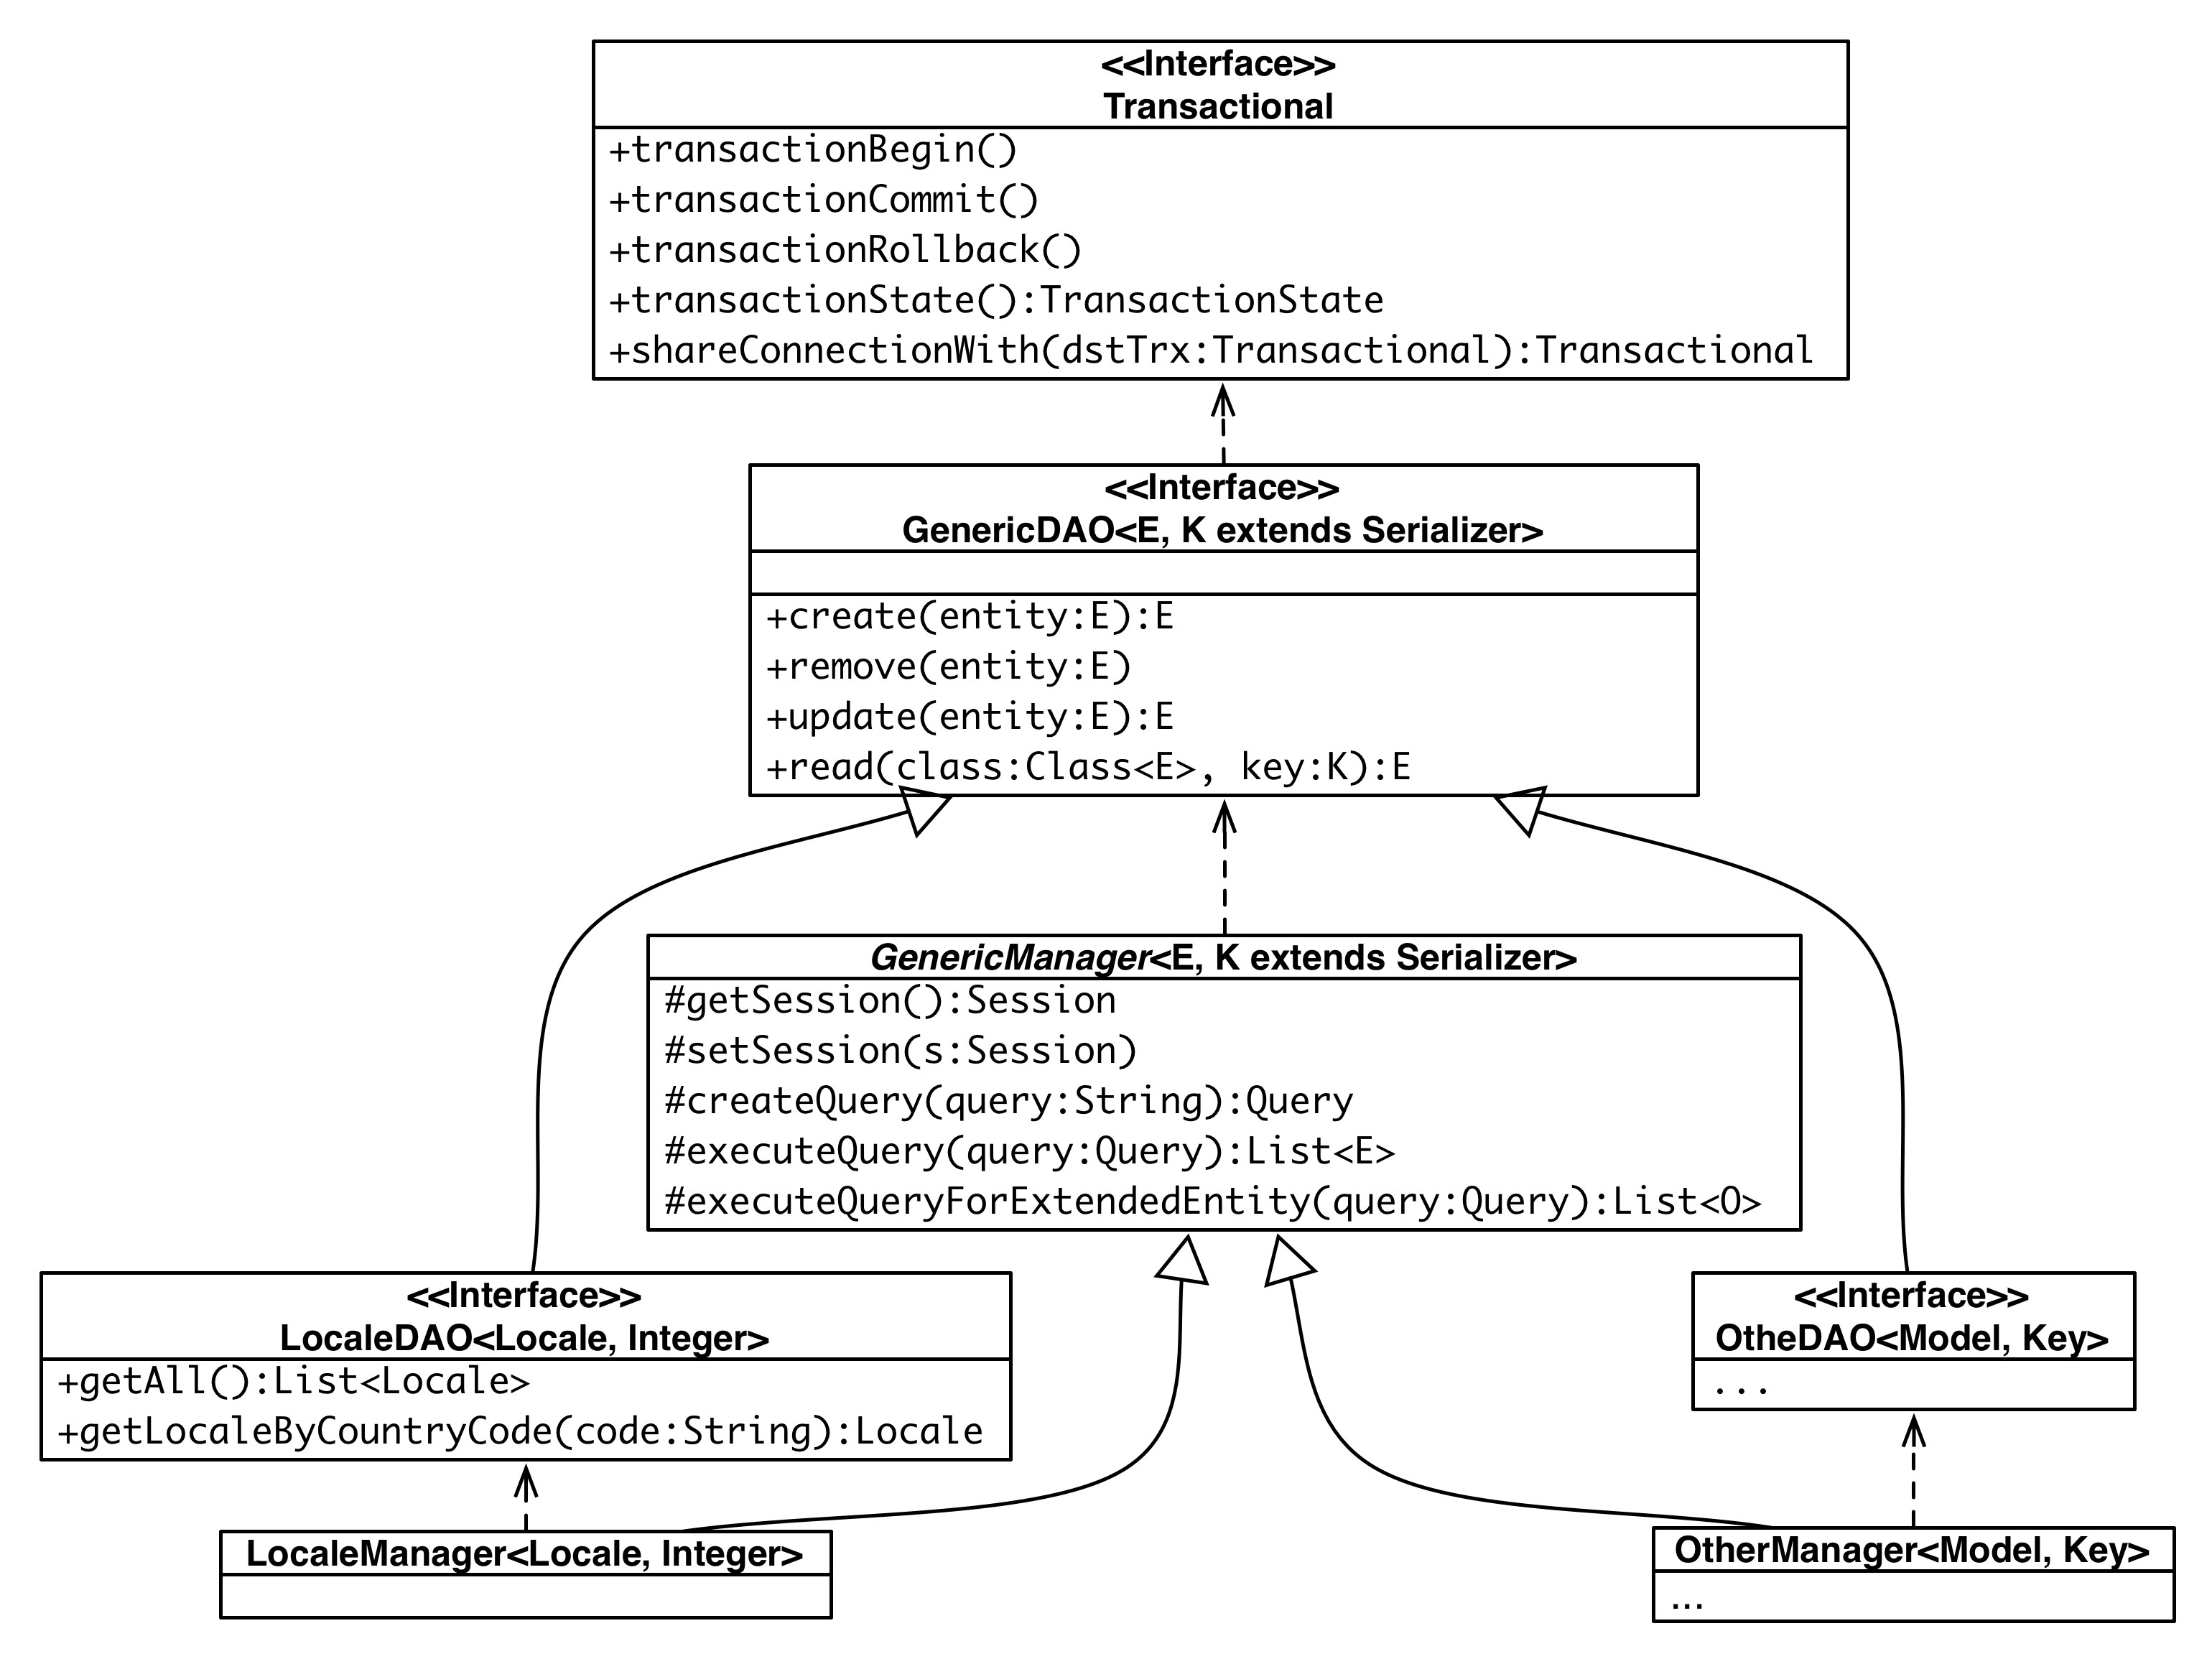
\includegraphics[width=13.2 cm]{./images/umls/uml_diagram_dal.jpg}
   \caption{UML diagram of the DAL core classes.}
   \label{fig:dalUMLDiagrama}
\end{figure}
\\
On top, we have the \verb"Transactional" interface which describes the contract for the manipulation of the transaction. Then the \verb"GenericDAO" describing the CRUD (Create, Read, Update and Delete) operations. The \verb"GenericManager" class implements both interfaces, \verb"Transactional" and \verb"GenericDAO", and it also offers additional helper methods that simplify the implementation of the operations for accessing data.\\
\\
The \verb"GenericDAO" interface and the \verb"GenericManager" class are implemented by each hibernate entity that requires to be accessed within a query. In the concrete \verb"DAO" interface, we describe specific methods that query the database to obtain data and the concrete \verb"Manager" class provides an implementation for those methods as well as for the CRUD operations inherited from the \verb"GenericManager". The specific operations use the~\gls{hql} which is similar to SQL. The Hibernate framework is then responsible for converting the~\gls{hql} into the corresponding SQL code.\\
\\
The service database and log database \gls{dal} uses the structure illustrated in Figure~\ref{fig:dalUMLDiagrama} and both follow the same implementation flow, previously described.
%%%%%%%
%%%%%%%
\subsection{Hibernate Framework Configuration}
\label{subsubsec:hfc}
In this Subsection we describe the configuration aspects of the Hibernate framework along with the additional functionalities that were implemented. We also detail some obstacles that have emerged during the development of the DAL.\\
\\
The Hibernate framework is configured with the \emph{hibernate.cfg.xml} file which contains the information such as the database name, location, user name, password, among others fields. The configuration file also includes information regarding the entity mappings which are defined as a list of references to \gls{hbm} files. The Hibernate tool was installed for the Eclipse IDE, allowing to reverse engineer entities from the database. The auto-generated entity represents the Java object with the associated mapping \gls{hbm} file which describes the attributes and relationship to other entities.\\
\\
Another required configuration of the Hibernate framework is the dialect, which is responsible for generating appropriate SQL for the chosen database. A suitable dialect for our MySQL database is the \verb"MySQL5InnoDBDialect". We had a need to extend it in order to add the mapping for the bitwise operations, since those are not included in the original dialect and cannot be used in \gls{hql}. When the Hibernate framework is initialized, our custom dialect performs registry of the two custom functions (\verb"bitwise_and" and \verb"bitwise_or") that can be used in a \gls{hql} query in order to be correctly converted into corresponding SQL query. The Code Listing~\ref{cod:sqlVShql} shows the usage example for the \gls{hql} with custom defined binary operation which is then mapped to SQL.

\lstset{language=SQL} 
\begin{lstlisting}[frame=single,caption={SQL mapped from HQL.}, label={cod:sqlVShql}, frame=bt]
/* HQL */
SELECT e FROM Entity e WHERE bitwise_and(e.binary1, :someVal) = :someVal
/* SQL */
SELECT e.* FROM entity WHERE e.binary1 & ? = ?
\end{lstlisting}
%%%%%%%
%%%%%%%
\subsection{Difficulties Found in the Implementation}
\label{subsubsec:odi}
Some difficulties were found during the implementation of the DAL, more specifically on the data mapping of the \verb"Localized_Location" table. The first approach consisted in making the field \verb"locale_id" as part of the composite~\gls{pk} and also as the~\gls{fk} for the \verb"city" and \verb"attraction" tables. The~\gls{er} model was valid and successfully generated, but during the creation of the new \verb"Localized_Location" record through the Hibernate framework, the \gls{fk} relationship for the \verb"city" and \verb"attraction" were not included in the generated SQL INSERT statement. This behaviour caused the insertion statement to fail, since \verb"attraction_id" and \verb"city_id" could not be \verb"null".\\
\\
A suitable solution was found for this problem, which consisted in replicating the \verb"locale_id" attribute. The following set of fields were created \{\verb"location_locale_id", \verb"city_locale_id", \verb"attraction_locale_id"\} to replace the original \verb"locale_id".
The implementation of the~\gls{dal} guaranties that has the three fields have always the same value for the specific record.\\
\\
Another problem has emerged when it became necessary to specify different databases in the configuration file. When the hibernate models are generated using the Hibernate Reverse Engineering tool, one of the attributes in the created files is the \emph{catalog} which points to the database used during the code generation process. This binds the model to that database, which is not what we need. However, when the \emph{catalog} attribute is not indicated, the hibernate engine automatically uses the database defined in the configuration file.\\
\\
To circumvent this binding problem, the solution consisted in the creating the Ant~\cite{antTask} task that removes the \emph{catalog} attribute, for each hibernate model file. After generating the hibernate model, it is required to execute the defined Ant task in order to re-process the HBM files.

%%%%%%%%%%%%%%%%%%%%%%%%%%%%%%%%%%%%%%%%%%%%%%%%%%%%%%%%%%%%
\section{REST API}
\label{sec:RestAPIImplementation}
This Section describes different aspects of the implemented \gls{rest}~\gls{api}, and the technologies and methodologies used to design the API.\\
\\
The \gls{rest}~\gls{api} was implemented using the Play Framework. It integrates the components and API required for web application development. The framework is based on a lightweight, stateless, web-friendly architecture that optimizes the resource consumption for scalable applications~\cite{playPerformance}.\\
\\
Our API provides a set of endpoints whose purpose is to obtain data through DAL and serialize the response into \gls{json} format. Every response is composed with header and body. The header contains the information that allows to identify if the request is successfully executed or not. An example of this scenario is illustrated on Code Listing~\ref{cod:guideMeAPIResultEx}. When the header contains the information regarding an error, the body is populated with the null value. The detailed version of the API documentation can be accessed through \verb"Settings/API Documentation" on the Web application.\\
\\
\begin{lstlisting}[language=json,firstnumber=1,caption={Example of the success and error headers.},label={cod:guideMeAPIResultEx}]
/* Success */
{
    "header": {
        "operationSucceeded": true,
        "sessionState": "SessionStateValid" or "SessionStateNotRequired"
    },
    "body": ...
}

/* On error */
{
    "header": {
        "errorMessage": "Length of the locale identifier argument should be exactly 2",
        "operationSucceeded": false,
        "validArguments": false,
        "sessionState": "SessionStateInvalid",
        "friendlyErrorMessage": "Error communicating with the server. Please try again later."
    },
    "body": null
}
\end{lstlisting}
%%%%%%%
%%%%%%%
\subsection{Internationalization Support}
\label{sec:apiInternationalization}
Internationalization is the technique for organizing localized resources so that an application can select the user-preferred set of resources at runtime. Localization is the translation of text displayed by an application. The importance of supporting multiple languages consists in reaching the maximum number of users, specifically in tourist guide applications where users of the application are from different countries. Currently, the API supports English and Portuguese languages, and it is possible to add other languages.\\
\\
Every endpoint receives the \verb"localeName" argument which should have the ISO 639-1 format and sends the response in the corresponding language. The English language is assumed by default when the \verb"localeName" argument is not specified or refers to the unsupported language.\\
\\
When an error occurs during the request, some properties of the header information are populated with the localized information regarding the error in cause, namely the \emph{errorMessage} and \emph{friendlyErrorMessage} properties. These messages are defined as a property list in the \verb"conf/messages.pt" and \verb"conf/messages.en" files. The Play framework offers an easy way to access the localized i18n~\cite{i18nOrigin} properties, as it is shown in Code Listing~\ref{cod:i18nDefinAndUse}.
\newpage
\begin{lstlisting}[language=java,caption={An example of the i18n definition and usage.},label={cod:i18nDefinAndUse}, frame=bt]
Message.UserName=Nome Completo    # messages.pt
Message.UserName=Full Name        # messages.en
------------------------------
// Depending on the current language, the framework will obtain 
// the localized value for the  Message.UserName key
String example = Messages.get("Message.UserName") + ":" + user.getName();
\end{lstlisting}
%%%%%%%
%%%%%%%
\subsection{Implementation Details}
\label{sec:apiImplementation}
A flexible structure was developed to generalize and facilitate the implementation of every endpoint action. The~\gls{uml} diagram shown on Figure~\ref{fig:umlAPICore} illustrates the core classes involved in the operation. The \verb"WebOperationResponse" class represents the response of the operation and it contains the header and body information.
\begin{figure}[h!]
 \centering
   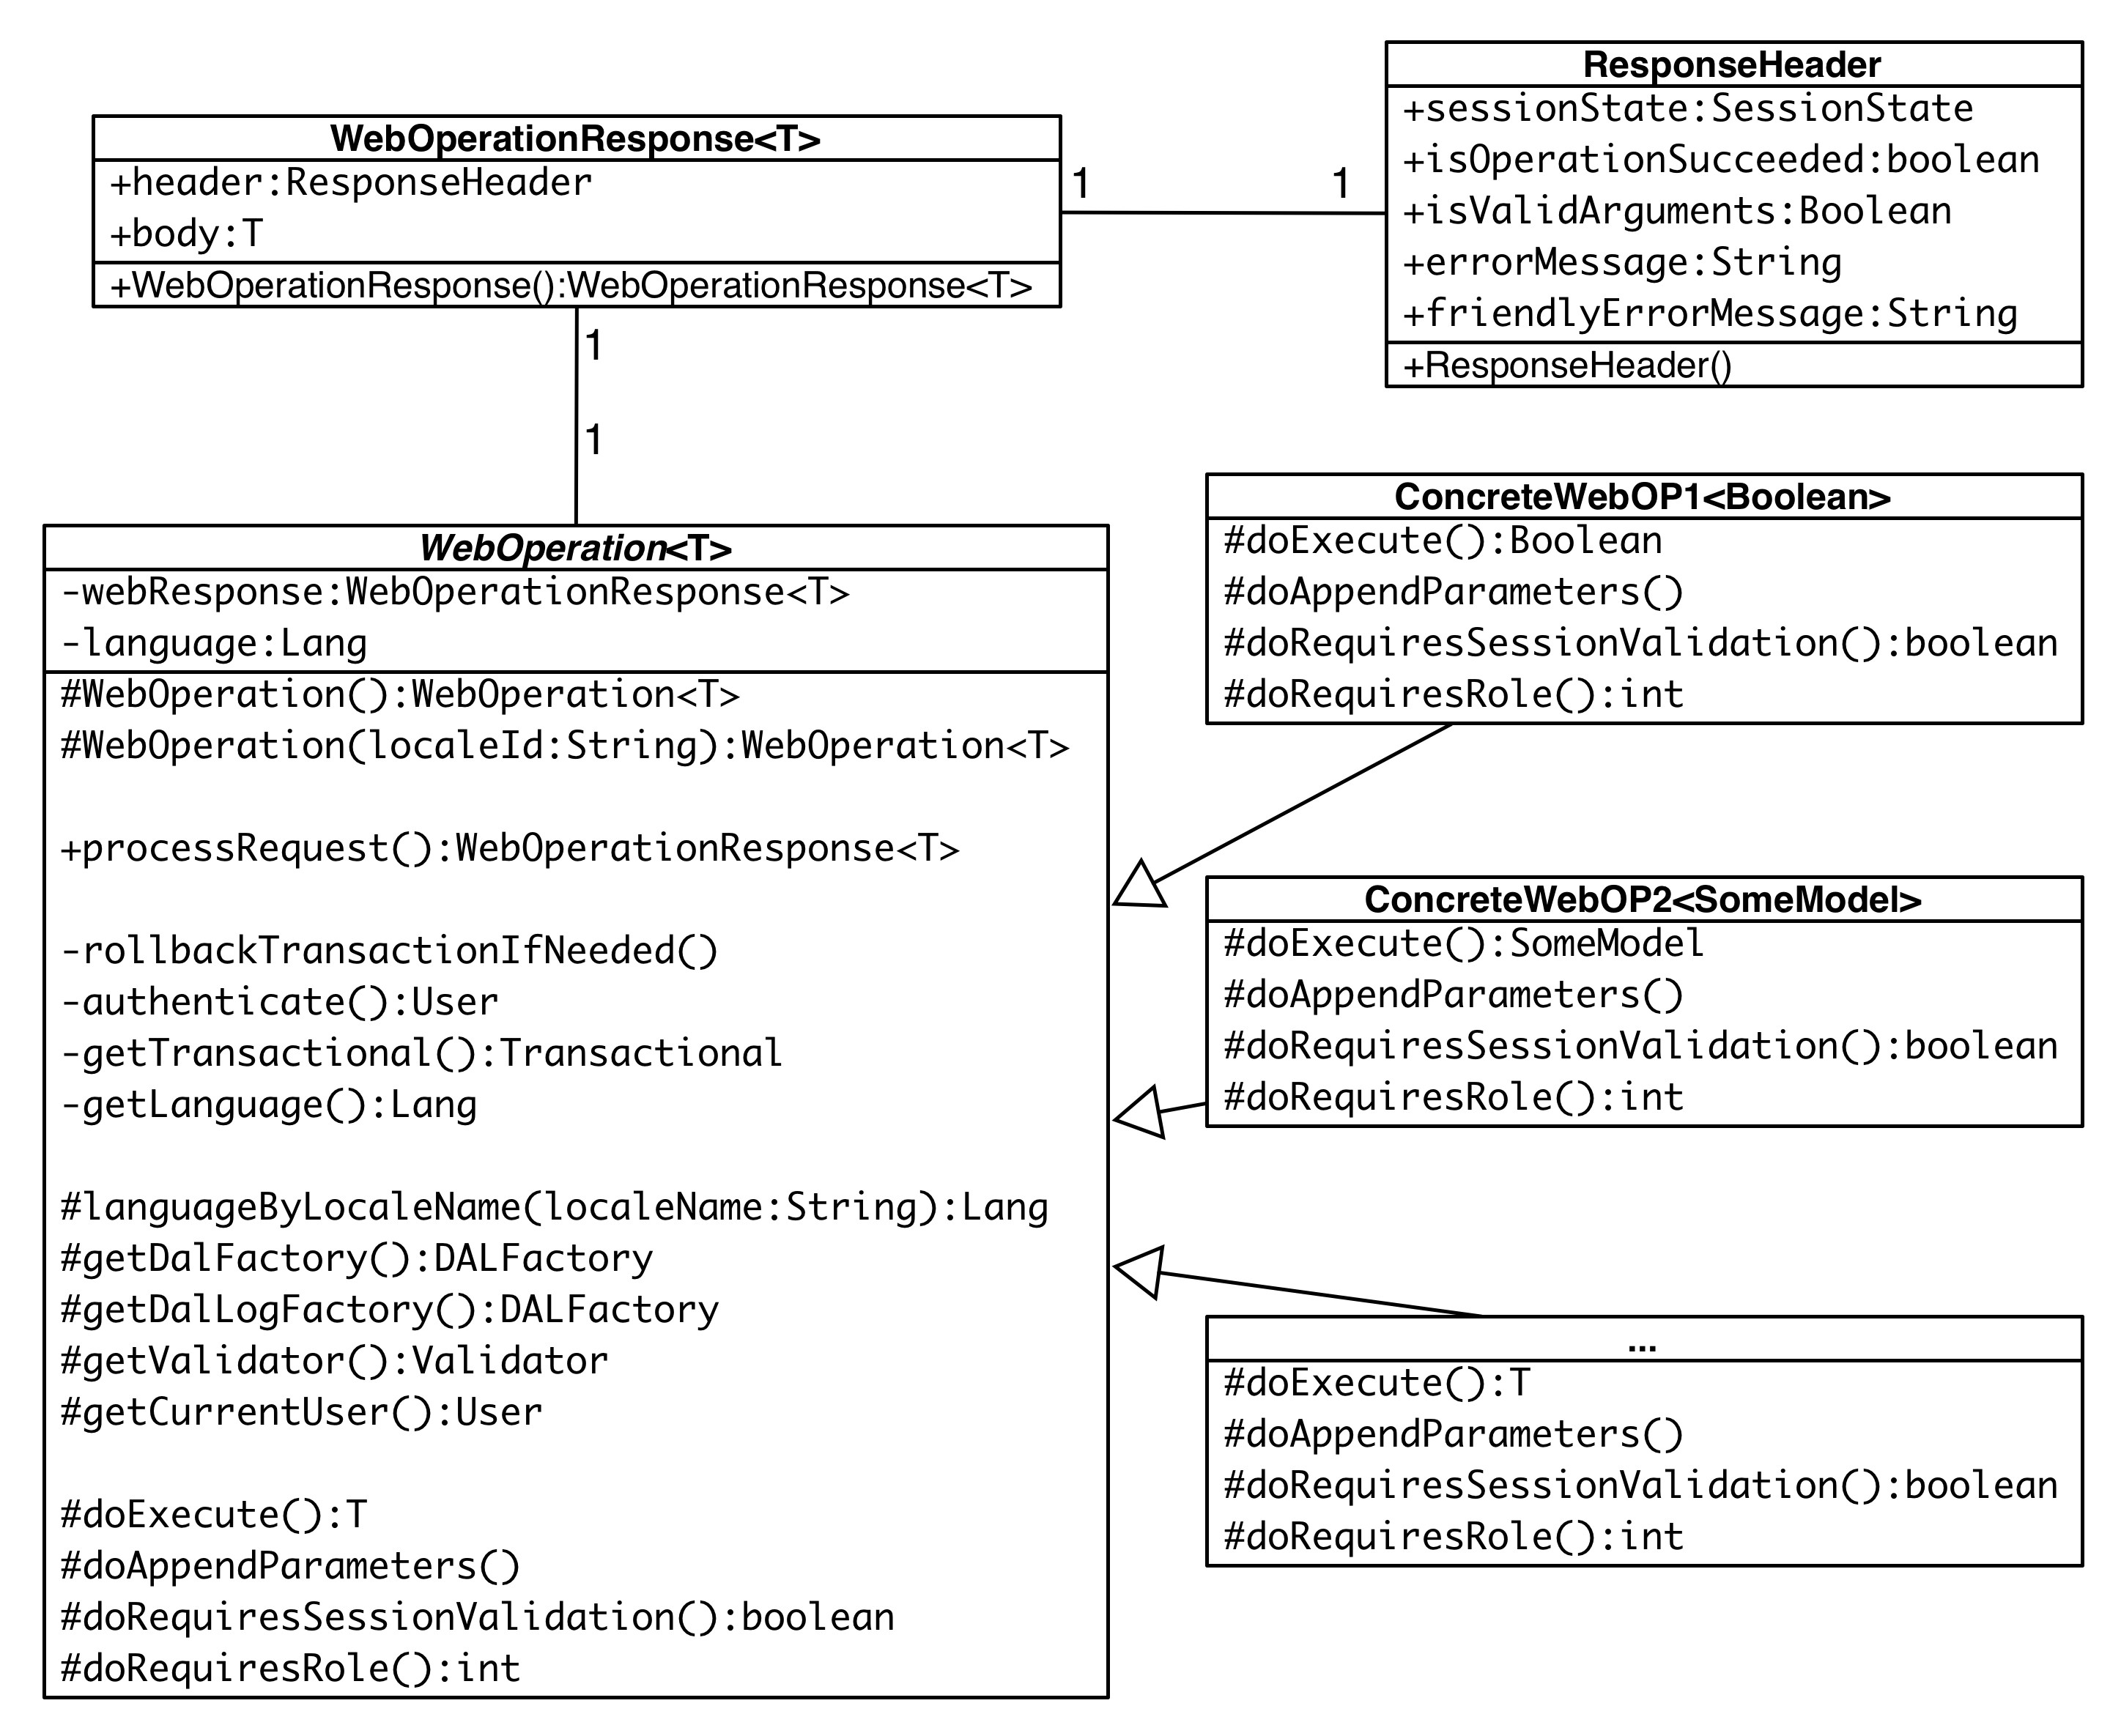
\includegraphics[width=13cm]{./images/umls/uml_diagram_api_core.jpg}
   \caption{UML diagram representing the core structure of the API.}
   \label{fig:umlAPICore}
\end{figure}
\\
The processing flow of the web operation is shown in Figure~\ref{fig:webOperationFlow}, which describes the actions taken by the  \verb"processRequest()" method:
\begin{figure}[h!]
 \centering
   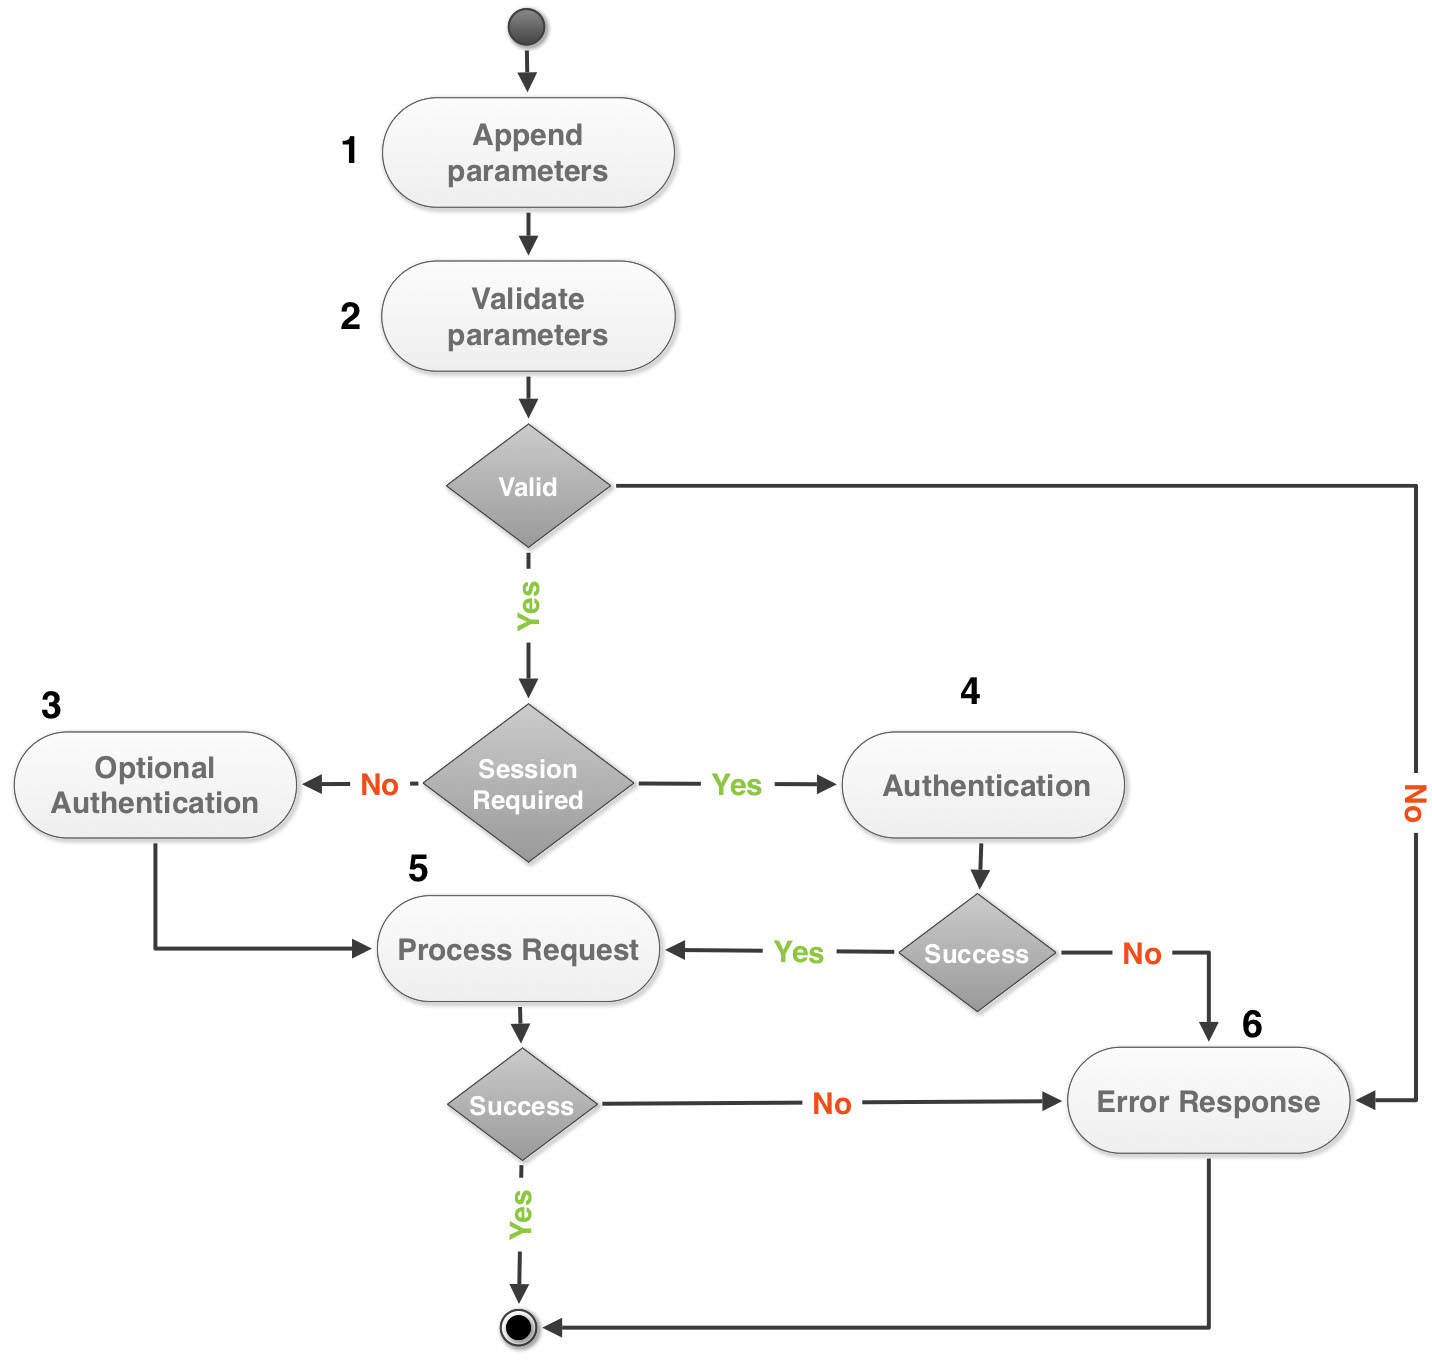
\includegraphics[width=9cm]{./images/flows/flow_web_operation_flow.jpg}
   \caption{Operation's validation and processing.}
   \label{fig:webOperationFlow}
\end{figure}
\begin{enumerate}
\item Concrete operation class adds the parameters to the validator.
\item Every parameter is validated to ensure that it is within the defined restrictions. If any of the parameters is invalid, the response header will contain the information explaining the error cause.
\item When the user authentication is optional, we verify if the sessionToken is passed, and if so, we fetch the user's information through the DAL. Any error that occurs during this phase is ignored. 
\item When user authentication is required, same actions are performed to retrieve the user information, but if any of these actions fails, the error response is generated.
\item The \verb"doExecute()" method from the child class is invoked, which is responsible for obtaining and processing the body of the response. If the operation succeeds, the response is populated with the result, otherwise it contains the information regarding the error content.
\end{enumerate}
If some unexpected error occurs during the \verb"processRequest()", through the DAL, its cause is registered to the log database for later analysis.\\
\\
Each web operation is implemented as a separate class which inherits the \verb"WebOperation<T>" where \verb"T" represents the type of the response upon the success. Every action delegates all the processing and validation to the respective instance of the \verb"WebOperation" and its endpoints path are in the \verb"conf/routes" configuration file. This file lists all the routes implemented by the API. Each route consists of an HTTP method and \gls{uri} pattern which are associated to an action method. The single route definition example is shown in Code Listing~\ref{cod:routeFile}.
\newpage
\begin{lstlisting}[language=java,caption={An example of the route file entry.},label={cod:routeFile}, frame=bt]
GET  /user/authenticate  controllers.User.authenticate(loc:String,tkn:String)
\end{lstlisting}
The responses of the web operation are serialised in \gls{json} format. When sent to user, the HTTP Header representing the \verb"content-type" is populated with \verb"application/json" value. The serialisation is achieved by using the  \gls{json} Jackson~\cite{jsonJackson} processor. During the development of the API we configured this framework to not serialize the attributes of the response when those are populated with \verb"null". The most direct example is the \verb"ResponseHeader", which excludes attributes presented in Code Listing~\ref{cod:optionalyProperties} when the response is successfully executed. Entities that represent information regarding the \verb"Location" and \verb"User" were also configured in the same manner.
\begin{lstlisting}[language=java,caption={Optional properties of the ResponseHeader.},label={cod:optionalyProperties}, frame=bt]
"errorMessage": null,
"validArguments": null,
"friendlyErrorMessage": null
\end{lstlisting}
This configuration allows to minimise the bandwidth occupied during the transmission of the response. With the illustrated example, we have spared 73 bytes, because that information would not be sent as part of the response, which equals to 1Mb for approximately each 15000 requests. For a large API usage, it will significantly minimise the amount of information to be sent from the server where the API is hosted and may increase the response time.
%%%%%%%
%%%%%%%
\subsection{Authentication}
\label{subsec:authentication}
Most of the implemented web operations retrieve data from the database through the DAL. But, the operations related to the authentication are different, since users can authenticate themselves on the service by using their Facebook~\cite{facebook} or Twitter~\cite{twitter} accounts. If the user exists, a session token is generated, allowing to execute API operations that require authentication. When the user authenticates himself by the first time, the service automatically creates a new account for that user. For the Facebook authentication, we use RestFB~\cite{restfb} framework that allows to obtain information regarding the users such as, name, email, among others fields. Then, the information is mapped directly to the Java classes. The framework provides an easy way to navigate through the Facebook Graph API~\cite{facebookGraphAPI}.\\
\\
Twitter's authentication service is managed in a similar way. To interact with the Twitter REST API v1.1~\cite{twitterRestAPI} we have used Twitter4j~\cite{twitter4j} library which already handles the authentication and provides wrappers to access user's information.\\
\\
Both services implement the authentication using the OAuth 2.0~\cite{oauth2} protocol. From the application side, the user should perform authorization using the preferred service. Then, the authorization data (token, token secret, and expiry date) is sent to our authorization endpoint and used to obtain information regarding the user in question. Finally, this information is used to populate the database with user's information and consequently perform the authentication.
%%%%%%%
%%%%%%%
\subsection{Location Creation}
\label{subsec:locationCreation}
During the location creation, users have to pick the location positioning coordinates from the map. When those are submitted to the service, the information regarding the location such as city, country, and address, are obtained automatically through the Reverse Geocoding~\cite{googleGeocodingAPI} process. The~\gls{gg}~\gls{api} is used for this purpose by allowing to extract human-readable address from a map location.\\
\\
The descriptive information regarding the address can be obtained in different languages. As of the time of this writing, the latest API version (v3) supports 55 different languages and dialects~\cite{googleGeocodingLanguages}. An example of a GG request (asking information about localization with latitude=38.76347 and longitude=-9.093783) is presented below:\\
\\
\verb"http://maps.googleapis.com/maps/api/geocode/json?latlng=38.763470,-9.093783&"\\
\verb"sensor=false&language=pt"\\
\\
Code Listing~\ref{cod:GoogleReverseGeocoddingJSON} shows an example of the~\gls{gg} response for the request presented above.
\begin{lstlisting}[language=json,firstnumber=1,caption={Google Geocoding JSON response example.},label={cod:GoogleReverseGeocoddingJSON}]
{
 "results" : [ {
     "address_components" : [
       {
         "long_name" : "Lisboa",
         "short_name" : "Lisboa",
         "types" : [ "locality", "political" ]
       },
       {
         "long_name" : "Portugal",
         "short_name" : "PT",
         "types" : [ "country", "political" ]
       },
       {...}
     ],
     "formatted_address" : "Passeio Ulisses 9, 2715-311 Lisboa, Portugal",
   },
   ...],
 "status" : "OK"
}
\end{lstlisting}
The \verb"language" attribute is the union of the ISO 639-1 and RFC 3066~\cite{rfc3066} standards, so its value is adapted according to the system language, which follows the ISO 639-1 format.
%%%%%%
%%%%%%
\subsection{Location Filtering}
\label{subsec:locationFiltering}
The REST API provides a set of methods that allow to perform different operations, such as authentication, lookup for points of interest, among others. There is a specific set of endpoints to perform the filtering of the touristic locations. Operations that obtain visited, recommended, and wanted locations are not subject to filtering criteria.\\
\\
Touristic location filtering can be achieved with \verb"/location/filter" endpoint where most of the arguments are optional. It allows to specify any combination of the arguments, easily adapting to user needs. It is possible to have any permutation of the filtering criteria such as city name, attraction, weather conditions, distance, among others.\\
\\
When the geographic coordinates pointing to user's current location are retrieved from the device, the latitude and longitude are passed to the service during the queries related to location filtering. We use this information to compute the distance between the user and location, presenting the results sorted increasingly by distance. For this purpose, we have used the Spherical Law of Cosines~\cite{sphericalCosine}, with the following set of equations:\\
\begin{equation}
  \begin{aligned}
    &\phi_{1} = userLat \times \frac{\pi}{180} \\
	&\phi_{2} = locationLat \times \frac{\pi}{180} \\
	&\Delta_\lambda = (userLon - locationLon) \times \frac{\pi}{180} \\
	&R\bigotimes = 6371\\
	\\
	&d = acos( sin(\phi_{1}) \times sin(\phi_{2}) + cos(\phi_{1}) \times cos(\phi_{2}) \times cos(\Delta_\lambda) ) \times R\bigotimes
  \end{aligned}
\end{equation}
where the $\phi_{1}$ represents user's latitude, $\phi_{2}$ refers to the location's latitude, and the $\Delta_\lambda$ is the difference between the user's and location's longitude coordinate. These values are converted to radians. The $R\bigotimes$ is a constant representing the distance in kilometres from Earth's center to its surface. The result $d$ represents the distance in kilometres between the user's specified coordinates and the touristic location at hand.

%%%%%%
%%%%%%
\subsection{Integration with World Weather Online}
\label{subsec:integrationWWO}
Users can preview the temperature when they are consulting the details of the chosen touristic location. For this purpose, we have made integration with the World Weather Online (WWO)~\cite{wwo} public API which allows to access current weather conditions. Their API allows to consult detailed information regarding the weather and supports different response formats, namely the~\gls{xml}, \gls{csv}, and JSON. We are only consulting the information regarding the weather condition and temperature, with the response being serialized into JSON format.\\
\\
The main reasons for choosing this service is that it doesn't require any commercial license, it can be used for personal and commercial purposes, and provides reliable information regarding current weather. The free version of this API is limited to 500 requests per hour.\\
\\
The weather conditions and the temperature are obtained using the geographic coordinates of the location in cause. When the information is successfully obtained, it is stored into the database and considered valid for the next 3 hours. This implies that subsequent requests for the location details will not trigger any call to the \gls{wwo} API, improving significantly the response time of our service and still provide the user with the updated and accurate weather information.\\
\\
Currently, the \gls{wwo} API supports around 48 different statuses for classifying the weather conditions~\cite{wwoCodes}. For this project, many of these statuses are not relevant, so we have shortened this set into 6 in order to represent the most common weather conditions. After querying the \gls{wwo} service, the weather condition value is converted into our domain specified value and our users are provided with minimalistic information regarding this matter. As an example, the \gls{wwo} API provides more than 15 statuses for classifying the rainy weather condition, when this information is received, it's mapped as \emph{rainy}, thereby minimizing the amount of redundant information. 

%%%%%%%%%%%%%%%%%%%%%%%%%%%%%%%%%%%%%%%%%%%%%%%%%%%%%%%%%%%%
\section{Recommender system}
\label{sec:recommenderService}
The Recommender system is one of the key features of the GuideMe service. In order to provide quality recommendations for our users, we have used the Apache Mahout Recommendation Engine library~\cite{apacheMahout}. Mahout provides a varied set of the Collaborative Filtering algorithms, for user and item based recommendations. Nowadays, this library is widely used for the implementation of recommendation systems.\\
\\
As we have described in Chapter~\ref{theory}, due to recommendation quality and algorithm performance benefits we have chosen the Item-Based Collaborative Filtering approach as our candidate for the recommender system. The implemented recommender system is implemented with the Slope One algorithm and scheduled with the Cron job to run every day at 3:00 AM. The chosen algorithm has proven to be fast, but overall performance has it's drawbacks when the datasource uses information from the database. To improve the performance of the recommendation system, we have imposed some restrictions which consist in selecting the users that should receive new recommendations. Through DAL, the service obtains a list of users who are eligible\footnote{By eligible users, we consider users that have visited at least one location.} for recommendations, and then for each user we apply the following equation:\\
\begin{equation}
PVu = VSR/TV,
\end{equation}
where $PVu$ is the percentage of the visited locations since last recommendation, for specific user $u$. $TV$ represents the total number of visited locations and $VSR$ refers to the number of the visited sights since last recommendation. The new recommendations are only computed if the user had an increase of $5\%$ of the visited locations. This selection allows to improve algorithm performance by excluding users that don't have new visited locations. We consider that the change on the number of visits below $5\%$ is meaningless regarding the recommendation results. Finally, we remove all previous recommendations and populate the database with new results.\\
\\
To accelerate the recommendation process by taking the advantage of the processing power, users eligible for new recommendations are divided into equal sets. Each set is passed to a different thread where the recommendations are computed and stored to the database.

%%%%%%%%%%%%%%%%%%%%%%%%%%%%%%%%%%%%%%%%%%%%%%%%%%%%%%%%%%%%
\section{Mobile Application}
\label{sec:iosApplication}
In this Section we describe the implementation aspects of the iOS mobile application, what kind of operations and features it offers and how those features were implemented. We start by detailing the communication layer between our service and iOS application. Then, we present the application overview, followed by aspects regarding the internationalization.\\
\\
The iOS application is implemented following the concept of universal app. A universal app is a single application that is optimized for iPhone, iPod touch, and iPad devices. The final product is a representation of a single binary that adapts to the current device. When searched on the App Store~\cite{appleAppStore} the same binary is shown for the iPhone/iPod and iPad devices instead of having different binaries for each device.\\
\\
The development of the universal binary involved extra work. Because of the differences in device screen sizes, most of windows, views, and view controllers code for iPad is different from the code for iPhone and iPod touch. In addition, there are some differences between interface principles in iPhone and iPad platforms, which are described along in iOS Human Interface Guidelines~\cite{appleiOSGuideLines}.\\
\\
Users usually prefer an universal app instead of a device-specific. They need to download it only once, and if an app is correctly designed, every additional feature that they activate is automatically enabled across all devices using the iCloud~\cite{appleiCloud} service.
%%%%%%%
%%%%%%%
\subsection{Communication Layer}
\label{subsec:iosCommunicationLayer}
A flexible interface for the communication with the service was designed to facilitate the developments of the iOS applications. Figure~\ref{fig:umliOSServiceLayer} shows the~\gls{uml} diagram describing the main classes responsible for the communication with the service infrastructure. Every concrete implementation of the model inherits the \verb"BaseModel" and implements the \verb"parserWithJson" method from the \verb"ParserProtocol". This method ensures that the model knows how to parse properties from the response serialized in \gls{json} format.
\begin{figure}[h!]
 \centering
   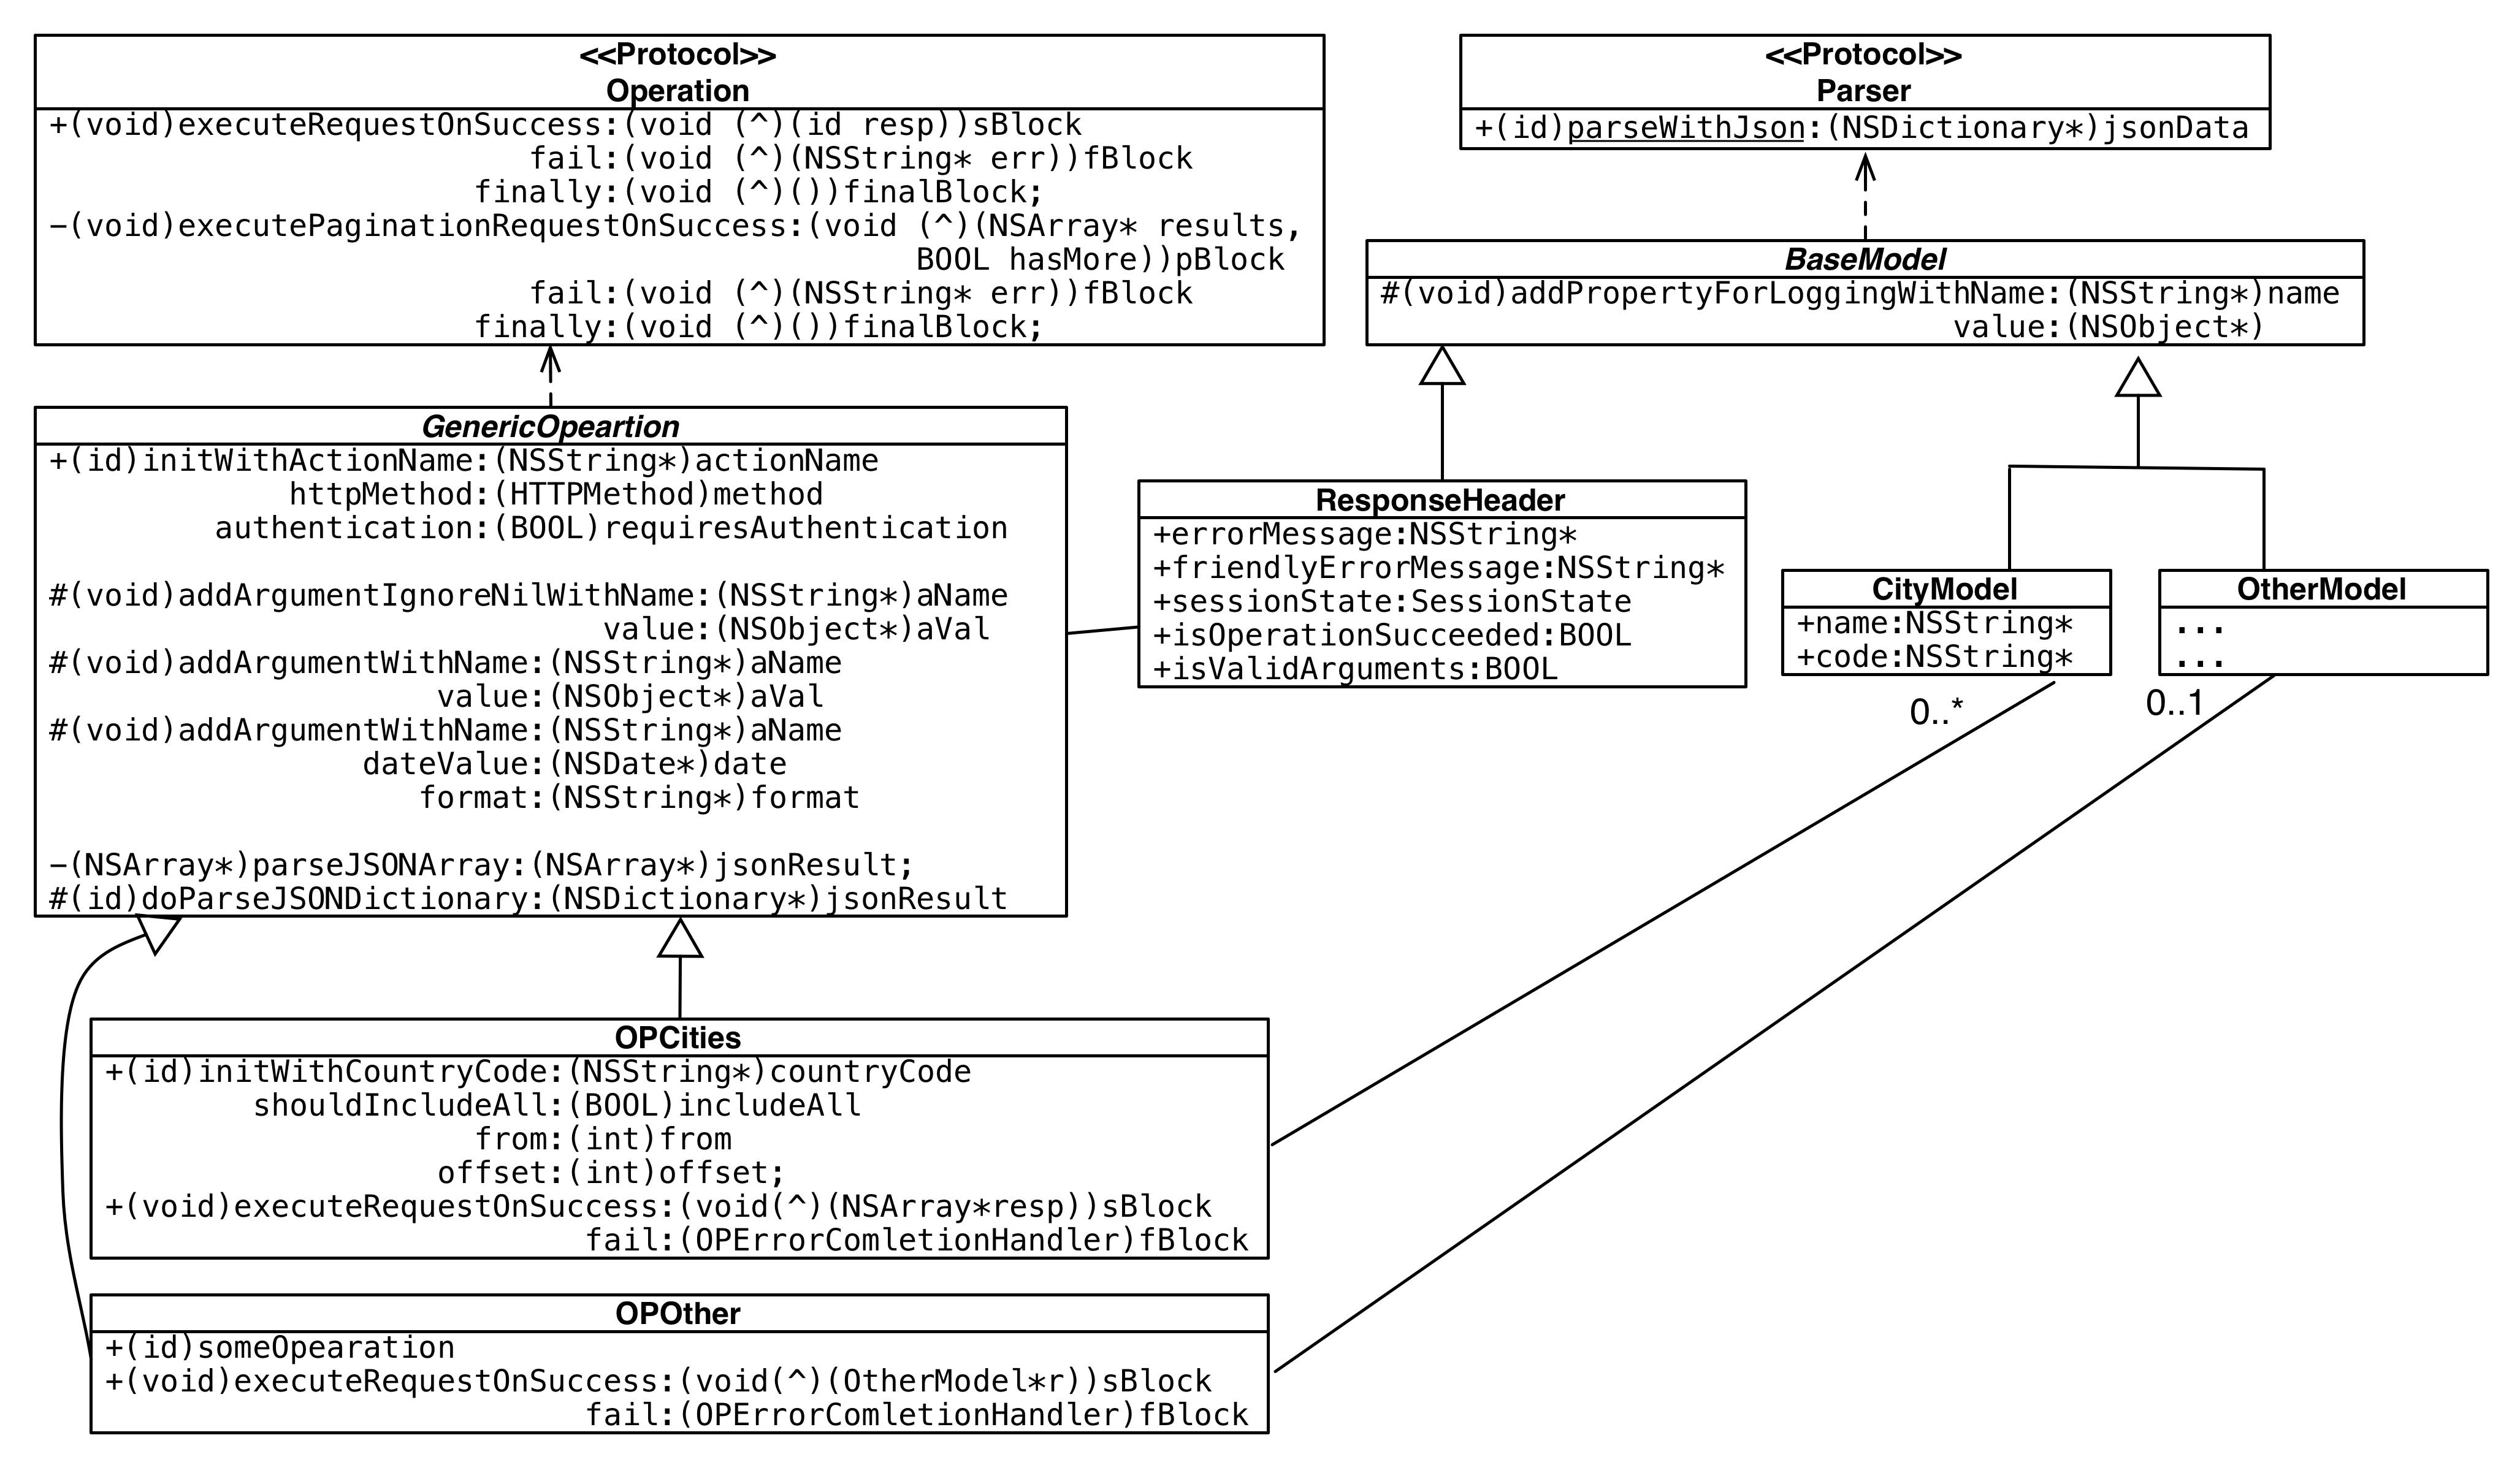
\includegraphics[width=11.8cm]{./images/umls/uml_diagram_ios.jpg}
   \caption{UML diagram representing the communication layer of the iOS application.}
   \label{fig:umliOSServiceLayer}
\end{figure}
\\
The \verb"GenericOperation" class is responsible for making the request to the endpoint defined by the child class. The request is executed as a background task using the~\gls{gcd}\footnote{\gls{gcd} comprises language features, runtime libraries, and system enhancements that provide systemic, comprehensive improvements to the support for concurrent code execution on multicore hardware in iOS and OS X~\cite{gcd}.}, which allows to execute the request asynchronously in a background thread. Figure~\ref{fig:iosExecutionFlow} illustrates the most important steps required to perform the remote request, which are detailed as follows:\\
\begin{enumerate}
\item The class that inherits the \verb"GenericOperation" specifies the endpoint and the HTTP method required to perform the operation.
\item The parameters are appended to the request.
\item The remote request is performed on a background thread.
\item When the response arrives, it is validated and parsed.
\item The failure block is invoked on the main thread when the response is invalid or the header is populated with information regarding an error.
\item The success block is called on the main thread if everything goes as expected.
\item If the user has specified the finally block, it will be executed on the main thread after the success or failure blocks.
\end{enumerate}
\begin{figure}[h!]
 \centering
   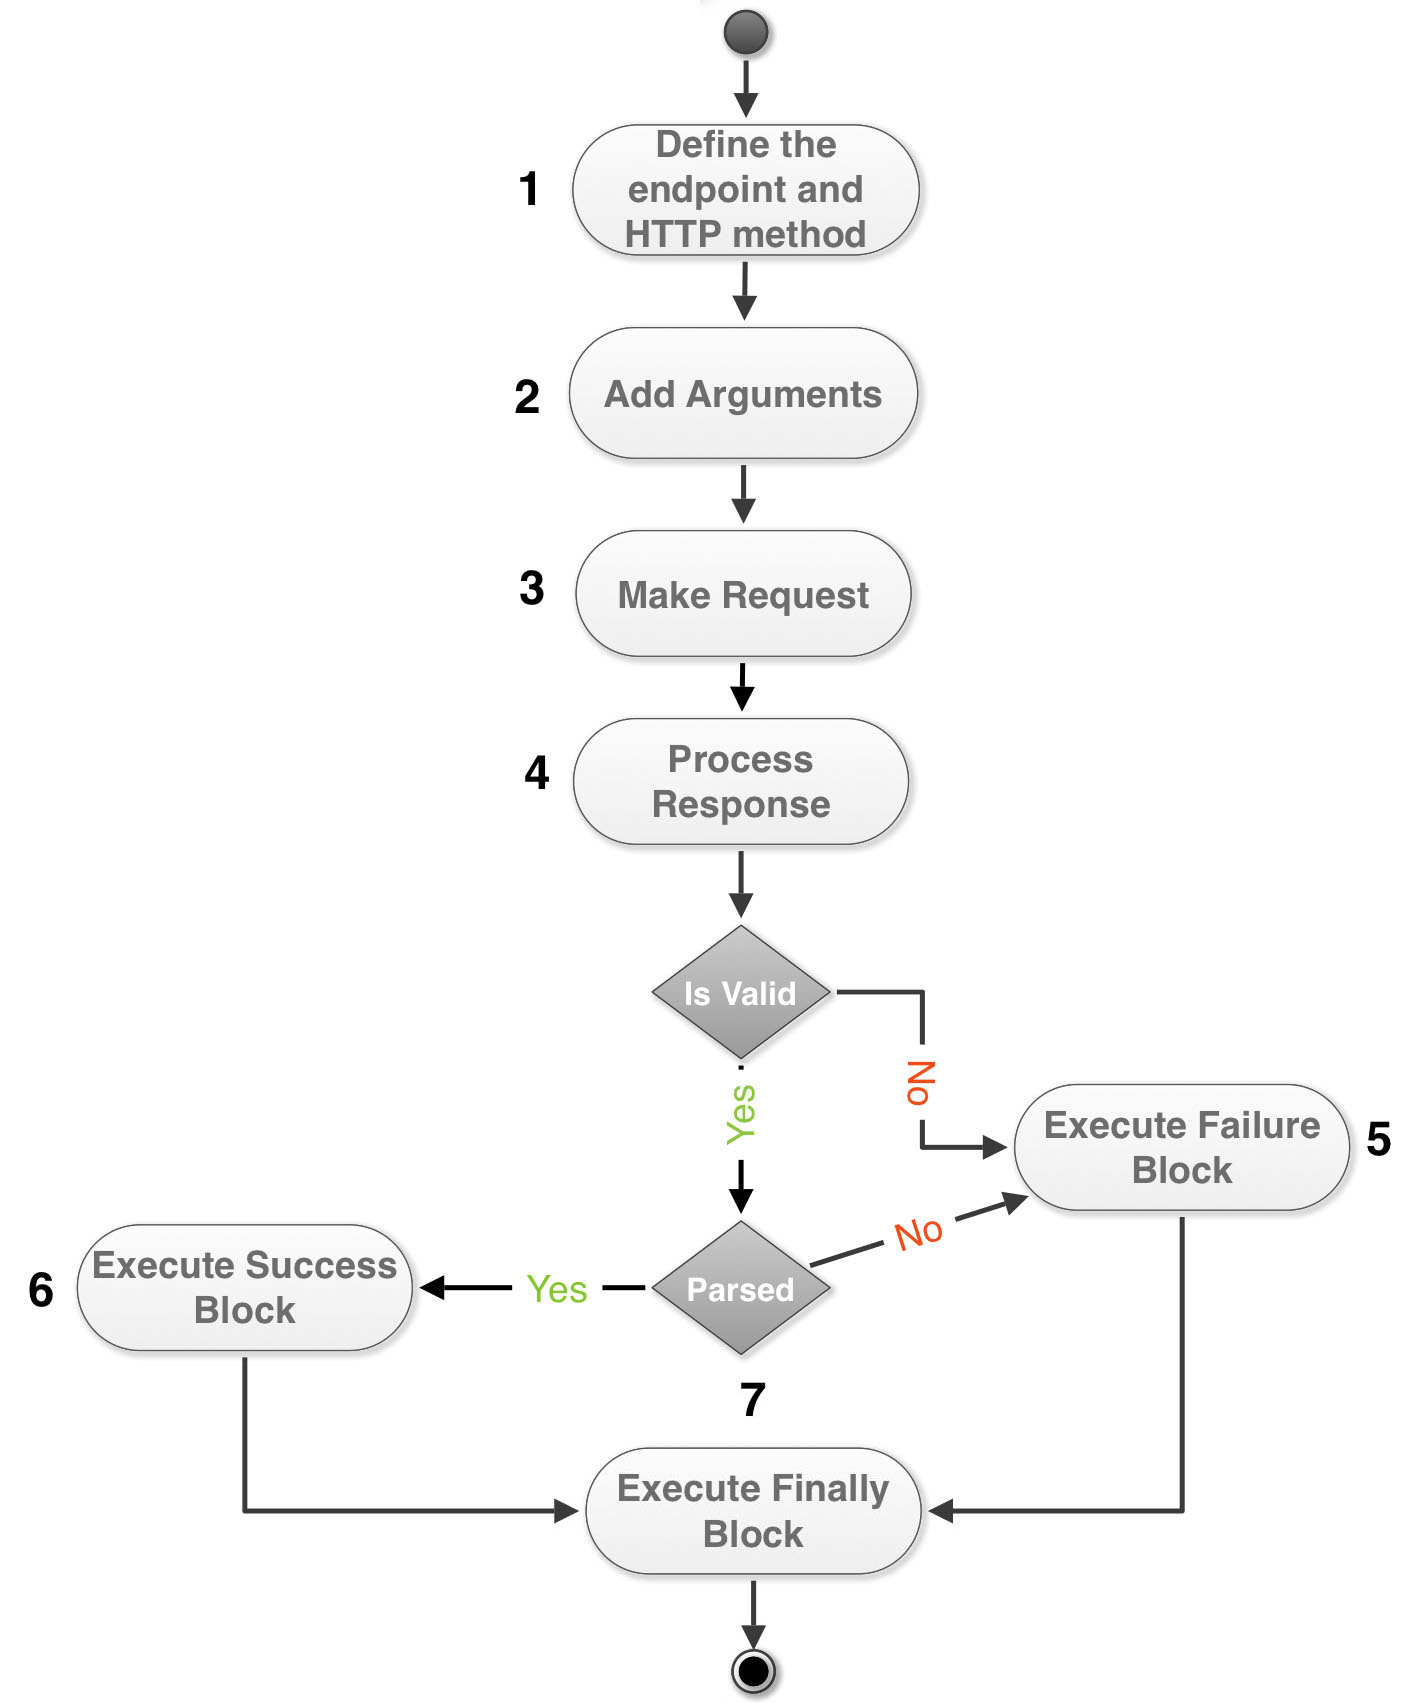
\includegraphics[width=9cm]{./images/flows/flow_ios_operation_flow.jpg}
   \caption{Processing of the remote request.}
   \label{fig:iosExecutionFlow}
\end{figure}
The implementation with blocks has simplified the usage of the classes that perform the remote requests. The current approach performs the background task to handle the request and invokes the described blocks on a main thread, allowing to implement the \gls{ui} operations directly inside the respective block. As a consequence, we minimise the amount of code to be written. Code Listing~\ref{cod:iosGCDCommonApproach} illustrates an example of the common implementation to perform such tasks in a background thread and then update the \gls{ui} on the main thread.\\
\begin{lstlisting}[language={[Objective]C},caption={An example of the remote request using common GCD approach.},label={cod:iosGCDCommonApproach}, belowskip=3em, frame=bt, ]
dispatch_queue_t getCitiesQueue = dispatch_queue_create("get cities", NULL);
   dispatch_async(getCitiesQueue, ^(){
      NSError ** error;
      NSArray * cities = [CitiesOP performOperationWithCountryCode:@"PT" 
                          shouldIncludeAll:NO from:0 count:10 error:&error];
      dispatch_async(dispatch_get_main_queue(), ^(){
         if(!cities){ /* Notify user about the error */ }
         else{        /* Handle the "cities" response here */ }
         // Perform some common operations
         });
});
\end{lstlisting}
The adopted solution, shown in Code Listing~\ref{cod:iosGCDImproovedApproach} simplifies the readability and amount of code to be written. The scheduling to the background thread and the main thread are made internally by the implemented infrastructure.\\
\begin{lstlisting}[language={[Objective]C},caption={An example of the remote request using the adopted solution.},label={cod:iosGCDImproovedApproach}, frame=bt]
OPCities *citiesOP = [[OPCities alloc] initWithCountryCode:@"PT" 
                                          shouldIncludeAll:NO 
                                                      from:0 
                                                     count:100];
[citiesOP executeRequestOnSuccess:^(NSArray *cities){
   // Handle the "cities" response here
 } fail:^(NSString *errorMessage){
   // Notify the user about the occurred error
 } finally:^(){
   // Implementation of some common actions
}];
\end{lstlisting} 
%%%%%%%
%%%%%%%
\subsection{iOS Application Overview}
\label{subsec:ioHighlightedFeatures}
The developed mobile application offers two interfaces. The common interface which can be accessed by any user and the interface for administration.
All users can consult points of interest near their current location, apply filtering criteria (e.g. filtering by country, city, category, weather conditions, among others) to shorten the amount of results. Users also have the possibility to consult recommended locations, mark locations as visited or wanted, follow and unfollow other users.\\
\\
Users with the administrative privileges have access to all of the described tasks. They can also insert new or update an existing touristic location, and consult information regarding the reported touristic locations. The main focus of the mobile applications is the users's current location, which is represented by the geographic coordinates obtained using the positioning service available on the user's device, such as~\gls{gps} or Wi-Fi. By knowing the users's current location, the service can compute the distance between the touristic location and the user's location, as discussed before (Subsection~\ref{subsec:locationFiltering}). When the location services are not available, the service continues to allow consulting of the points of interest but without the indication of the distance between the user and the touristic location at hand.\\
\\
Figure~\ref{fig:guideMeWebScreenshotsIOSFull} illustrates some of the implemented features of the application for iPhone.
\begin{figure}[h!]
\begin{center}
		\centering
        \begin{subfigure}[b]{0.30\textwidth}
	     		\centering
                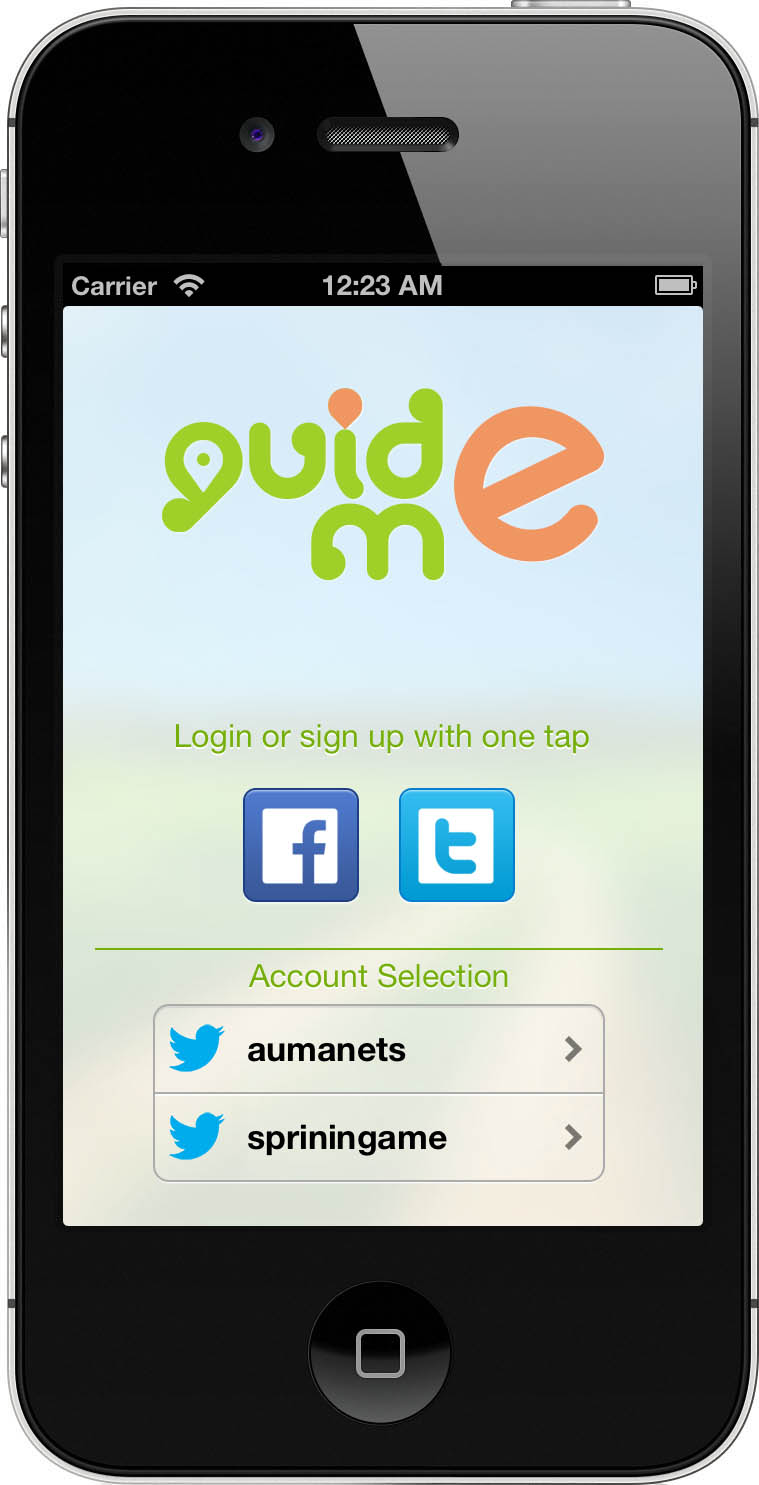
\includegraphics[height=8cm]{./images/screenshots/screenshot_iphone_app_1.jpg}
                \caption{Login screen.}
                \label{fig:guidemeWebScreenshotsIOSFina1}
        \end{subfigure}%
        \begin{subfigure}[b]{0.30\textwidth}
 				\centering
                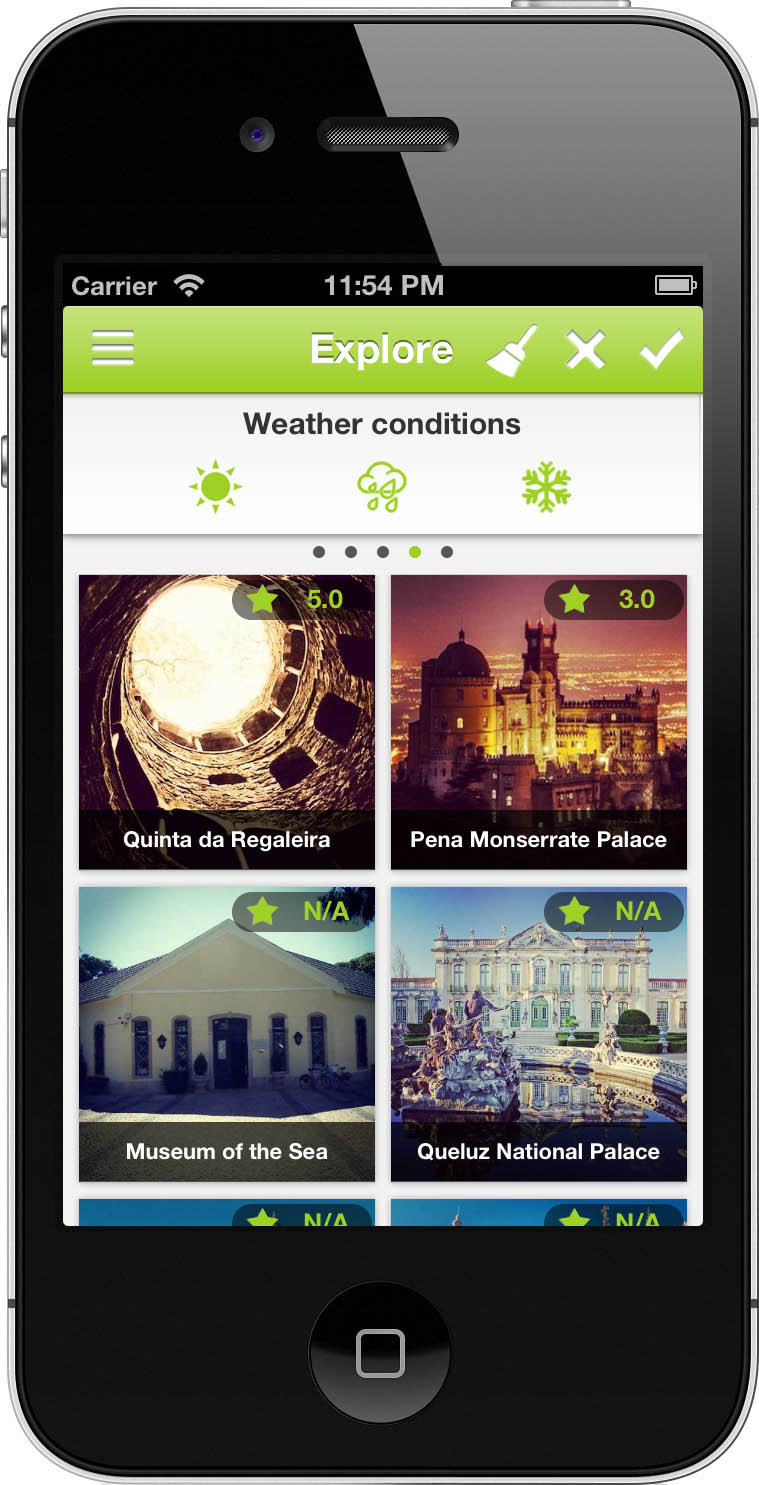
\includegraphics[height=8cm]{./images/screenshots/screenshot_iphone_app_2.jpg}
                \caption{Location search.}
                \label{fig:guidemeWebScreenshotsIOSFina2}
        \end{subfigure}
        \begin{subfigure}[b]{0.30\textwidth}
 				\centering
                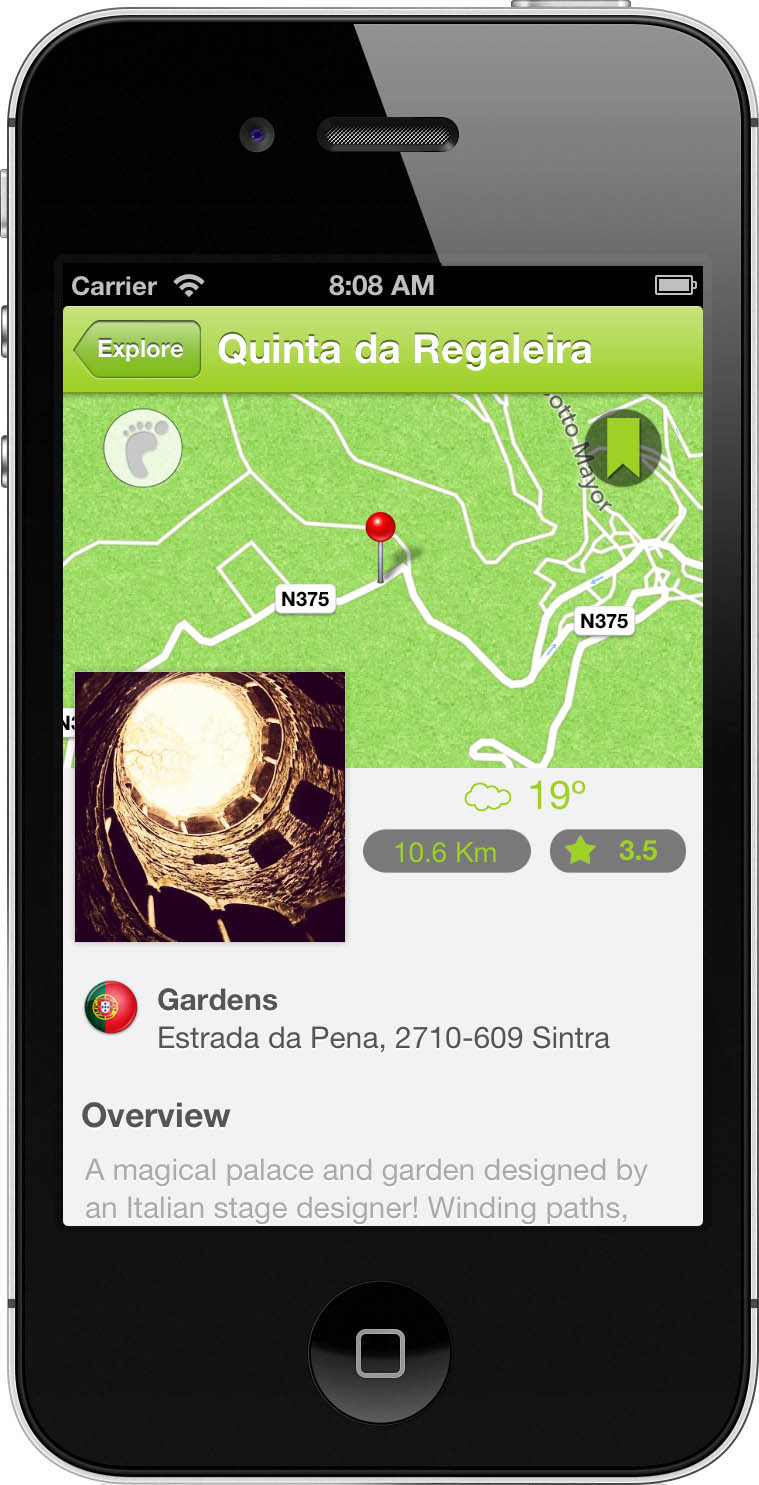
\includegraphics[height=8cm]{./images/screenshots/screenshot_iphone_app_3.jpg}
                \caption{Location details.}
                \label{fig:guidemeWebScreenshotsIOSFina3}
        \end{subfigure}
        \caption{Screenshots of the iPhone application}
        \label{fig:guideMeWebScreenshotsIOSFull}
        \end{center}
\end{figure}
In Figure~\ref{fig:guideMeWebScreenshotsIOSFull}~(\subref{fig:guidemeWebScreenshotsIOSFina1}) we have the login screen, where the user may choose the preferred social service in order to perform login or sign up. Figure~\ref{fig:guideMeWebScreenshotsIOSFull}~(\subref{fig:guidemeWebScreenshotsIOSFina2}) shows a list of the locations, which have resulted from the applied filtering criteria. The detailed information regarding the chosen location is presented in a similar way as illustrated in Figure~\ref{fig:guideMeWebScreenshotsIOSFull}~(\subref{fig:guidemeWebScreenshotsIOSFina3}).\\
\\
As it was previously stated, the iPad device is also supported by the application. In Figure~\ref{fig:guideMeWebScreenshotsiPadFull}~(\subref{fig:guidemeWebScreenshotsiPadFina1}) we have a screen with a list of the touristic locations and Figure~\ref{fig:guideMeWebScreenshotsiPadFull}~(\subref{fig:guidemeWebScreenshotsiPadFina2}) depicts the screen with detailed information of the selected location. It is clearly visible that the content of each screen is adapted to the device resolution and differs from the one presented in Figure~\ref{fig:guidemeWebScreenshotsIOSFina3}~(\subref{fig:guidemeWebScreenshotsIOSFina2}) and Figure~\ref{fig:guidemeWebScreenshotsIOSFina3}~(\subref{fig:guidemeWebScreenshotsIOSFina3}). Both implementations share the same code with a few adjustments that distinguish the iPhone version from the iPad (universal application).\\
\begin{figure}[h!]
\begin{center}
		\centering
        \begin{subfigure}[b]{0.45\textwidth}
 				\centering
                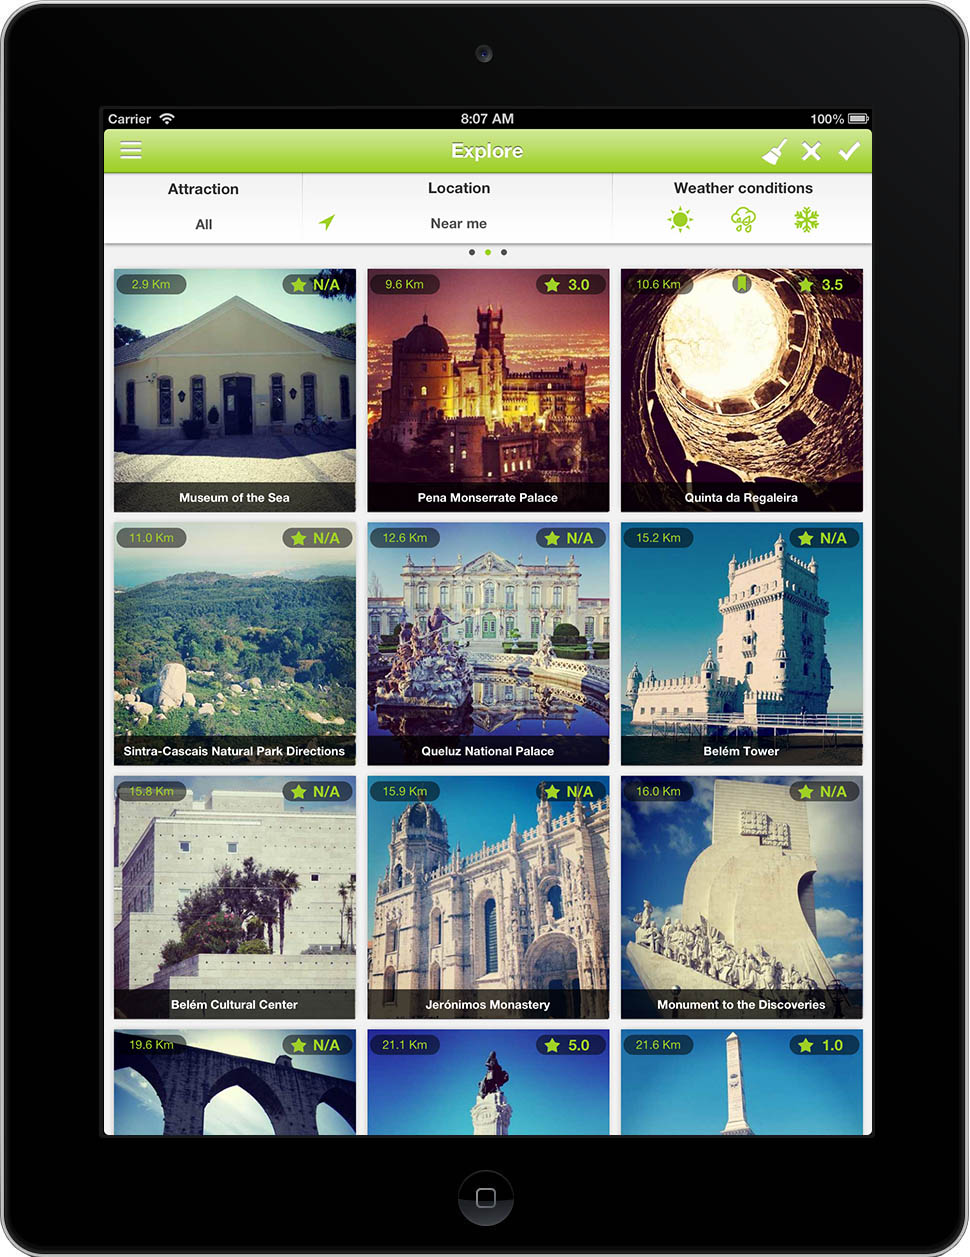
\includegraphics[height=8cm]{./images/screenshots/screenshot_ipad_app_1.jpg}
                \caption{Location search.}
                \label{fig:guidemeWebScreenshotsiPadFina1}
        \end{subfigure}
        \begin{subfigure}[b]{0.45\textwidth}
 				\centering
                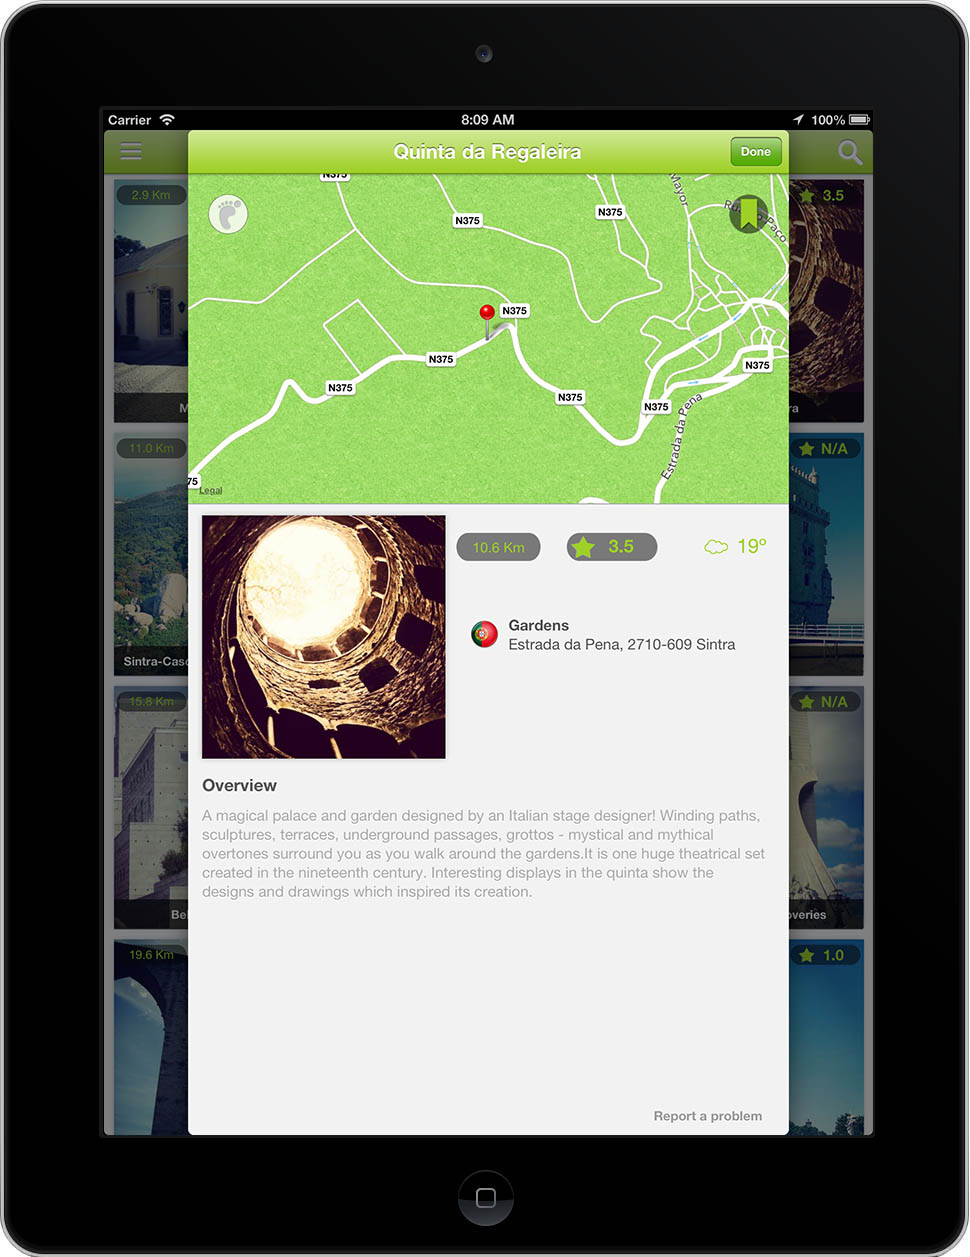
\includegraphics[height=8cm]{./images/screenshots/screenshot_ipad_app_2.jpg}
                \caption{Location details.}
                \label{fig:guidemeWebScreenshotsiPadFina2}
        \end{subfigure}
        \caption{Screenshots of the iPad application}
        \label{fig:guideMeWebScreenshotsiPadFull}
        \end{center}
\end{figure}\\
The full set of features for each version of the application is documented and located in the \emph{GuideMeMobileClient} repository.
%%%%%%%
%%%%%%%
\subsection{Internationalization}
\label{subsec:iosInternationalization}
The developed application provides translation strings for the English and Portuguese languages. If the user has configured any language other than English or Portuguese, the application assumes English by default. During the remote requests, the language identifier\footnote{The language identifier in the iOS application is defined in ISO 639-1 format. The same type of locale identifiers is supported by the REST API.} used for loading localized resources is passed to our REST API, ensuring that the information is retrieved using the same locale as the one configured by the device.

%%%%%%%
%%%%%%%
\section{Push Notifications}
\label{subsec:pushNotificationIntro}
We use the~\gls{apns} service to notify users about important events that occur regarding them. A use case of this concept, is when the user is followed by another, the push notification is sent detailing the occurred event as illustrated on Figure~\ref{fig:pushNotificationExamle}, otherwise this action could pass unnoticeable to the followed user.\\
\begin{figure}[h!]
 \centering
   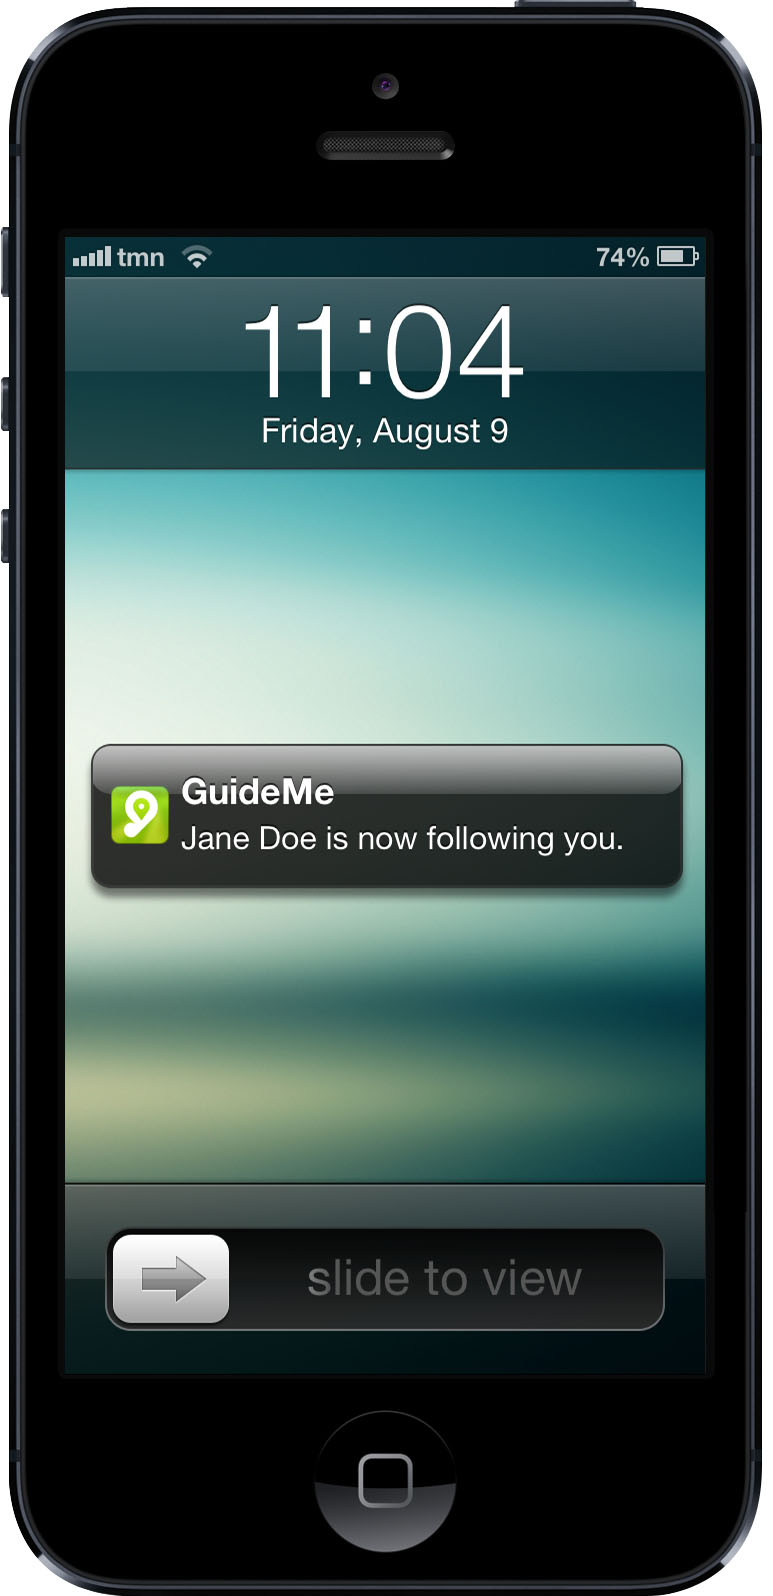
\includegraphics[height=6cm]{./images/screenshots/screenshot_push_notification_example.jpg}
   \caption{An example of the push notification sent by GuideMe service.}
   \label{fig:pushNotificationExamle}
\end{figure}\\
To implement this feature, we have used the Java-APNS~\cite{javaApns} implementation that already solves many of the difficulties, such as, communication with the APNS, establishing of a secure connection, among others. In order to make the provider communicate with the APNS and later the APNS with the device, it was required to correctly configure the certificate in Java-APNS framework and the Provisioning Profile~\cite{appleRemoteNotifProvisioning} during the deployment of the mobile applications\footnote{To develop and deploy the provider side of an application for push notifications, it is required  to obtain the SSL certificates from the appropriate Apple Developer Center~\cite{appleIosDeveCenter}.}. Each certificate is limited to a single application, identified by its bundle ID. It is also limited to one of two environments: development or production. These environments have their own assigned IP address and require their own certificates. It is also required to obtain provisioning profiles for each of these environments in order to receive the push notification when the application is deployed to the mobile device. The communication flow for sending the push notification, between the source and destination devices, is illustrated on Figure~\ref{fig:apnsUseCase}.\\
%%%%%%
\begin{figure}[h!]
 \centering
   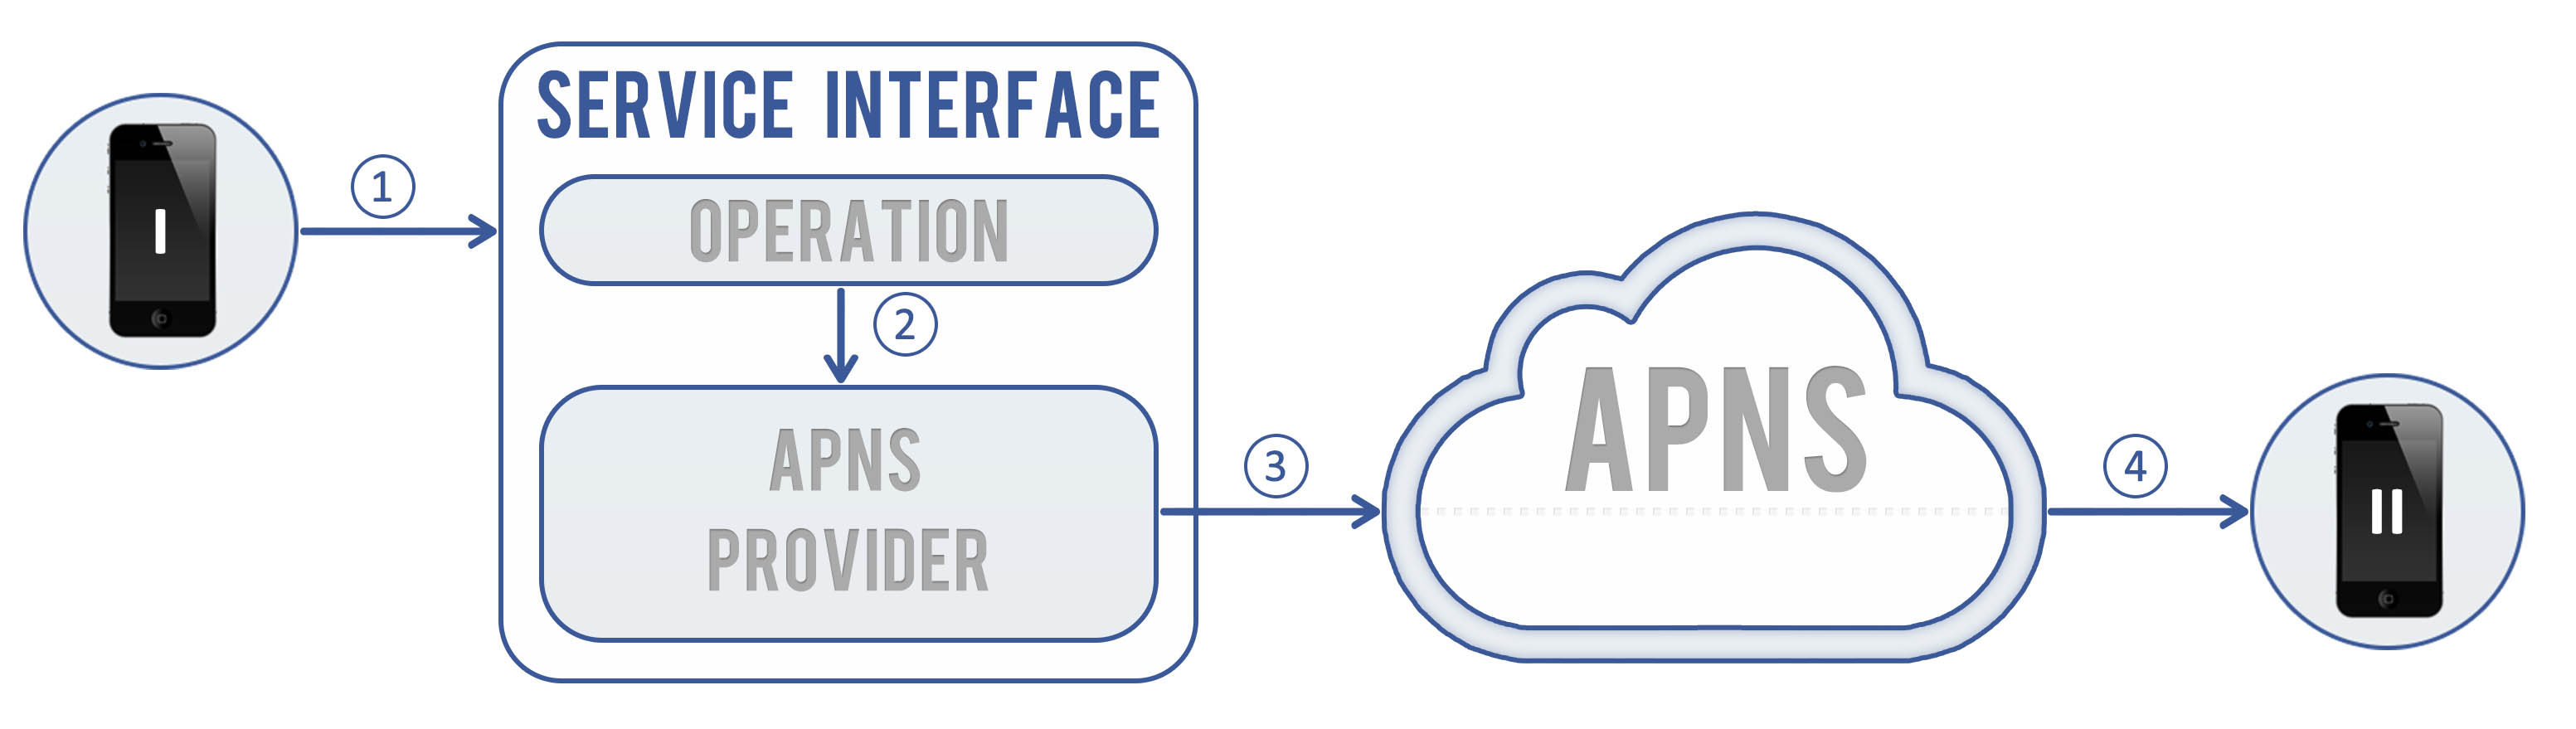
\includegraphics[height=2.8cm]{./images/diagrams/diagram_usecase_pushnotification.jpg}
   \caption{Delivery of the push notification to the destination device.}
   \label{fig:apnsUseCase}
\end{figure}\\
%%%%%%
The steps regarding the push notification delivery are as follows:
\begin{enumerate}
	\item The source device performs a remote request to execute an action (for example, follow some user).
	\item After a successfully performed operation, the routine from the APNS provider is invoked.
	\item A new notification is created and sent to the APNS server. 
	\item When possible, APNS delivers the notification to the destination device.
\end{enumerate}
%%%%%%
As it is stated by Apple, the provider is responsible for not propagating push notifications to devices that are not able to receive them. We have implemented a service, that is executed by Cron job every 10 minutes. This service connects to the APNS Feedback service and obtains the device tokens that have repeatedly reported failed-delivery attempts. Then, we update the database by deactivating the reported device tokens. This periodic service was implemented using the Java-APNS framework and uses the data access layers to update the status of the device token or report errors to the log database when it is necessary.
        
\section{Web Application}
\label{sec:mobileApp}
In this Section, we describe the development aspects of the Web application. We detail the features and functionalities offered by this application.
%%%%%%%%%%
\subsection{Implementation Details}
\label{subsec:webAppImplementation}
The Web application was developed using the same framework as the REST API. Play Framework offers powerful Scala\footnote{Scala is an object-functional programming and scripting language for general software applications, statically typed, designed to concisely express solutions in an elegant, type-safe and lightweight manner.} template engine which was inspired by ASP.NET Razor~\cite{aspNetRazor}. The template system was designed in a manner that facilitates the development of the web applications, where the \verb"'@'" character indicates the Scala statement and it does not require to explicitly close the code-block. An example of the template engine is shown in Code Listing~\ref{cod:playWebExample}.\\
\begin{lstlisting}[language=HTML,caption={An example of the Scala template.},label={cod:playWebExample}, frame=bt, belowskip=3em]
@(location: LocationModel)
@if(location == null){
   <h1>Location is invalid</h1>
}else{
   <h2>location.getTitle()</h2>
   <ul>
      @for(user <- location.visitedBy()) { <li>@user.name</li> }
   </ul>
}
\end{lstlisting} 
%%%%%%%
The Play application follows the~\gls{mvc} architectural pattern applied to the Web architecture. This pattern splits the application into separate layers: the Presentation layer and the Model layer. The Presentation layer is further split into a View and a Controller layer. The Model holds the domain-specific representation of the information on which the operation executes. The View renders the model into a form suitable for interaction, while the Controller responds to the~\gls{http} Requests and applies changes to the underlying model. The Views are designed using the Bootstrap~\cite{twitterBootstrap} which is designed for faster and easier Web development. It defines a set of generic components and layouts which are used across the application and removes the compatibility barrier between different browsers.
%%%%%%%%%%
%%%%%%%%%%
\subsection{Web Application Overview}
\label{subsec:webAppOveriew}
The Web application implements a subset of functionalities of the mobile application. It allows to users authenticate using their Facebook account, consult visited, wanted and recommended locations, and the detailed information of each location. They can visualize their profile page with the information regarding the current account. On the details page of the touristic point, users can consult the exact location through the Google Maps service.\\
\\
The Figure~\ref{fig:guideMeWebScreenshotsFull}~(\subref{fig:guidemeWebScreenshotsFina1}) illustrates the page with a set of visited locations. By selecting any of the listed locations, its details are shown in a similar way as one from Figure~\ref{fig:guideMeWebScreenshotsFull}~(\subref{fig:guidemeWebScreenshotsFina2}).
\begin{figure}
        \begin{subfigure}[b]{0.5\textwidth}
                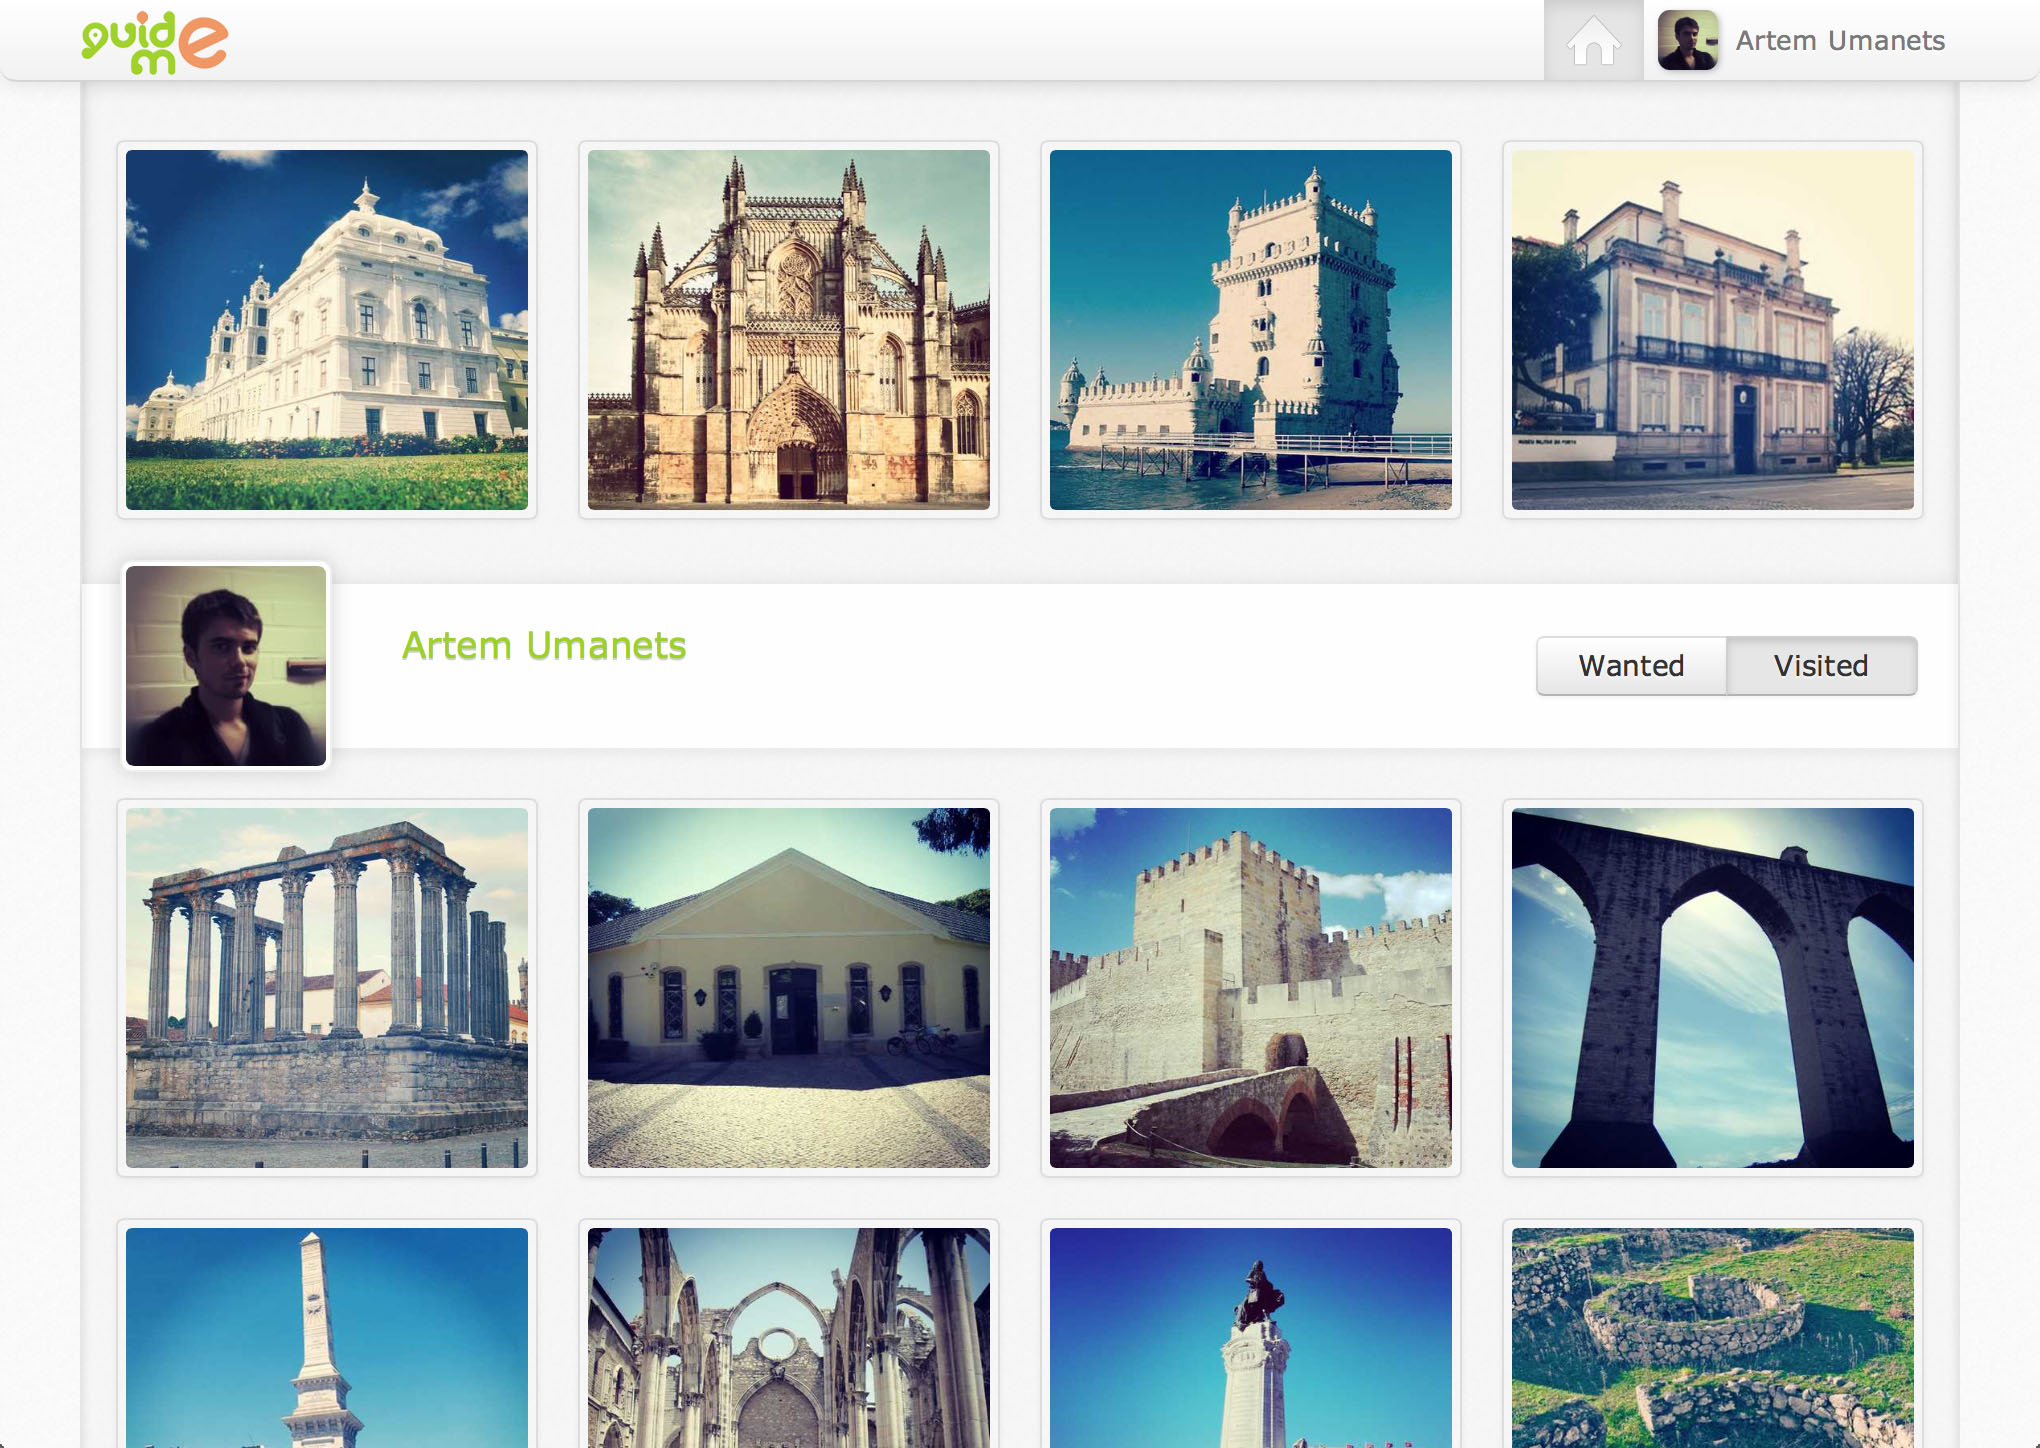
\includegraphics[height=5.2cm]{./images/screenshots/screenshot_web_app_1.jpg}
                \caption{Visited locations.}
                \label{fig:guidemeWebScreenshotsFina1}
        \end{subfigure}%
        \begin{subfigure}[b]{0.5\textwidth}
                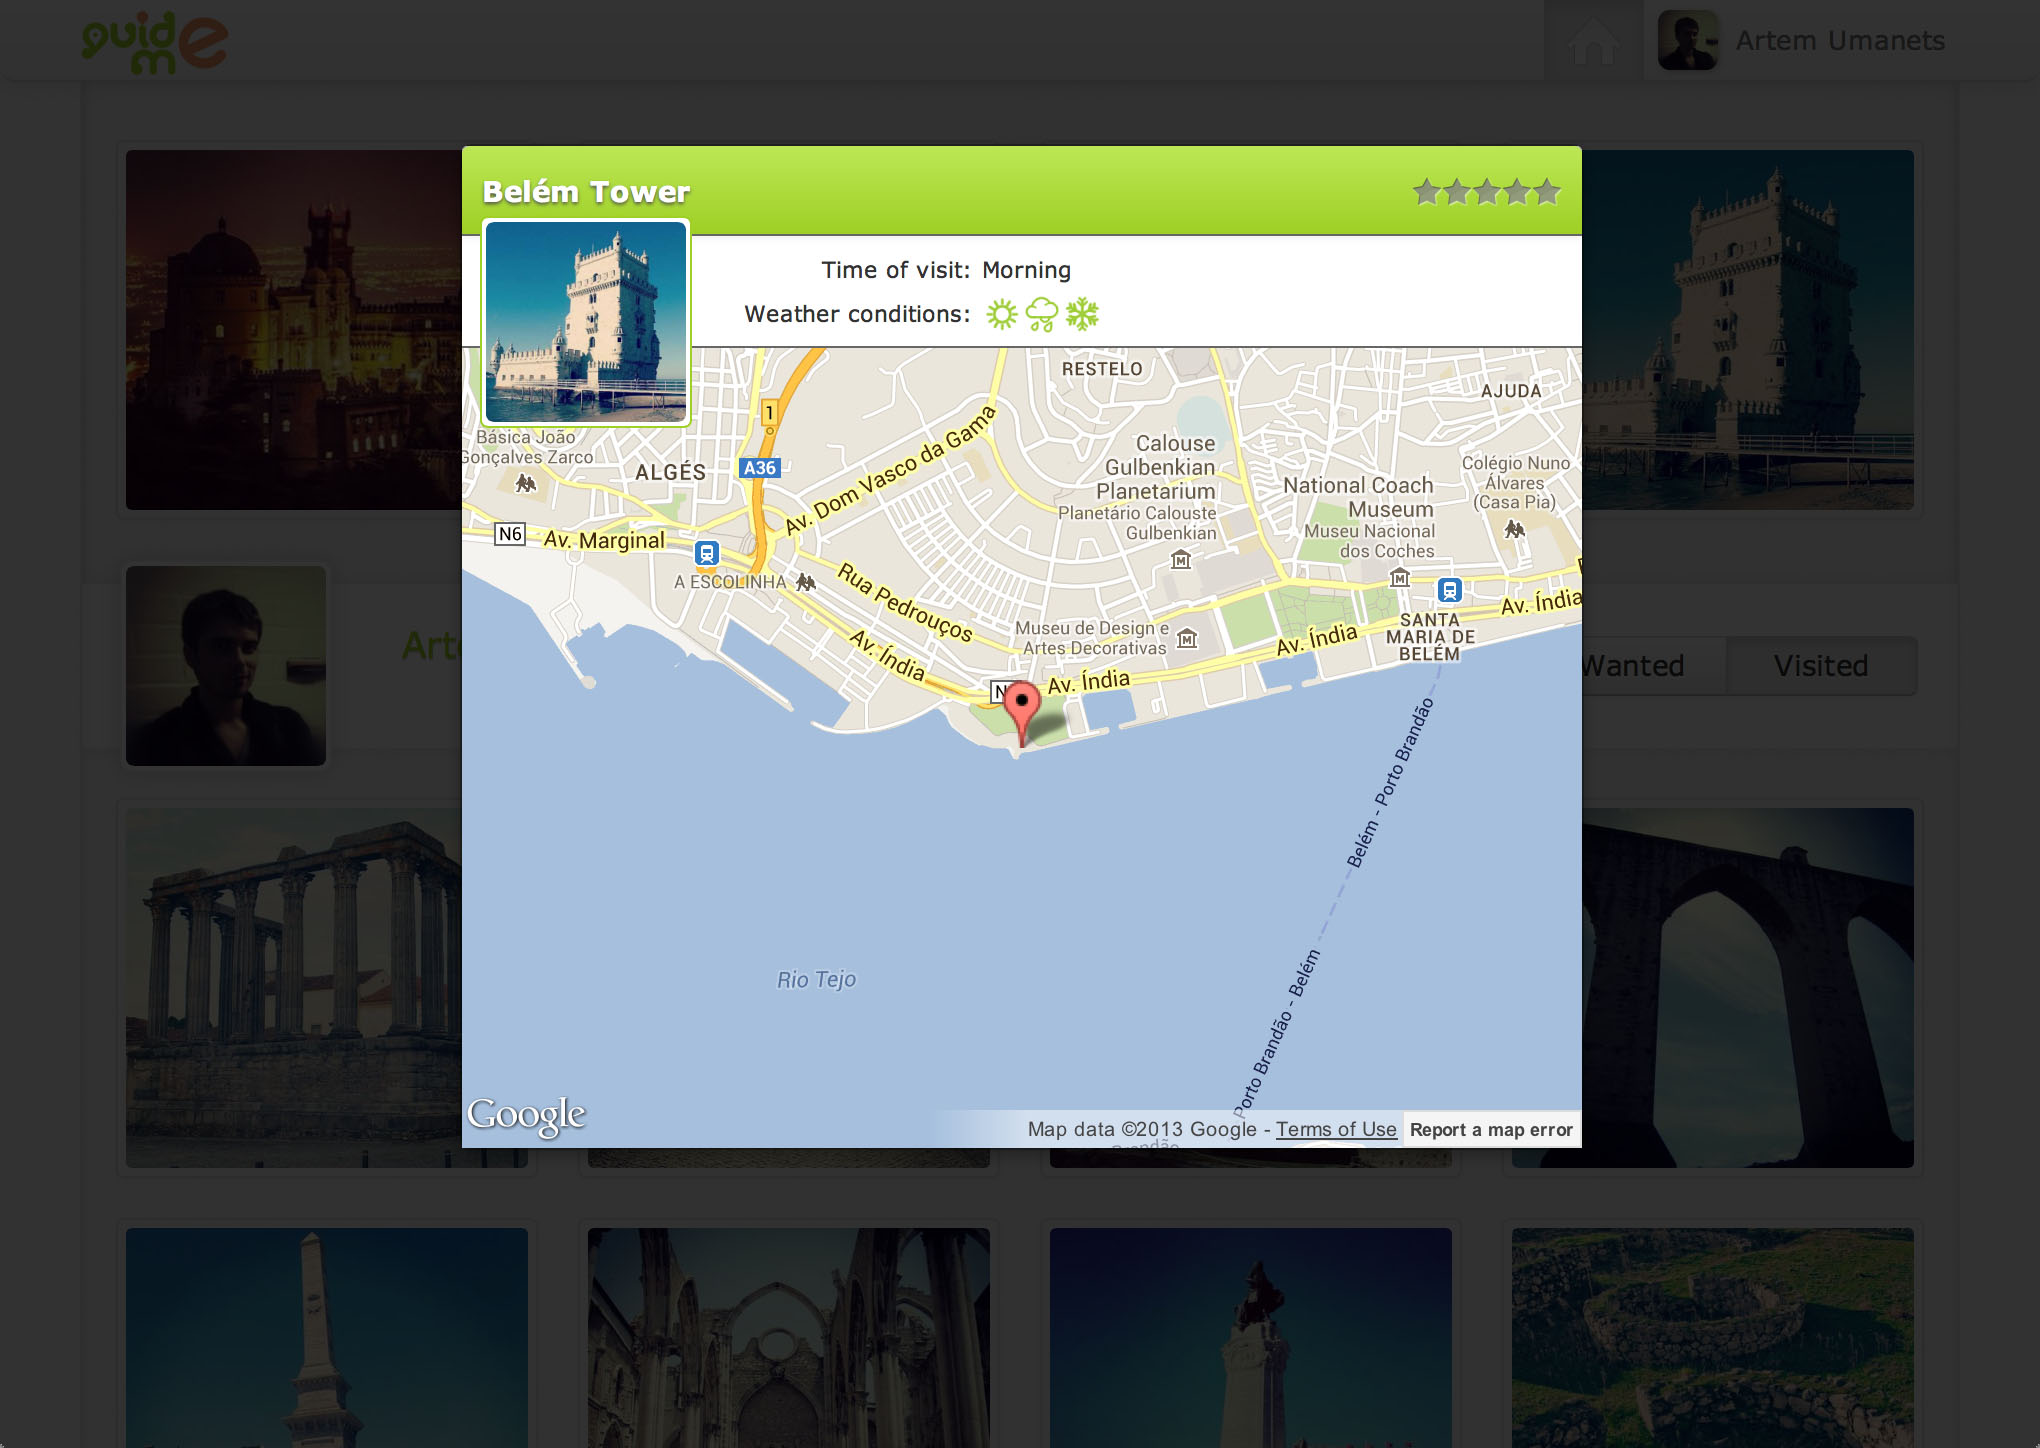
\includegraphics[height=5.2cm]{./images/screenshots/screenshot_web_app_2.jpg}
                \caption{Location details.}
                \label{fig:guidemeWebScreenshotsFina2}
        \end{subfigure}
        \caption{Screenshots of the Web application}
        \label{fig:guideMeWebScreenshotsFull}
\end{figure}
%%%%%%%%%%
%%%%%%%%%%
\subsection{Internationalization Support}
\label{subsec:webAppInternationaization}
The Web application supports localized content using the same mechanism as the \gls{rest}~\gls{api}. The HTTP cookie~\cite{httpCookie} with the language identifier is populated on the first request, and by default it refers to the English language. The action that changes the language overrides the language identifier with a new value which can be changed from either the login or profile page.\\
\\
Some Web operations are implemented in asynchronous mode using the \gls{js} and \gls{ajax} technologies in order to make the user's interaction more intuitive. We have used jQuery~\cite{jquery} library to make the development of the \gls{js} code easier and more readable. The Scala template engine is not able to parse the external \gls{js} files, so a problem with localized messages appeared when it became necessary to show messages to user through \gls{js}. The solution that was found consisted in using the extension for i18n properties for the jQuery library, consist in performing the \gls{ajax} request to the implemented endpoint \verb"/i18n", which returns the content of the appropriate messages file from the \verb"/conf" directory. Then the localized messages can be accessed as follows: \verb"$.i18n.prop(""\verb"MessageKey""\verb")".
%%%%%%%
%%%%%%%
\subsection{REST API Documentation}
\label{subsec:restAPIDcos}
Users with the administrative role can consult the documentation of the \gls{rest}~\gls{api} on their profile page. Each endpoint is described as a separate text file located in the \verb"public/api" directory. The template for the documentation file is shown in Code Listing~\ref{cod:docFileStrcuture}:\\
\begin{lstlisting}[language=Java,caption={Organization of the documentation information.},label={cod:docFileStrcuture}, frame=bt,belowskip=3em]
@->Title:<Title>
@->Description:<Endpoint Description>
@->Method:<HTTP Method>
@->Url:<Endpoint URL>
@->AuthenticationRequired:<Indicates when authentication is required>
@->Permission:<User Permissions>
@->RequiredParameters:
param1[Type] - Description of parameter1
...
@->OptionalParameters:
param2[Type] - Description of parameter2
...
@->CallExampleUrl:<Example of the invocation URL>
@->OutputExample:<Example of the response, usually in JSON format>
\end{lstlisting} 
Each property is separated by \verb"@->" and the first \verb':' separates the property name from its content. The endpoints are obtained by listing all the files from the \verb"public/api" directory. Each of them is mapped into a model that is more easily integrated in the Scala template. An example illustrating the organization of the endpoint documentation is shown in Figure~\ref{fig:exDocEntry}.\\
\begin{figure}[h!]
 \centering
   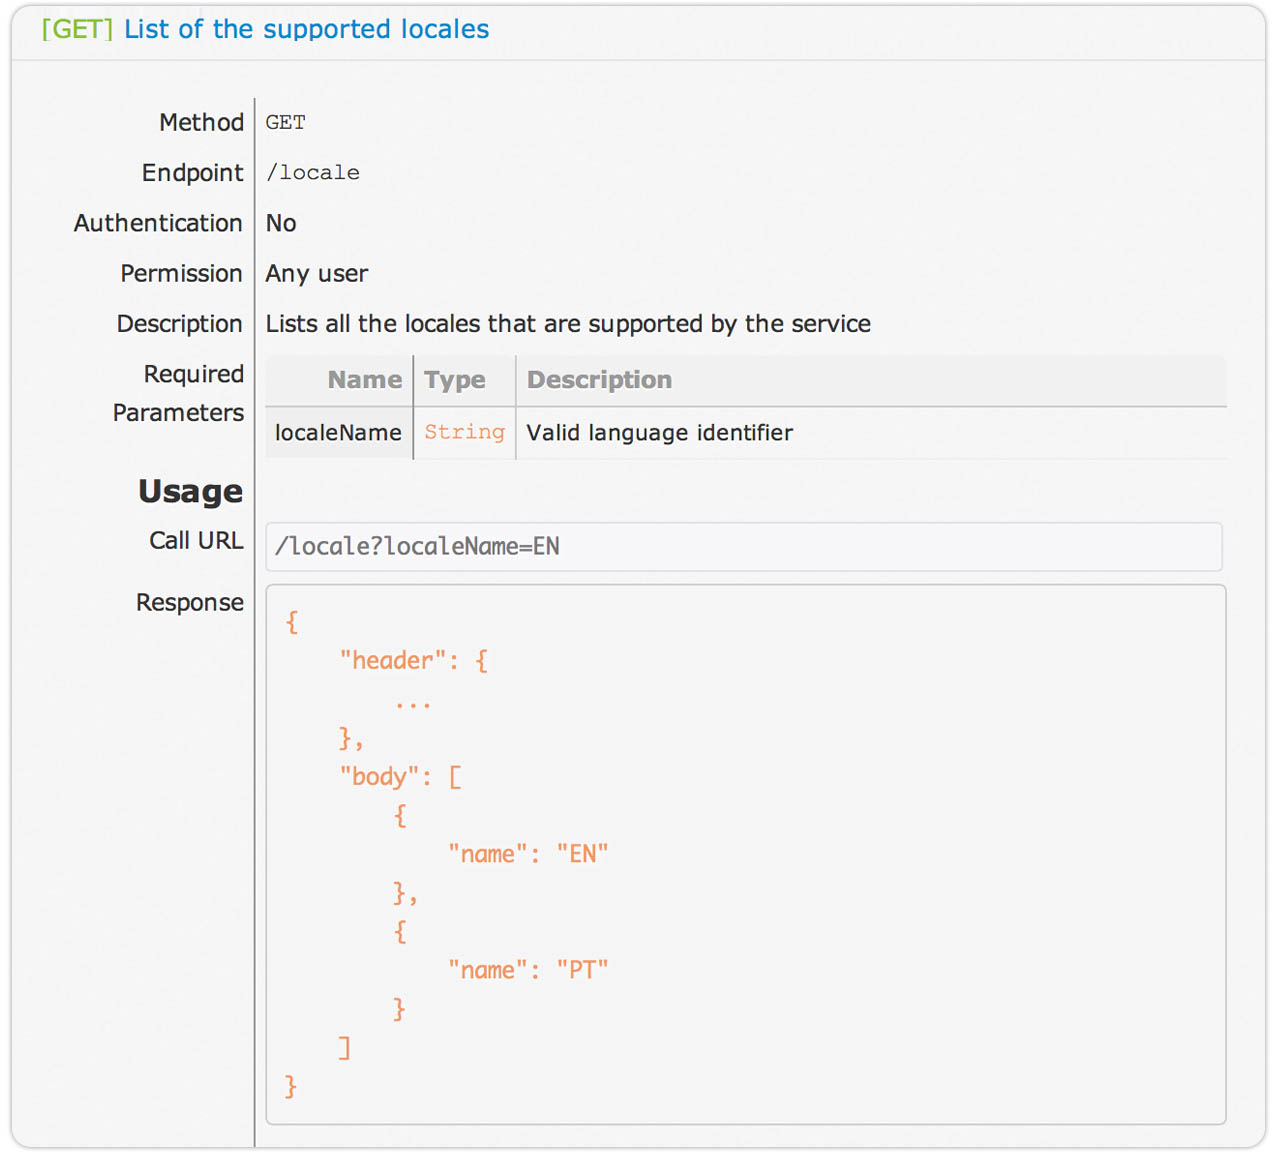
\includegraphics[width=9cm]{./images/examples/example_webapp_documentation.jpg}
   \caption{An example of the documentation entry.}
   \label{fig:exDocEntry}
\end{figure}
\\
The approach for reading and parsing the documentation data is not very efficient. The usage of the database would be more appropriate but we did not want to introduce more databases and complexity to the current project. Improving this part of the project is one of the goals in the future.
%%%%%%%%%%
%%%%%%%%%%
\section{Additional Developments}
\label{sec:additionalImplementation}
In this Section, we describe other developments that were made for this project.
%%%%%
\subsection{Software Testing}
\label{subsec:softwareTesting}
Unitary test methodology is used to check the quality of the code and to facilitate the detection of bugs that may be discovered in the future. Currently, there are around 120 unit test for the \gls{rest} \gls{api} service and 190 unitary test for the Service and Log \gls{dal}. All unitary tests share the same pre-populated database and perform different kinds of operations and queries to ensure that the tested operations perform correct actions.\\
\\
In order to analyse the code coverage, we have used the EclEmma~\cite{codeCoveragEclEmma} plugin for Eclipse IDE. This analysis helped us to improve coverage of the implemented unit tests, lowering the chance of bugs. The implemented unit tests are covering around $90\%$ of the code related to the Service DAL and around $75\%$ of the Log DAL. The uncovered code is mainly related to the entities generated by the Hibernate framework.\\
\\
The iOS application implements 35 unit tests which aim is to perform the remote requests to the~\gls{rest} API. These tests help to detect any unpredictable changes that may emerge in the future.
%%%%%
\subsection{Multi Environment Support}
\label{subsec:multiEnvironmentSupport}
The DAL and~\gls{rest} API components were carefully designed in order to support multiple environments by mean of configuration. At the DAL layer, it is possible to specify different configuration files for testing and production purposes. The same applies to the~\gls{rest} API, which allows to adjust the configurations that vary between test and production environments.

\subsection{REST API Incoherence}
\label{subsec:restAPIIncoherence}
The developed \gls{rest} API invalidates some concepts of the \gls{rest} architecture due to external causes. Usually, the \verb"DELETE HTTP" method is used for resource removal and \verb"UPDATE HTTP" method updates the resource. Some firewalls may block these HTTP verbs, therefore the API was developed in order to use the POST method for creating, updating and removing the resource and GET to consult its information. The type of the operation is indicated as part of the URL request (e.g. the operation to remove the user is implemented as follows: POST \url{http://host/user/delete?id=5} instead of DELETE \url{http://host/user/5}).
%\chapter{Experimental Results}
\label{sec:ExpResults}

In this section we will present the results obtained while running all the heuristics explained in the previous chapters. We will also compare the obtained results with the top 5 winners of the ITC2007.\\
\\
The results obtained using the approach explained in the previous chapters were not as we expected. Some of the results obtained could be as good as it can match the top 5 winners, and some were so far away from these. Each set score is the result of the average of 10 runs that were done on that same set. The tests were made on all 12 sets, including the hidden ones.\\
\\
The parameters used to run the Simulated Annealing and the Hill Climbing were:\\
\\
TMax $\rightarrow$ 0.01\\
TMin $\rightarrow$ $1e^{-18}$\\
reps $\rightarrow$ 5\\
rate $\rightarrow$ 0.001\\

With these parameters used on all the sets, we obtained the results presented on the Table \ref{tab:ITC2007ResultsComparison}. As can be seen, the results for the sets 1, 2, 6, 7, 8 and 9 can match the 5 winners' results, but the sets 3, 10 and 11 were way too far away from the results of the top 5 (the ones that could get a feasible solution). We believe this can be fixed by tweaking the parameters and give individual parameters to each set to try and obtain better results.\\
\\
\begin{table*}
\centering

\sisetup{table-alignment=center,detect-weight=true,detect-inline-weight=math}
\begin{tabular}{%
	S[table-figures-integer=2]%
	S[table-format=5.1]%
	S[table-format=5.1]%
	S[table-format=5.1]%    
	S[table-format=5.1]%
	S[table-format=5.1]%
	S[table-format=5.1]%
    }

\toprule

\multicolumn{1}{l}{Instance} & \multicolumn{1}{l}{M\"{u}ller} &	\multicolumn{1}{l}{Gogos et} & \multicolumn{1}{l}{Atsuta et} & \multicolumn{1}{l}{De Smet} & \multicolumn{1}{l}{Pillay} & \multicolumn{1}{l}{My Approach}\\
		& \multicolumn{1}{l}{2008 \cite{Mueller2009}} & \multicolumn{1}{l}{al. 2008~\cite{Gogos2012}} & \multicolumn{1}{l}{al. 2008~\cite{Atsuta2007}} & \multicolumn{1}{l}{2008~\cite{Smet2007}} & \multicolumn{1}{l}{2008~\cite{Pillay2007}} & \multicolumn{1}{l}{2015} \\

\midrule

1   &   \boldentry{5.1}{4370}  & 5905      & 8006           & 6670       & 12035 & 6934\\
2   &   \boldentry{5.1}{400}   & 1008      & 3470           &  623       & 3074 & 821 \\
3   &   \boldentry{5.1}{10049} & 13862     & 18622          & \text{--}  & 15917 & 24627 \\
4   &   \boldentry{5.1}{18141} & 18674     & 22559          & \text{--}  & 23582 & \text{--} \\
5   &   \boldentry{5.1}{2988}  & 4139      & 4714           & 3847       & 6860 & 7729\\
6   &   \boldentry{5.1}{26950} & 27640     & 29155          & 27815      & 32250 & 30195 \\
7   &   \boldentry{5.1}{4213}  & 6683      & 10473          & 5420       & 17666 & 8089 \\
8   &   \boldentry{5.1}{7861}  & 10521     & 14317          & \text{--}  & 16184 & 11067 \\
9   &   \boldentry{5.1}{1047}  & 1159      & 1737           & 1288       & 2055 & 1448 \\
10  &   16682                  & \text{--} & 15085          & \boldentry{5.1}{14778}      & 17724  & 35698\\
11  &   \boldentry{5.1}{34129} & 43888     & \text{--}      & \text{--}  & 40535 & 72751 \\
12  &   5535            & \text{--} & \boldentry{5.1}{5264} & \text{--}  & 6310 & 8049 \\

\bottomrule

\end{tabular}
\caption{ITC 2007 results comparison to this project's approach. The best solutions are indicated in bold. ''--'' indicates that the corresponding instance is not tested or a feasible solution cannot be obtained.}
\label{tab:ITC2007ResultsComparison}
\end{table*}
%\chapter{Conclusions}
\label{conclusions}



%\appendix
\chapter{Appendix}
\label{attachments}
In this Chapter, we have included some implementation which is referenced along with the current report.

\section{Service Database - Entity Relationship Model}
\label{sec:ServiceDatabase}
Figure~\ref{fig:serviceDatabaseER} shows the ER model which describes the Service Database.

\begin{figure}[h!]
 \centering
   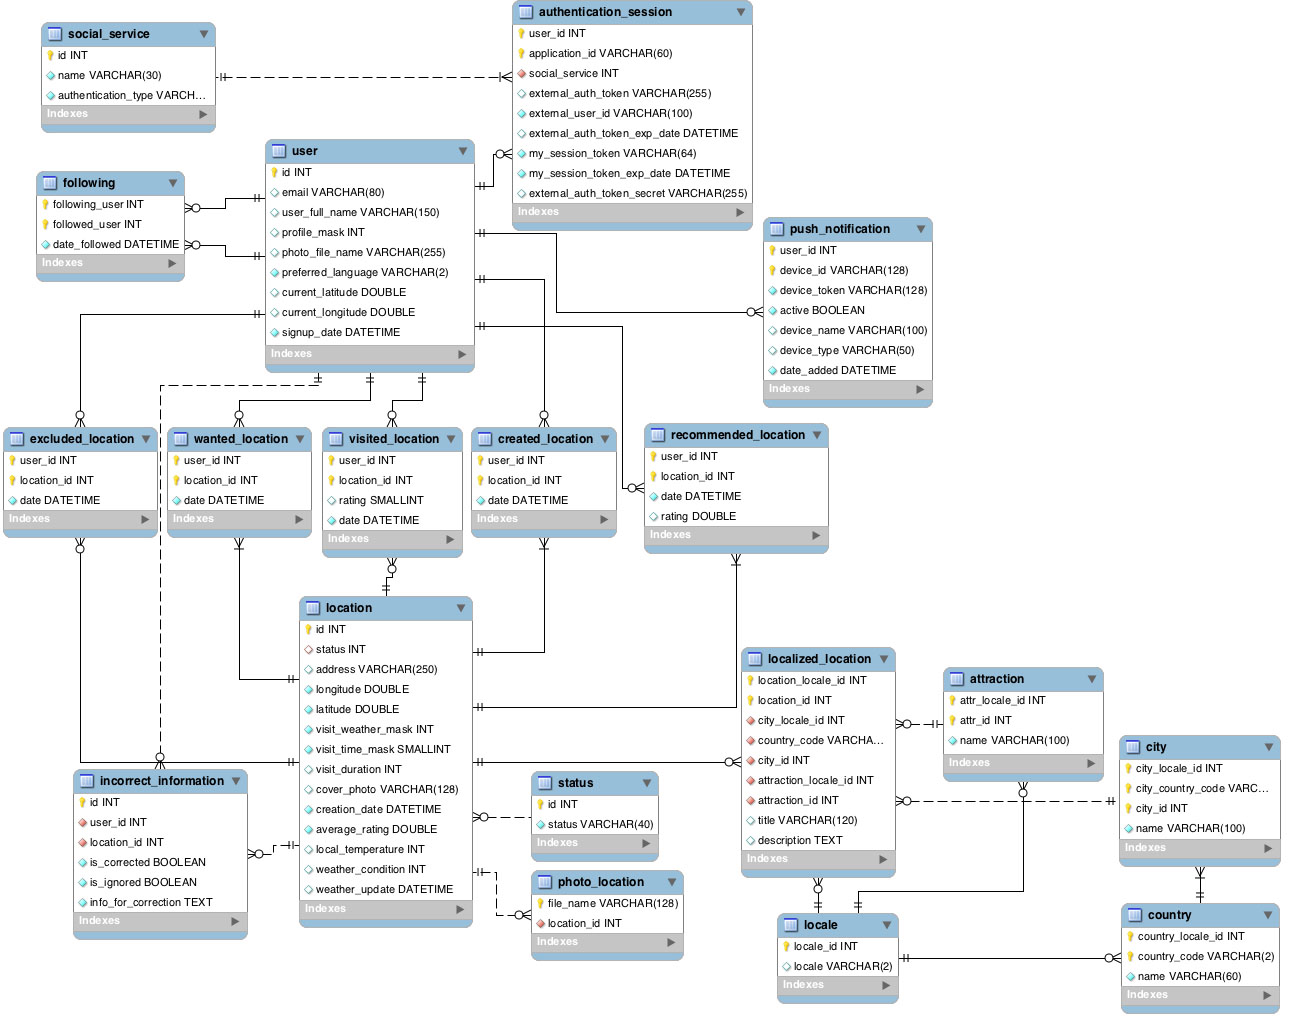
\includegraphics[width=12.8cm]{./images/umls/uml_dbmodel_service.jpg}
   \caption{Service Database ER model.}
   \label{fig:serviceDatabaseER}
\end{figure}
\newpage

\section{Log Database - Entity Relationship Model}
\label{sec:AttachmentsLogDatabase}
Figure~\ref{fig:logDatabaseER} shows the ER Model which describes the Log Database. It allows tracking of the different events that may occur (errors, warnings, among others) for different service components.

\begin{figure}[h!]
 \centering
   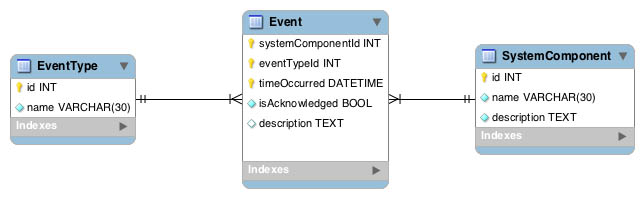
\includegraphics[width=12cm]{./images/umls/uml_dbmodel_log.jpg}
   \caption{Log Database ER model.}
   \label{fig:logDatabaseER}
\end{figure}
\newpage

\section{Usability Evaluation Survey}
\label{sec:survey}
This Section contains a questionnaire that have been used during the usability evaluation process.
\begin{figure}[h!]
 \centering
   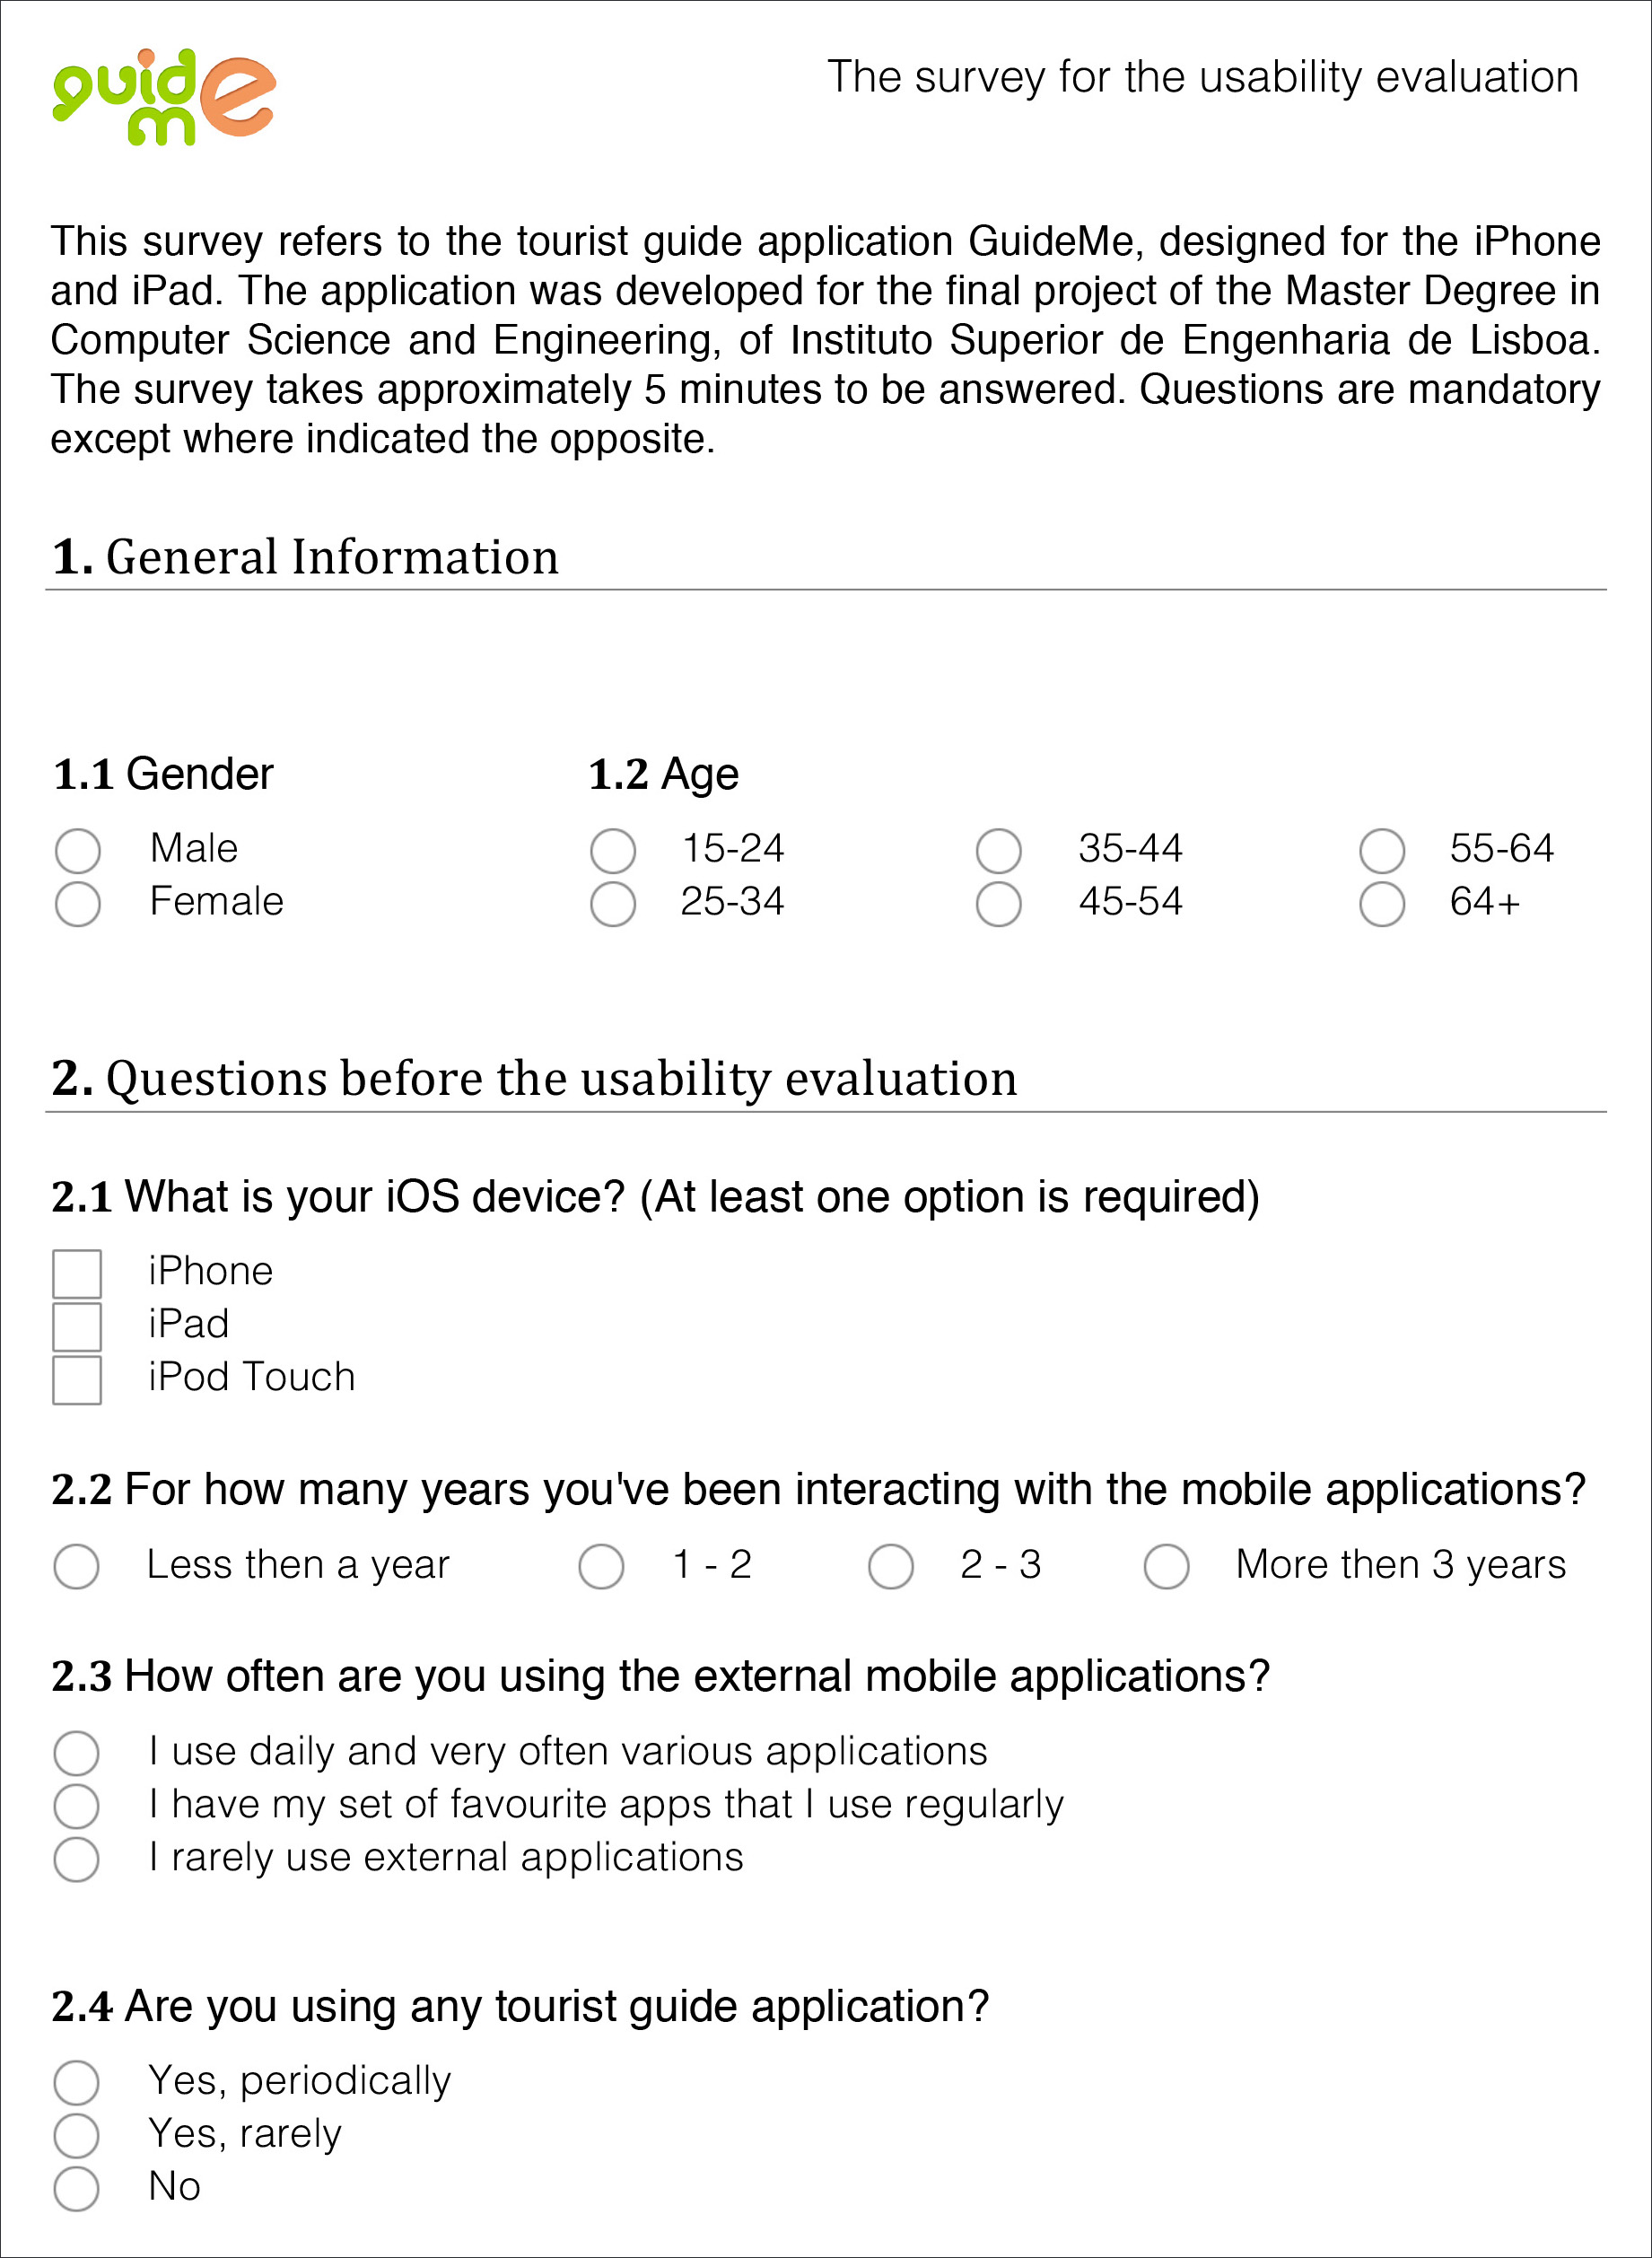
\includegraphics[width=12.5cm]{./images/survey/survey_page_1.jpg}
   \caption{Questionnaire - Page 1 of 3}
   \label{fig:surveyPage1}
\end{figure}
\newpage

\begin{figure}[h!]
 \centering
   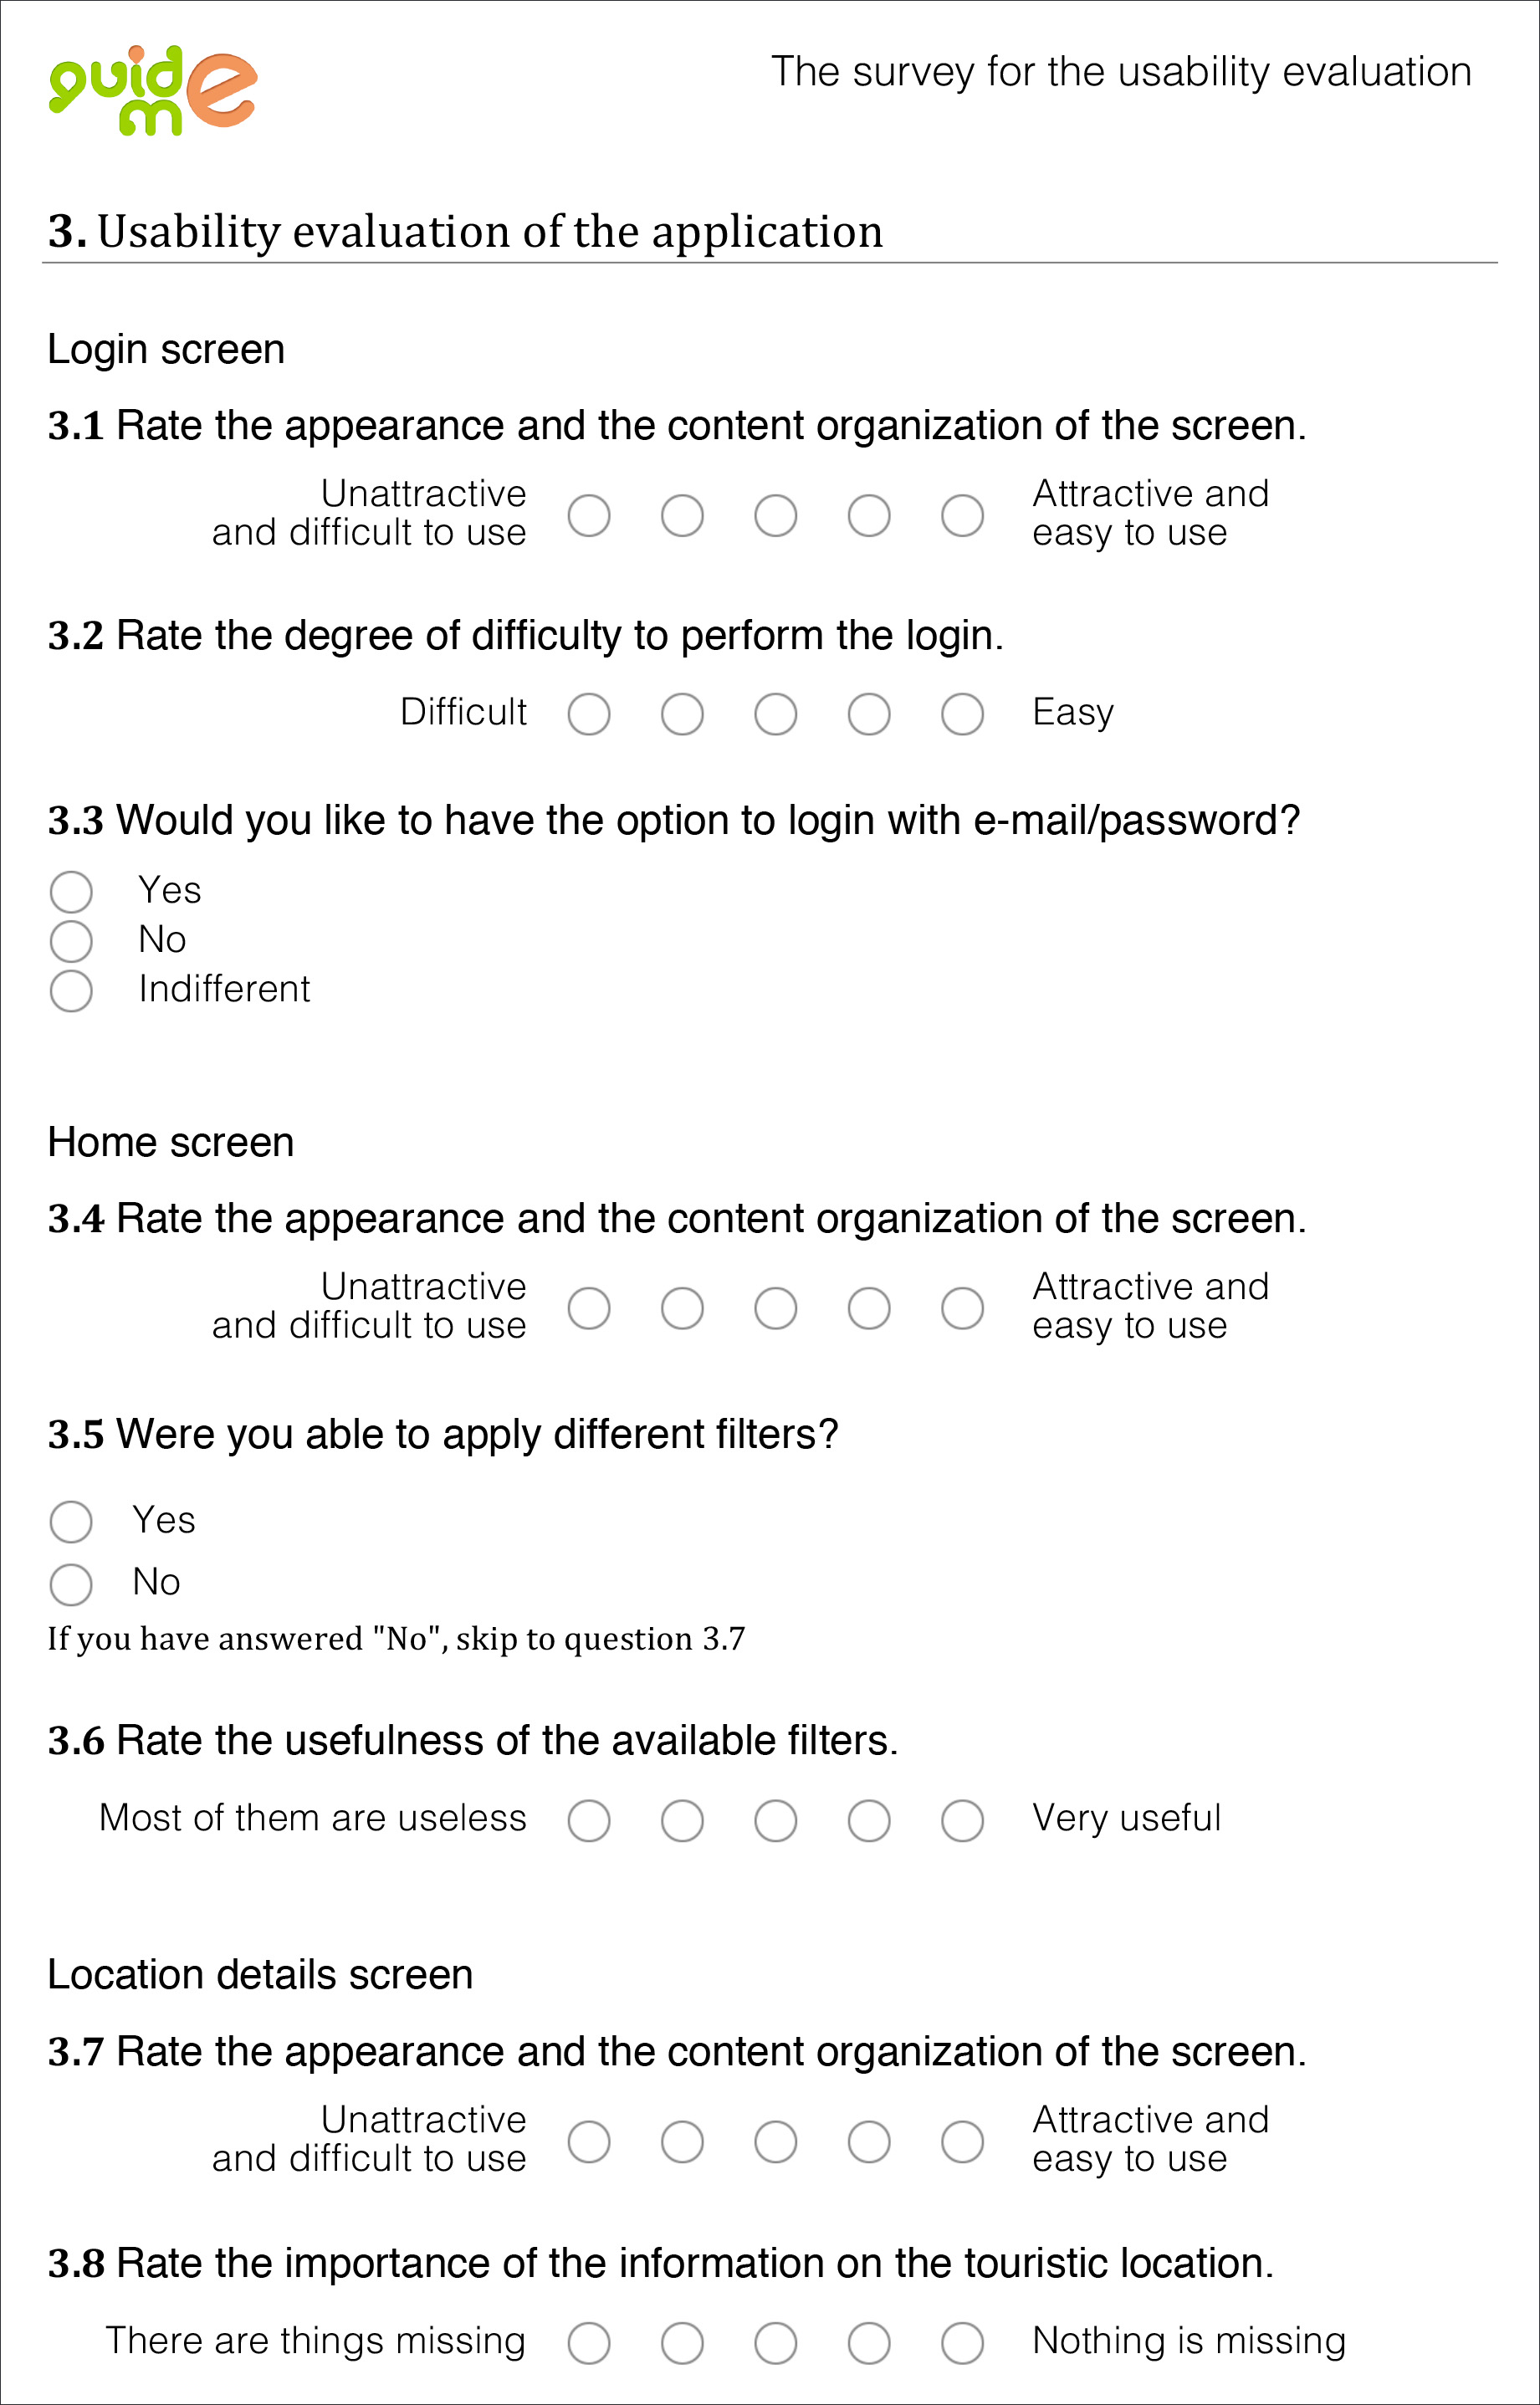
\includegraphics[width=12.5cm]{./images/survey/survey_page_2.jpg}
   \caption{Questionnaire - Page 2 of 3}
   \label{fig:surveyPage1}
\end{figure}
\newpage

\begin{figure}[h!]
 \centering
   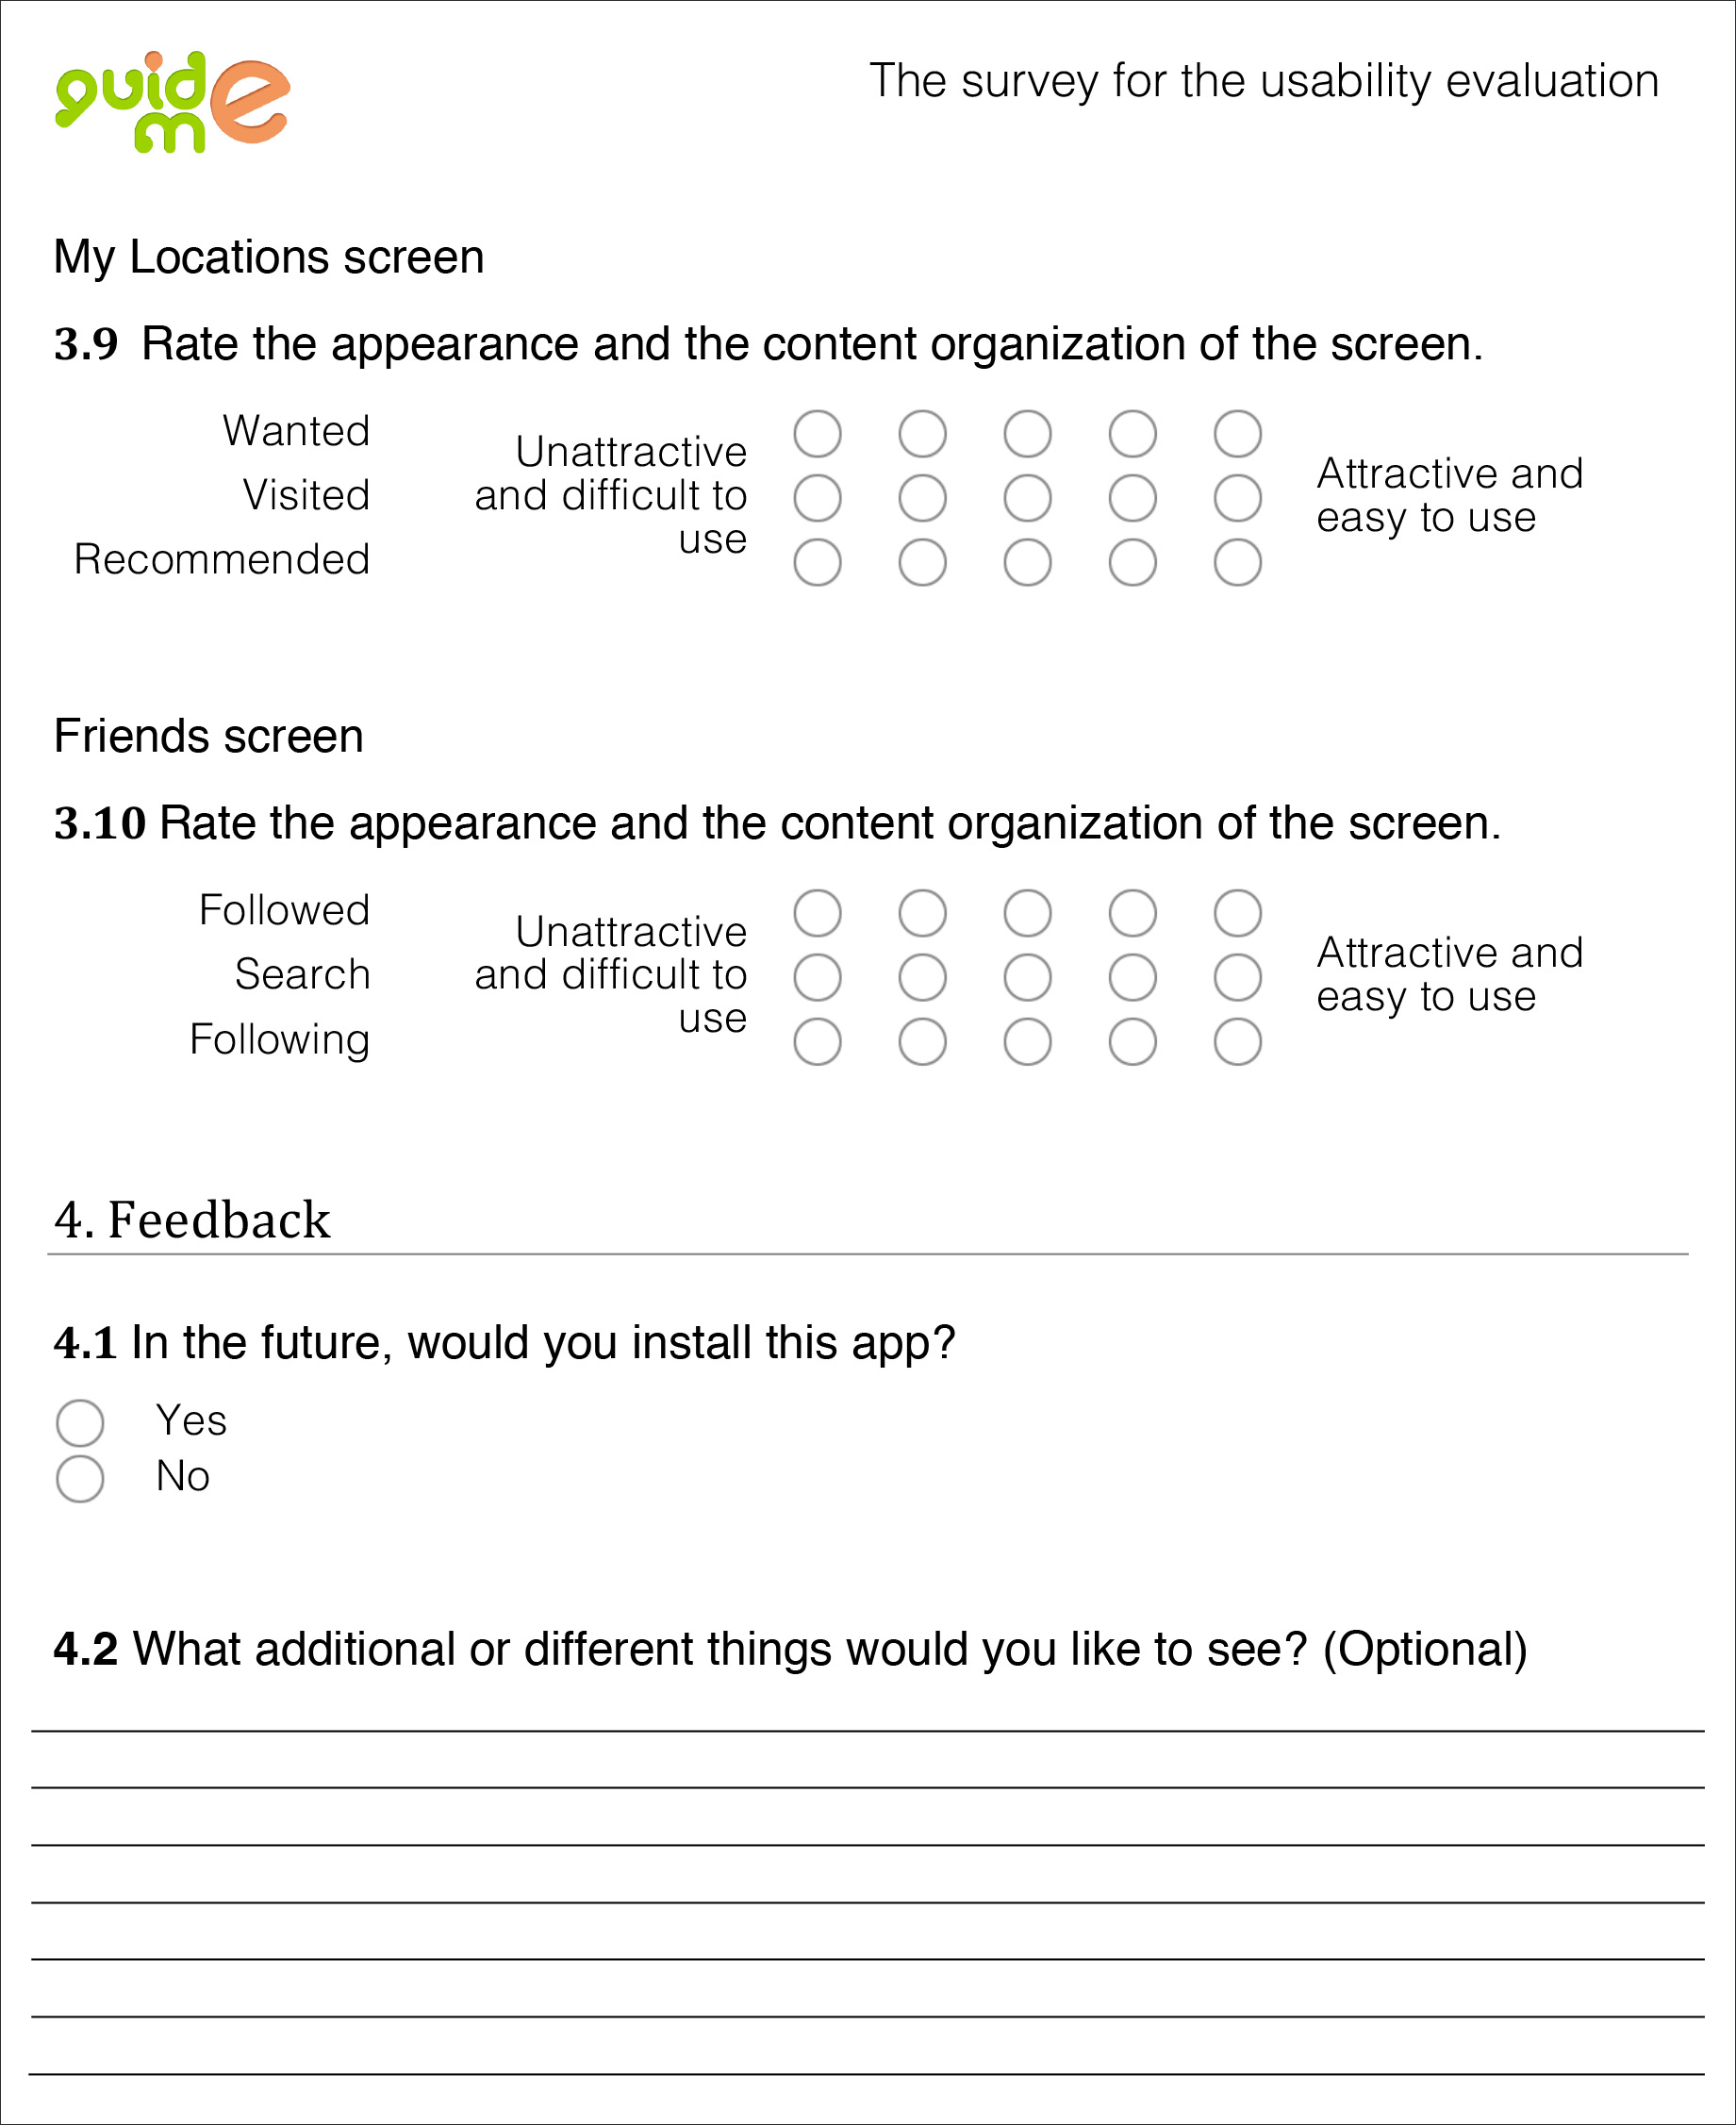
\includegraphics[width=12.5cm]{./images/survey/survey_page_3.jpg}
   \caption{Questionnaire - Page 3 of 3}
   \label{fig:surveyPage1}
\end{figure}

\backmatter					%%%%%%%%%%%%%%%%%%%%%%%%%%%%%%%%%%%%%%%%%%%%%%%%%%%
% BibTeX users please use
% \bibliographystyle{}
% \bibliography{}
%

\bibliographystyle{plain}
\bibliography{000-main}

\end{document}

